\documentclass[twoside]{book}

% Packages required by doxygen
\usepackage{fixltx2e}
\usepackage{calc}
\usepackage{doxygen}
\usepackage[export]{adjustbox} % also loads graphicx
\usepackage{graphicx}
\usepackage[utf8]{inputenc}
\usepackage{makeidx}
\usepackage{multicol}
\usepackage{multirow}
\PassOptionsToPackage{warn}{textcomp}
\usepackage{textcomp}
\usepackage[nointegrals]{wasysym}
\usepackage[table]{xcolor}

% Font selection
\usepackage[T1]{fontenc}
\usepackage[scaled=.90]{helvet}
\usepackage{courier}
\usepackage{amssymb}
\usepackage{sectsty}
\renewcommand{\familydefault}{\sfdefault}
\allsectionsfont{%
  \fontseries{bc}\selectfont%
  \color{darkgray}%
}
\renewcommand{\DoxyLabelFont}{%
  \fontseries{bc}\selectfont%
  \color{darkgray}%
}
\newcommand{\+}{\discretionary{\mbox{\scriptsize$\hookleftarrow$}}{}{}}

% Page & text layout
\usepackage{geometry}
\geometry{%
  a4paper,%
  top=2.5cm,%
  bottom=2.5cm,%
  left=2.5cm,%
  right=2.5cm%
}
\tolerance=750
\hfuzz=15pt
\hbadness=750
\setlength{\emergencystretch}{15pt}
\setlength{\parindent}{0cm}
\setlength{\parskip}{3ex plus 2ex minus 2ex}
\makeatletter
\renewcommand{\paragraph}{%
  \@startsection{paragraph}{4}{0ex}{-1.0ex}{1.0ex}{%
    \normalfont\normalsize\bfseries\SS@parafont%
  }%
}
\renewcommand{\subparagraph}{%
  \@startsection{subparagraph}{5}{0ex}{-1.0ex}{1.0ex}{%
    \normalfont\normalsize\bfseries\SS@subparafont%
  }%
}
\makeatother

% Headers & footers
\usepackage{fancyhdr}
\pagestyle{fancyplain}
\fancyhead[LE]{\fancyplain{}{\bfseries\thepage}}
\fancyhead[CE]{\fancyplain{}{}}
\fancyhead[RE]{\fancyplain{}{\bfseries\leftmark}}
\fancyhead[LO]{\fancyplain{}{\bfseries\rightmark}}
\fancyhead[CO]{\fancyplain{}{}}
\fancyhead[RO]{\fancyplain{}{\bfseries\thepage}}
\fancyfoot[LE]{\fancyplain{}{}}
\fancyfoot[CE]{\fancyplain{}{}}
\fancyfoot[RE]{\fancyplain{}{\bfseries\scriptsize Generated by Doxygen }}
\fancyfoot[LO]{\fancyplain{}{\bfseries\scriptsize Generated by Doxygen }}
\fancyfoot[CO]{\fancyplain{}{}}
\fancyfoot[RO]{\fancyplain{}{}}
\renewcommand{\footrulewidth}{0.4pt}
\renewcommand{\chaptermark}[1]{%
  \markboth{#1}{}%
}
\renewcommand{\sectionmark}[1]{%
  \markright{\thesection\ #1}%
}

% Indices & bibliography
\usepackage{natbib}
\usepackage[titles]{tocloft}
\setcounter{tocdepth}{3}
\setcounter{secnumdepth}{5}
\makeindex

% Hyperlinks (required, but should be loaded last)
\usepackage{ifpdf}
\ifpdf
  \usepackage[pdftex,pagebackref=true]{hyperref}
\else
  \usepackage[ps2pdf,pagebackref=true]{hyperref}
\fi
\hypersetup{%
  colorlinks=true,%
  linkcolor=blue,%
  citecolor=blue,%
  unicode%
}

% Custom commands
\newcommand{\clearemptydoublepage}{%
  \newpage{\pagestyle{empty}\cleardoublepage}%
}

\usepackage{caption}
\captionsetup{labelsep=space,justification=centering,font={bf},singlelinecheck=off,skip=4pt,position=top}

%===== C O N T E N T S =====

\begin{document}

% Titlepage & ToC
\hypersetup{pageanchor=false,
             bookmarksnumbered=true,
             pdfencoding=unicode
            }
\pagenumbering{roman}
\begin{titlepage}
\vspace*{7cm}
\begin{center}%
{\Large dokidoki \\[1ex]\large 0.\+1.\+0 }\\
\vspace*{1cm}
{\large Generated by Doxygen 1.8.11}\\
\end{center}
\end{titlepage}
\clearemptydoublepage
\tableofcontents
\clearemptydoublepage
\pagenumbering{arabic}
\hypersetup{pageanchor=true}

%--- Begin generated contents ---
\chapter{Namespace Index}
\section{Packages}
Here are the packages with brief descriptions (if available)\+:\begin{DoxyCompactList}
\item\contentsline{section}{\hyperlink{namespacedoki_battle}{doki\+Battle} }{\pageref{namespacedoki_battle}}{}
\item\contentsline{section}{\hyperlink{namespacedoki_script_compiler}{doki\+Script\+Compiler} }{\pageref{namespacedoki_script_compiler}}{}
\item\contentsline{section}{\hyperlink{namespacedoki_script_setting}{doki\+Script\+Setting} }{\pageref{namespacedoki_script_setting}}{}
\item\contentsline{section}{\hyperlink{namespacedoki_unity}{doki\+Unity} }{\pageref{namespacedoki_unity}}{}
\end{DoxyCompactList}

\chapter{Hierarchical Index}
\section{Class Hierarchy}
This inheritance list is sorted roughly, but not completely, alphabetically\+:\begin{DoxyCompactList}
\item \contentsline{section}{doki\+Script\+Setting.\+Action}{\pageref{classdoki_script_setting_1_1_action}}{}
\item \contentsline{section}{doki\+Battle.\+Battle}{\pageref{classdoki_battle_1_1_battle}}{}
\item \contentsline{section}{doki\+Battle.\+Battle\+Career}{\pageref{classdoki_battle_1_1_battle_career}}{}
\item \contentsline{section}{doki\+Battle.\+Battle\+Constants}{\pageref{classdoki_battle_1_1_battle_constants}}{}
\item \contentsline{section}{doki\+Battle.\+Battle\+Turn}{\pageref{classdoki_battle_1_1_battle_turn}}{}
\item \contentsline{section}{doki\+Unity.\+Character\+Data}{\pageref{classdoki_unity_1_1_character_data}}{}
\item \contentsline{section}{doki\+Unity.\+Dialog}{\pageref{classdoki_unity_1_1_dialog}}{}
\item \contentsline{section}{doki\+Script\+Compiler.\+Doki\+Script\+Serializer}{\pageref{classdoki_script_compiler_1_1_doki_script_serializer}}{}
\item \contentsline{section}{doki\+Unity.\+Folder\+Structure}{\pageref{classdoki_unity_1_1_folder_structure}}{}
\item \contentsline{section}{doki\+Unity.\+Game\+Constants}{\pageref{classdoki_unity_1_1_game_constants}}{}
\item I\+Comparable\begin{DoxyCompactList}
\item \contentsline{section}{doki\+Battle.\+Battle\+Action}{\pageref{classdoki_battle_1_1_battle_action}}{}
\item \contentsline{section}{doki\+Battle.\+Battle\+Character}{\pageref{classdoki_battle_1_1_battle_character}}{}
\item \contentsline{section}{doki\+Battle.\+Battle\+Skill}{\pageref{classdoki_battle_1_1_battle_skill}}{}
\end{DoxyCompactList}
\item Mono\+Behaviour\begin{DoxyCompactList}
\item \contentsline{section}{doki\+Battle.\+Battle\+Manager}{\pageref{classdoki_battle_1_1_battle_manager}}{}
\item \contentsline{section}{doki\+Battle.\+Battle\+Weapon}{\pageref{classdoki_battle_1_1_battle_weapon}}{}
\item \contentsline{section}{doki\+Unity.\+Bubble\+Manager}{\pageref{classdoki_unity_1_1_bubble_manager}}{}
\item \contentsline{section}{doki\+Unity.\+Character}{\pageref{classdoki_unity_1_1_character}}{}
\item \contentsline{section}{doki\+Unity.\+Config\+Board\+Manager}{\pageref{classdoki_unity_1_1_config_board_manager}}{}
\item \contentsline{section}{doki\+Unity.\+C\+Sharp\+Test}{\pageref{classdoki_unity_1_1_c_sharp_test}}{}
\item \contentsline{section}{doki\+Unity.\+Dialog\+Manager}{\pageref{classdoki_unity_1_1_dialog_manager}}{}
\item \contentsline{section}{doki\+Unity.\+Modal\+Panel}{\pageref{classdoki_unity_1_1_modal_panel}}{}
\item \contentsline{section}{doki\+Unity.\+Multiple\+Resolution\+Manager}{\pageref{classdoki_unity_1_1_multiple_resolution_manager}}{}
\item \contentsline{section}{doki\+Unity.\+World}{\pageref{classdoki_unity_1_1_world}}{}
\item \contentsline{section}{doki\+Unity.\+World\+Control}{\pageref{classdoki_unity_1_1_world_control}}{}
\end{DoxyCompactList}
\item \contentsline{section}{doki\+Script\+Setting.\+Namespace\+Doc}{\pageref{classdoki_script_setting_1_1_namespace_doc}}{}
\item \contentsline{section}{doki\+Battle.\+Namespace\+Doc}{\pageref{classdoki_battle_1_1_namespace_doc}}{}
\item \contentsline{section}{doki\+Script\+Compiler.\+Namespace\+Doc}{\pageref{classdoki_script_compiler_1_1_namespace_doc}}{}
\item \contentsline{section}{doki\+Unity.\+Namespace\+Doc}{\pageref{classdoki_unity_1_1_namespace_doc}}{}
\item \contentsline{section}{doki\+Script\+Setting.\+Script}{\pageref{classdoki_script_setting_1_1_script}}{}
\item \contentsline{section}{doki\+Script\+Setting.\+Script\+Keyword}{\pageref{classdoki_script_setting_1_1_script_keyword}}{}
\item \contentsline{section}{doki\+Unity.\+Script\+Reader}{\pageref{classdoki_unity_1_1_script_reader}}{}
\item \contentsline{section}{doki\+Unity.\+World\+Control\+Data}{\pageref{classdoki_unity_1_1_world_control_data}}{}
\item \contentsline{section}{doki\+Unity.\+World\+Data}{\pageref{classdoki_unity_1_1_world_data}}{}
\end{DoxyCompactList}

\chapter{Class Index}
\section{Class List}
Here are the classes, structs, unions and interfaces with brief descriptions\+:\begin{DoxyCompactList}
\item\contentsline{section}{\hyperlink{classdoki_script_setting_1_1_action}{doki\+Script\+Setting.\+Action} \\*\hyperlink{classdoki_script_setting_1_1_action}{Action} is the minimal unit action that World or Character could take. Originally, pre-\/defined actions are defined in \hyperlink{classdoki_script_setting_1_1_script_keyword}{Script\+Keyword}. }{\pageref{classdoki_script_setting_1_1_action}}{}
\item\contentsline{section}{\hyperlink{classdoki_battle_1_1_battle}{doki\+Battle.\+Battle} }{\pageref{classdoki_battle_1_1_battle}}{}
\item\contentsline{section}{\hyperlink{classdoki_battle_1_1_battle_action}{doki\+Battle.\+Battle\+Action} }{\pageref{classdoki_battle_1_1_battle_action}}{}
\item\contentsline{section}{\hyperlink{classdoki_battle_1_1_battle_career}{doki\+Battle.\+Battle\+Career} }{\pageref{classdoki_battle_1_1_battle_career}}{}
\item\contentsline{section}{\hyperlink{classdoki_battle_1_1_battle_character}{doki\+Battle.\+Battle\+Character} }{\pageref{classdoki_battle_1_1_battle_character}}{}
\item\contentsline{section}{\hyperlink{classdoki_battle_1_1_battle_constants}{doki\+Battle.\+Battle\+Constants} }{\pageref{classdoki_battle_1_1_battle_constants}}{}
\item\contentsline{section}{\hyperlink{classdoki_battle_1_1_battle_manager}{doki\+Battle.\+Battle\+Manager} }{\pageref{classdoki_battle_1_1_battle_manager}}{}
\item\contentsline{section}{\hyperlink{classdoki_battle_1_1_battle_skill}{doki\+Battle.\+Battle\+Skill} }{\pageref{classdoki_battle_1_1_battle_skill}}{}
\item\contentsline{section}{\hyperlink{classdoki_battle_1_1_battle_turn}{doki\+Battle.\+Battle\+Turn} }{\pageref{classdoki_battle_1_1_battle_turn}}{}
\item\contentsline{section}{\hyperlink{classdoki_battle_1_1_battle_weapon}{doki\+Battle.\+Battle\+Weapon} }{\pageref{classdoki_battle_1_1_battle_weapon}}{}
\item\contentsline{section}{\hyperlink{classdoki_unity_1_1_bubble_manager}{doki\+Unity.\+Bubble\+Manager} \\*\hyperlink{classdoki_unity_1_1_bubble_manager}{Bubble\+Manager} manages bubble of the character to show bubble effect. Create the atmosphere like reading manga }{\pageref{classdoki_unity_1_1_bubble_manager}}{}
\item\contentsline{section}{\hyperlink{classdoki_unity_1_1_character}{doki\+Unity.\+Character} \\*\hyperlink{classdoki_unity_1_1_character}{Character} is a Game\+Object, represents a character in game, used to take a series actions to tell game story. Those actions contain\+: Role\+Action, Posture\+Action, Text\+Action, Voice\+Action, Move\+Action. \hyperlink{classdoki_unity_1_1_character}{Character} could show appearence, speak voice, show psychological descriptions that are texts without voice, move around. \hyperlink{classdoki_unity_1_1_character}{Character} Game\+Object itseft is a child of \hyperlink{classdoki_unity_1_1_world}{World} Game\+Object \hyperlink{classdoki_unity_1_1_character}{Character} has childs as Bubble board. }{\pageref{classdoki_unity_1_1_character}}{}
\item\contentsline{section}{\hyperlink{classdoki_unity_1_1_character_data}{doki\+Unity.\+Character\+Data} \\*\hyperlink{classdoki_unity_1_1_character}{Character}\textquotesingle{}s data to be serialized }{\pageref{classdoki_unity_1_1_character_data}}{}
\item\contentsline{section}{\hyperlink{classdoki_unity_1_1_config_board_manager}{doki\+Unity.\+Config\+Board\+Manager} \\*\hyperlink{classdoki_unity_1_1_config_board_manager}{Config\+Board\+Manager} manages the Config\+Board. \hyperlink{classdoki_unity_1_1_config_board_manager}{Config\+Board\+Manager} could read player\textquotesingle{}s game settings from Player\+Prefs when game starts up. }{\pageref{classdoki_unity_1_1_config_board_manager}}{}
\item\contentsline{section}{\hyperlink{classdoki_unity_1_1_c_sharp_test}{doki\+Unity.\+C\+Sharp\+Test} }{\pageref{classdoki_unity_1_1_c_sharp_test}}{}
\item\contentsline{section}{\hyperlink{classdoki_unity_1_1_dialog}{doki\+Unity.\+Dialog} \\*\hyperlink{classdoki_unity_1_1_dialog}{Dialog} is the combination of text and voice and character\textquotesingle{}s name }{\pageref{classdoki_unity_1_1_dialog}}{}
\item\contentsline{section}{\hyperlink{classdoki_unity_1_1_dialog_manager}{doki\+Unity.\+Dialog\+Manager} \\*\hyperlink{classdoki_unity_1_1_dialog_manager}{Dialog\+Manager} manages dialog\+Content under dialog\+Board. \hyperlink{classdoki_unity_1_1_dialog_manager}{Dialog\+Manager} could receive characters\textquotesingle{} or \hyperlink{classdoki_unity_1_1_world}{World}\textquotesingle{}s calls from voice action or text action, to display their text content on dialog\+Board. }{\pageref{classdoki_unity_1_1_dialog_manager}}{}
\item\contentsline{section}{\hyperlink{classdoki_script_compiler_1_1_doki_script_serializer}{doki\+Script\+Compiler.\+Doki\+Script\+Serializer} \\*\hyperlink{classdoki_script_compiler_1_1_doki_script_serializer}{Doki\+Script\+Serializer} is used to compile and serialize script file(a set of actions) into the disk. The compiled and serialized file name would be the same as original script file. It would give debug information if script file has errors. It could be used via commandline. The parameter could be the root directory path of all script files, or one script file path. If no parameter is set, it take current directory path as root directory of all script files. }{\pageref{classdoki_script_compiler_1_1_doki_script_serializer}}{}
\item\contentsline{section}{\hyperlink{classdoki_unity_1_1_folder_structure}{doki\+Unity.\+Folder\+Structure} \\*\hyperlink{classdoki_unity_1_1_folder_structure}{Folder\+Structure} is used to pre-\/define the structure of all game resources. Difference type resources should be put into responding folders, in order to find it only by the name. This could greatly improce efficiency of script writing. dokidoki/ Characters/ Postures/ Voices/ Doki\+Scripts/ World/ Backgrounds/ Bgms/ Sounds/ Videos/ }{\pageref{classdoki_unity_1_1_folder_structure}}{}
\item\contentsline{section}{\hyperlink{classdoki_unity_1_1_game_constants}{doki\+Unity.\+Game\+Constants} \\*\hyperlink{classdoki_unity_1_1_game_constants}{Game\+Constants} contains all constant parameters in the game. }{\pageref{classdoki_unity_1_1_game_constants}}{}
\item\contentsline{section}{\hyperlink{classdoki_unity_1_1_modal_panel}{doki\+Unity.\+Modal\+Panel} \\*\hyperlink{classdoki_unity_1_1_modal_panel}{Modal\+Panel} is a template to create a pop up window to wait for player\textquotesingle{}s option input. \hyperlink{classdoki_unity_1_1_modal_panel}{Modal\+Panel} has a title, message, Yes button (and No button). External callback function could be passed to this window, and when responding button is clicked, the responding functions would be called. }{\pageref{classdoki_unity_1_1_modal_panel}}{}
\item\contentsline{section}{\hyperlink{classdoki_unity_1_1_multiple_resolution_manager}{doki\+Unity.\+Multiple\+Resolution\+Manager} \\*\hyperlink{classdoki_unity_1_1_multiple_resolution_manager}{Multiple\+Resolution\+Manager} is attached to each Board Game\+Object, used to set the size of each Board into just the size of the screen }{\pageref{classdoki_unity_1_1_multiple_resolution_manager}}{}
\item\contentsline{section}{\hyperlink{classdoki_script_setting_1_1_namespace_doc}{doki\+Script\+Setting.\+Namespace\+Doc} \\*The \hyperlink{namespacedoki_script_setting}{doki\+Script\+Setting} namespace contains classes for script setting about keywords, shared by \hyperlink{namespacedoki_unity}{doki\+Unity} and \hyperlink{namespacedoki_script_compiler}{doki\+Script\+Compiler}. }{\pageref{classdoki_script_setting_1_1_namespace_doc}}{}
\item\contentsline{section}{\hyperlink{classdoki_battle_1_1_namespace_doc}{doki\+Battle.\+Namespace\+Doc} \\*The \hyperlink{namespacedoki_battle}{doki\+Battle} namespace contains classes for turn-\/based battle. }{\pageref{classdoki_battle_1_1_namespace_doc}}{}
\item\contentsline{section}{\hyperlink{classdoki_script_compiler_1_1_namespace_doc}{doki\+Script\+Compiler.\+Namespace\+Doc} \\*The \hyperlink{namespacedoki_script_compiler}{doki\+Script\+Compiler} namespace contains classes for script compiling. }{\pageref{classdoki_script_compiler_1_1_namespace_doc}}{}
\item\contentsline{section}{\hyperlink{classdoki_unity_1_1_namespace_doc}{doki\+Unity.\+Namespace\+Doc} \\*The \hyperlink{namespacedoki_unity}{doki\+Unity} namespace contains classes for effect part on Unity. }{\pageref{classdoki_unity_1_1_namespace_doc}}{}
\item\contentsline{section}{\hyperlink{classdoki_script_setting_1_1_script}{doki\+Script\+Setting.\+Script} \\*\hyperlink{classdoki_script_setting_1_1_script}{Script} represents one script file which is compiled into an object. \hyperlink{classdoki_script_setting_1_1_script}{Script} is a set of Actions. }{\pageref{classdoki_script_setting_1_1_script}}{}
\item\contentsline{section}{\hyperlink{classdoki_script_setting_1_1_script_keyword}{doki\+Script\+Setting.\+Script\+Keyword} \\*\hyperlink{classdoki_script_setting_1_1_script_keyword}{Script\+Keyword} is the pre-\/defined related keywords of script }{\pageref{classdoki_script_setting_1_1_script_keyword}}{}
\item\contentsline{section}{\hyperlink{classdoki_unity_1_1_script_reader}{doki\+Unity.\+Script\+Reader} \\*\hyperlink{classdoki_unity_1_1_script_reader}{Script\+Reader} is resiponsible for all script relating operations during the game. \hyperlink{classdoki_unity_1_1_script_reader}{Script\+Reader} could automatically search all scripts under the pre-\/defined folder(asset/\+Resources/\+Doki\+Scripts), and sort it in alphabet order. When a new game starts up, the first script would be loaded, and \hyperlink{classdoki_unity_1_1_script_reader}{Script\+Reader} keeps all Actions. When loads a game from saved data, the script with specific name would be loaded. A script is a set of actions. Those actions would be returned to \hyperlink{classdoki_unity_1_1_world_control}{World\+Control} to distribute them to \hyperlink{classdoki_unity_1_1_world}{World} or \hyperlink{classdoki_unity_1_1_character}{Character} to take in sequence. }{\pageref{classdoki_unity_1_1_script_reader}}{}
\item\contentsline{section}{\hyperlink{classdoki_unity_1_1_world}{doki\+Unity.\+World} \\*\hyperlink{classdoki_unity_1_1_world}{World} is a Game\+Object, represents the world that all characters are in, used to take a series of actions to show effects. Those actions contain\+: Background\+Action, Bgm\+Action, Sound\+Action, Text\+Action, Video\+Action, Weather\+Action. \hyperlink{classdoki_unity_1_1_world}{World} could display weather, play bgm, play sound, show background, play video, show aside. \hyperlink{classdoki_unity_1_1_world}{World} Game\+Object has childs as background Game\+Object, weather Game\+Object, Video Game\+Object, a set of \hyperlink{classdoki_unity_1_1_character}{Character} Game\+Objects }{\pageref{classdoki_unity_1_1_world}}{}
\item\contentsline{section}{\hyperlink{classdoki_unity_1_1_world_control}{doki\+Unity.\+World\+Control} \\*\hyperlink{classdoki_unity_1_1_world_control}{World\+Control} is a Game\+Object, represents the controller of the world, used to distribute actions to \hyperlink{classdoki_unity_1_1_world}{World} or Characters to take, and also itself could take some actinos to manipulate the flow the game. Those actions contain\+: Jump\+Action, Flag\+Action. In addition, World\+Controls contain all setting operation of the world for all UI components. \hyperlink{classdoki_unity_1_1_world_control}{World\+Control} could save and load the game, change the volume, screen size, and other game commands like auto, skip. }{\pageref{classdoki_unity_1_1_world_control}}{}
\item\contentsline{section}{\hyperlink{classdoki_unity_1_1_world_control_data}{doki\+Unity.\+World\+Control\+Data} \\*\hyperlink{classdoki_unity_1_1_world_control}{World\+Control}\textquotesingle{}s data to be serialized }{\pageref{classdoki_unity_1_1_world_control_data}}{}
\item\contentsline{section}{\hyperlink{classdoki_unity_1_1_world_data}{doki\+Unity.\+World\+Data} \\*\hyperlink{classdoki_unity_1_1_world}{World}\textquotesingle{}s data to be serialized }{\pageref{classdoki_unity_1_1_world_data}}{}
\end{DoxyCompactList}

\chapter{Namespace Documentation}
\hypertarget{namespacedoki_battle}{}\section{doki\+Battle Namespace Reference}
\label{namespacedoki_battle}\index{doki\+Battle@{doki\+Battle}}
\subsection*{Classes}
\begin{DoxyCompactItemize}
\item 
class \hyperlink{classdoki_battle_1_1_battle}{Battle}
\item 
class \hyperlink{classdoki_battle_1_1_battle_action}{Battle\+Action}
\item 
class \hyperlink{classdoki_battle_1_1_battle_career}{Battle\+Career}
\item 
class \hyperlink{classdoki_battle_1_1_battle_character}{Battle\+Character}
\item 
class \hyperlink{classdoki_battle_1_1_battle_constants}{Battle\+Constants}
\item 
class \hyperlink{classdoki_battle_1_1_battle_manager}{Battle\+Manager}
\item 
class \hyperlink{classdoki_battle_1_1_battle_skill}{Battle\+Skill}
\item 
class \hyperlink{classdoki_battle_1_1_battle_turn}{Battle\+Turn}
\item 
class \hyperlink{classdoki_battle_1_1_battle_weapon}{Battle\+Weapon}
\item 
class \hyperlink{classdoki_battle_1_1_namespace_doc}{Namespace\+Doc}
\begin{DoxyCompactList}\small\item\em The \hyperlink{namespacedoki_battle}{doki\+Battle} namespace contains classes for turn-\/based battle. \end{DoxyCompactList}\end{DoxyCompactItemize}

\input{namespacedoki_script_compiler}
\hypertarget{namespacedoki_script_setting}{}\section{doki\+Script\+Setting Namespace Reference}
\label{namespacedoki_script_setting}\index{doki\+Script\+Setting@{doki\+Script\+Setting}}
\subsection*{Classes}
\begin{DoxyCompactItemize}
\item 
class \hyperlink{classdoki_script_setting_1_1_action}{Action}
\begin{DoxyCompactList}\small\item\em \hyperlink{classdoki_script_setting_1_1_action}{Action} is the minimal unit action that World or Character could take. Originally, pre-\/defined actions are defined in \hyperlink{classdoki_script_setting_1_1_script_keyword}{Script\+Keyword}. \end{DoxyCompactList}\item 
class \hyperlink{classdoki_script_setting_1_1_namespace_doc}{Namespace\+Doc}
\begin{DoxyCompactList}\small\item\em The \hyperlink{namespacedoki_script_setting}{doki\+Script\+Setting} namespace contains classes for script setting about keywords, shared by \hyperlink{namespacedoki_unity}{doki\+Unity} and \hyperlink{namespacedoki_script_compiler}{doki\+Script\+Compiler}. \end{DoxyCompactList}\item 
class \hyperlink{classdoki_script_setting_1_1_script}{Script}
\begin{DoxyCompactList}\small\item\em \hyperlink{classdoki_script_setting_1_1_script}{Script} represents one script file which is compiled into an object. \hyperlink{classdoki_script_setting_1_1_script}{Script} is a set of Actions. \end{DoxyCompactList}\item 
class \hyperlink{classdoki_script_setting_1_1_script_keyword}{Script\+Keyword}
\begin{DoxyCompactList}\small\item\em \hyperlink{classdoki_script_setting_1_1_script_keyword}{Script\+Keyword} is the pre-\/defined related keywords of script \end{DoxyCompactList}\end{DoxyCompactItemize}

\hypertarget{namespacedoki_unity}{}\section{doki\+Unity Namespace Reference}
\label{namespacedoki_unity}\index{doki\+Unity@{doki\+Unity}}
\subsection*{Classes}
\begin{DoxyCompactItemize}
\item 
class \hyperlink{classdoki_unity_1_1_bubble_manager}{Bubble\+Manager}
\begin{DoxyCompactList}\small\item\em \hyperlink{classdoki_unity_1_1_bubble_manager}{Bubble\+Manager} manages bubble of the character to show bubble effect. Create the atmosphere like reading manga \end{DoxyCompactList}\item 
class \hyperlink{classdoki_unity_1_1_character}{Character}
\begin{DoxyCompactList}\small\item\em \hyperlink{classdoki_unity_1_1_character}{Character} is a Game\+Object, represents a character in game, used to take a series actions to tell game story. Those actions contain\+: Role\+Action, Posture\+Action, Text\+Action, Voice\+Action, Move\+Action. \hyperlink{classdoki_unity_1_1_character}{Character} could show appearence, speak voice, show psychological descriptions that are texts without voice, move around. \hyperlink{classdoki_unity_1_1_character}{Character} Game\+Object itseft is a child of \hyperlink{classdoki_unity_1_1_world}{World} Game\+Object \hyperlink{classdoki_unity_1_1_character}{Character} has childs as Bubble board. \end{DoxyCompactList}\item 
class \hyperlink{classdoki_unity_1_1_character_data}{Character\+Data}
\begin{DoxyCompactList}\small\item\em \hyperlink{classdoki_unity_1_1_character}{Character}\textquotesingle{}s data to be serialized \end{DoxyCompactList}\item 
class \hyperlink{classdoki_unity_1_1_config_board_manager}{Config\+Board\+Manager}
\begin{DoxyCompactList}\small\item\em \hyperlink{classdoki_unity_1_1_config_board_manager}{Config\+Board\+Manager} manages the Config\+Board. \hyperlink{classdoki_unity_1_1_config_board_manager}{Config\+Board\+Manager} could read player\textquotesingle{}s game settings from Player\+Prefs when game starts up. \end{DoxyCompactList}\item 
class \hyperlink{classdoki_unity_1_1_c_sharp_test}{C\+Sharp\+Test}
\item 
class \hyperlink{classdoki_unity_1_1_dialog}{Dialog}
\begin{DoxyCompactList}\small\item\em \hyperlink{classdoki_unity_1_1_dialog}{Dialog} is the combination of text and voice and character\textquotesingle{}s name \end{DoxyCompactList}\item 
class \hyperlink{classdoki_unity_1_1_dialog_manager}{Dialog\+Manager}
\begin{DoxyCompactList}\small\item\em \hyperlink{classdoki_unity_1_1_dialog_manager}{Dialog\+Manager} manages dialog\+Content under dialog\+Board. \hyperlink{classdoki_unity_1_1_dialog_manager}{Dialog\+Manager} could receive characters\textquotesingle{} or \hyperlink{classdoki_unity_1_1_world}{World}\textquotesingle{}s calls from voice action or text action, to display their text content on dialog\+Board. \end{DoxyCompactList}\item 
class \hyperlink{classdoki_unity_1_1_folder_structure}{Folder\+Structure}
\begin{DoxyCompactList}\small\item\em \hyperlink{classdoki_unity_1_1_folder_structure}{Folder\+Structure} is used to pre-\/define the structure of all game resources. Difference type resources should be put into responding folders, in order to find it only by the name. This could greatly improce efficiency of script writing. dokidoki/ Characters/ Postures/ Voices/ Doki\+Scripts/ World/ Backgrounds/ Bgms/ Sounds/ Videos/ \end{DoxyCompactList}\item 
class \hyperlink{classdoki_unity_1_1_game_constants}{Game\+Constants}
\begin{DoxyCompactList}\small\item\em \hyperlink{classdoki_unity_1_1_game_constants}{Game\+Constants} contains all constant parameters in the game. \end{DoxyCompactList}\item 
class \hyperlink{classdoki_unity_1_1_modal_panel}{Modal\+Panel}
\begin{DoxyCompactList}\small\item\em \hyperlink{classdoki_unity_1_1_modal_panel}{Modal\+Panel} is a template to create a pop up window to wait for player\textquotesingle{}s option input. \hyperlink{classdoki_unity_1_1_modal_panel}{Modal\+Panel} has a title, message, Yes button (and No button). External callback function could be passed to this window, and when responding button is clicked, the responding functions would be called. \end{DoxyCompactList}\item 
class \hyperlink{classdoki_unity_1_1_multiple_resolution_manager}{Multiple\+Resolution\+Manager}
\begin{DoxyCompactList}\small\item\em \hyperlink{classdoki_unity_1_1_multiple_resolution_manager}{Multiple\+Resolution\+Manager} is attached to each Board Game\+Object, used to set the size of each Board into just the size of the screen \end{DoxyCompactList}\item 
class \hyperlink{classdoki_unity_1_1_namespace_doc}{Namespace\+Doc}
\begin{DoxyCompactList}\small\item\em The \hyperlink{namespacedoki_unity}{doki\+Unity} namespace contains classes for effect part on Unity. \end{DoxyCompactList}\item 
class {\bfseries Script\+Error}
\begin{DoxyCompactList}\small\item\em Error message related to script operation \end{DoxyCompactList}\item 
class \hyperlink{classdoki_unity_1_1_script_reader}{Script\+Reader}
\begin{DoxyCompactList}\small\item\em \hyperlink{classdoki_unity_1_1_script_reader}{Script\+Reader} is resiponsible for all script relating operations during the game. \hyperlink{classdoki_unity_1_1_script_reader}{Script\+Reader} could automatically search all scripts under the pre-\/defined folder(asset/\+Resources/\+Doki\+Scripts), and sort it in alphabet order. When a new game starts up, the first script would be loaded, and \hyperlink{classdoki_unity_1_1_script_reader}{Script\+Reader} keeps all Actions. When loads a game from saved data, the script with specific name would be loaded. A script is a set of actions. Those actions would be returned to \hyperlink{classdoki_unity_1_1_world_control}{World\+Control} to distribute them to \hyperlink{classdoki_unity_1_1_world}{World} or \hyperlink{classdoki_unity_1_1_character}{Character} to take in sequence. \end{DoxyCompactList}\item 
class \hyperlink{classdoki_unity_1_1_world}{World}
\begin{DoxyCompactList}\small\item\em \hyperlink{classdoki_unity_1_1_world}{World} is a Game\+Object, represents the world that all characters are in, used to take a series of actions to show effects. Those actions contain\+: Background\+Action, Bgm\+Action, Sound\+Action, Text\+Action, Video\+Action, Weather\+Action. \hyperlink{classdoki_unity_1_1_world}{World} could display weather, play bgm, play sound, show background, play video, show aside. \hyperlink{classdoki_unity_1_1_world}{World} Game\+Object has childs as background Game\+Object, weather Game\+Object, Video Game\+Object, a set of \hyperlink{classdoki_unity_1_1_character}{Character} Game\+Objects \end{DoxyCompactList}\item 
class \hyperlink{classdoki_unity_1_1_world_control}{World\+Control}
\begin{DoxyCompactList}\small\item\em \hyperlink{classdoki_unity_1_1_world_control}{World\+Control} is a Game\+Object, represents the controller of the world, used to distribute actions to \hyperlink{classdoki_unity_1_1_world}{World} or Characters to take, and also itself could take some actinos to manipulate the flow the game. Those actions contain\+: Jump\+Action, Flag\+Action. In addition, World\+Controls contain all setting operation of the world for all UI components. \hyperlink{classdoki_unity_1_1_world_control}{World\+Control} could save and load the game, change the volume, screen size, and other game commands like auto, skip. \end{DoxyCompactList}\item 
class \hyperlink{classdoki_unity_1_1_world_control_data}{World\+Control\+Data}
\begin{DoxyCompactList}\small\item\em \hyperlink{classdoki_unity_1_1_world_control}{World\+Control}\textquotesingle{}s data to be serialized \end{DoxyCompactList}\item 
class \hyperlink{classdoki_unity_1_1_world_data}{World\+Data}
\begin{DoxyCompactList}\small\item\em \hyperlink{classdoki_unity_1_1_world}{World}\textquotesingle{}s data to be serialized \end{DoxyCompactList}\end{DoxyCompactItemize}

\chapter{Class Documentation}
\hypertarget{classdoki_script_setting_1_1_action}{}\section{doki\+Script\+Setting.\+Action Class Reference}
\label{classdoki_script_setting_1_1_action}\index{doki\+Script\+Setting.\+Action@{doki\+Script\+Setting.\+Action}}


\hyperlink{classdoki_script_setting_1_1_action}{Action} is the minimal unit action that World or Character could take. Originally, pre-\/defined actions are defined in \hyperlink{classdoki_script_setting_1_1_script_keyword}{Script\+Keyword}.  


\subsection*{Public Member Functions}
\begin{DoxyCompactItemize}
\item 
\hyperlink{classdoki_script_setting_1_1_action_a86103481e751ad09d9e97e4c54f986de}{Action} (string \hyperlink{classdoki_script_setting_1_1_action_a064f0ac6300b34990c22deec21c3b161}{tag}, Dictionary$<$ string, string $>$ \hyperlink{classdoki_script_setting_1_1_action_ac01643b9ccadfc8c71dec610ac7bb611}{parameters})
\begin{DoxyCompactList}\small\item\em Initializes a new instance of the \hyperlink{classdoki_script_setting_1_1_action}{doki\+Script\+Setting.\+Action} class. \end{DoxyCompactList}\end{DoxyCompactItemize}
\subsection*{Public Attributes}
\begin{DoxyCompactItemize}
\item 
readonly string \hyperlink{classdoki_script_setting_1_1_action_a064f0ac6300b34990c22deec21c3b161}{tag}
\begin{DoxyCompactList}\small\item\em The tag of the action, which is defined in \hyperlink{classdoki_script_setting_1_1_script_keyword}{Script\+Keyword} \end{DoxyCompactList}\item 
readonly Dictionary$<$ string, string $>$ \hyperlink{classdoki_script_setting_1_1_action_ac01643b9ccadfc8c71dec610ac7bb611}{parameters}
\begin{DoxyCompactList}\small\item\em The parameters of current actions, which format is defined in \hyperlink{classdoki_script_setting_1_1_script_keyword}{Script\+Keyword} \end{DoxyCompactList}\end{DoxyCompactItemize}


\subsection{Detailed Description}
\hyperlink{classdoki_script_setting_1_1_action}{Action} is the minimal unit action that World or Character could take. Originally, pre-\/defined actions are defined in \hyperlink{classdoki_script_setting_1_1_script_keyword}{Script\+Keyword}. 



\subsection{Constructor \& Destructor Documentation}
\index{doki\+Script\+Setting\+::\+Action@{doki\+Script\+Setting\+::\+Action}!Action@{Action}}
\index{Action@{Action}!doki\+Script\+Setting\+::\+Action@{doki\+Script\+Setting\+::\+Action}}
\subsubsection[{\texorpdfstring{Action(string tag, Dictionary$<$ string, string $>$ parameters)}{Action(string tag, Dictionary< string, string > parameters)}}]{\setlength{\rightskip}{0pt plus 5cm}doki\+Script\+Setting.\+Action.\+Action (
\begin{DoxyParamCaption}
\item[{string}]{tag, }
\item[{Dictionary$<$ string, string $>$}]{parameters}
\end{DoxyParamCaption}
)}\hypertarget{classdoki_script_setting_1_1_action_a86103481e751ad09d9e97e4c54f986de}{}\label{classdoki_script_setting_1_1_action_a86103481e751ad09d9e97e4c54f986de}


Initializes a new instance of the \hyperlink{classdoki_script_setting_1_1_action}{doki\+Script\+Setting.\+Action} class. 


\begin{DoxyParams}{Parameters}
{\em tag} & Tag of the action\\
\hline
{\em parameters} & Parameters of the action\\
\hline
\end{DoxyParams}


\subsection{Member Data Documentation}
\index{doki\+Script\+Setting\+::\+Action@{doki\+Script\+Setting\+::\+Action}!parameters@{parameters}}
\index{parameters@{parameters}!doki\+Script\+Setting\+::\+Action@{doki\+Script\+Setting\+::\+Action}}
\subsubsection[{\texorpdfstring{parameters}{parameters}}]{\setlength{\rightskip}{0pt plus 5cm}readonly Dictionary$<$string, string$>$ doki\+Script\+Setting.\+Action.\+parameters}\hypertarget{classdoki_script_setting_1_1_action_ac01643b9ccadfc8c71dec610ac7bb611}{}\label{classdoki_script_setting_1_1_action_ac01643b9ccadfc8c71dec610ac7bb611}


The parameters of current actions, which format is defined in \hyperlink{classdoki_script_setting_1_1_script_keyword}{Script\+Keyword} 

\index{doki\+Script\+Setting\+::\+Action@{doki\+Script\+Setting\+::\+Action}!tag@{tag}}
\index{tag@{tag}!doki\+Script\+Setting\+::\+Action@{doki\+Script\+Setting\+::\+Action}}
\subsubsection[{\texorpdfstring{tag}{tag}}]{\setlength{\rightskip}{0pt plus 5cm}readonly string doki\+Script\+Setting.\+Action.\+tag}\hypertarget{classdoki_script_setting_1_1_action_a064f0ac6300b34990c22deec21c3b161}{}\label{classdoki_script_setting_1_1_action_a064f0ac6300b34990c22deec21c3b161}


The tag of the action, which is defined in \hyperlink{classdoki_script_setting_1_1_script_keyword}{Script\+Keyword} 



The documentation for this class was generated from the following file\+:\begin{DoxyCompactItemize}
\item 
C\+:/\+\_\+\+Projects/dokidoki/src/doki\+Script\+Setting/doki\+Script\+Setting/Action.\+cs\end{DoxyCompactItemize}

\hypertarget{classdoki_battle_1_1_battle}{}\section{doki\+Battle.\+Battle Class Reference}
\label{classdoki_battle_1_1_battle}\index{doki\+Battle.\+Battle@{doki\+Battle.\+Battle}}
\subsection*{Public Member Functions}
\begin{DoxyCompactItemize}
\item 
{\bfseries Battle} (\hyperlink{classdoki_battle_1_1_battle_manager}{Battle\+Manager} battle\+Manager, List$<$ \hyperlink{classdoki_battle_1_1_battle_character}{Battle\+Character} $>$ battle\+Characters, string win\+Goal, string lose\+Goal, int turn\+Limit=9999)\hypertarget{classdoki_battle_1_1_battle_a8b2392d61c912656b7d43c7b84581fba}{}\label{classdoki_battle_1_1_battle_a8b2392d61c912656b7d43c7b84581fba}

\item 
void {\bfseries start} ()\hypertarget{classdoki_battle_1_1_battle_a7e1c71011064b73a852ea3c3f557fbd8}{}\label{classdoki_battle_1_1_battle_a7e1c71011064b73a852ea3c3f557fbd8}

\item 
void {\bfseries continue\+Battle} (\hyperlink{classdoki_battle_1_1_battle_action}{Battle\+Action} battle\+Action)\hypertarget{classdoki_battle_1_1_battle_af5a649b1433fcc9ea8a54c36677f418b}{}\label{classdoki_battle_1_1_battle_af5a649b1433fcc9ea8a54c36677f418b}

\item 
bool {\bfseries is\+Win} ()\hypertarget{classdoki_battle_1_1_battle_af8a6fc47d9ae12b240519998bc5543d3}{}\label{classdoki_battle_1_1_battle_af8a6fc47d9ae12b240519998bc5543d3}

\item 
bool {\bfseries is\+Lose} ()\hypertarget{classdoki_battle_1_1_battle_af74df0209afebef3639cd78b54ede3b4}{}\label{classdoki_battle_1_1_battle_af74df0209afebef3639cd78b54ede3b4}

\item 
string {\bfseries get\+Result} ()\hypertarget{classdoki_battle_1_1_battle_a207a592fc1ff8b48a8378350df5b3e8c}{}\label{classdoki_battle_1_1_battle_a207a592fc1ff8b48a8378350df5b3e8c}

\end{DoxyCompactItemize}
\subsection*{Public Attributes}
\begin{DoxyCompactItemize}
\item 
\hyperlink{classdoki_battle_1_1_battle_manager}{Battle\+Manager} {\bfseries battle\+Manager}\hypertarget{classdoki_battle_1_1_battle_aae061a9a8dd6d3f4a4853eb730024f91}{}\label{classdoki_battle_1_1_battle_aae061a9a8dd6d3f4a4853eb730024f91}

\item 
List$<$ \hyperlink{classdoki_battle_1_1_battle_character}{Battle\+Character} $>$ {\bfseries battle\+Characters}\hypertarget{classdoki_battle_1_1_battle_a51fc3dba9c3e21598bc6814be3cc9ab8}{}\label{classdoki_battle_1_1_battle_a51fc3dba9c3e21598bc6814be3cc9ab8}

\item 
string {\bfseries win\+Goal}\hypertarget{classdoki_battle_1_1_battle_af27a0d66b8e32d7fb8173861090038c4}{}\label{classdoki_battle_1_1_battle_af27a0d66b8e32d7fb8173861090038c4}

\item 
string {\bfseries lose\+Goal}\hypertarget{classdoki_battle_1_1_battle_a0d59a465dfaab978e421d5f8fdad5505}{}\label{classdoki_battle_1_1_battle_a0d59a465dfaab978e421d5f8fdad5505}

\item 
string {\bfseries result}\hypertarget{classdoki_battle_1_1_battle_a8a9ef95fcd060ab6561d33cdaf723b48}{}\label{classdoki_battle_1_1_battle_a8a9ef95fcd060ab6561d33cdaf723b48}

\item 
int {\bfseries turn\+Limit}\hypertarget{classdoki_battle_1_1_battle_addf2d87f2ebbb643235708a629614dee}{}\label{classdoki_battle_1_1_battle_addf2d87f2ebbb643235708a629614dee}

\item 
List$<$ \hyperlink{classdoki_battle_1_1_battle_turn}{Battle\+Turn} $>$ {\bfseries battle\+Turns} = new List$<$\hyperlink{classdoki_battle_1_1_battle_turn}{Battle\+Turn}$>$()\hypertarget{classdoki_battle_1_1_battle_a8451191f506b2f7c99b30b038a141b40}{}\label{classdoki_battle_1_1_battle_a8451191f506b2f7c99b30b038a141b40}

\end{DoxyCompactItemize}


The documentation for this class was generated from the following file\+:\begin{DoxyCompactItemize}
\item 
C\+:/\+\_\+\+Projects/dokidoki/src/doki\+Unity/\+Assets/dokidoki/\+Scripts/\+Battle/Battle.\+cs\end{DoxyCompactItemize}

\hypertarget{classdoki_battle_1_1_battle_action}{}\section{doki\+Battle.\+Battle\+Action Class Reference}
\label{classdoki_battle_1_1_battle_action}\index{doki\+Battle.\+Battle\+Action@{doki\+Battle.\+Battle\+Action}}
Inheritance diagram for doki\+Battle.\+Battle\+Action\+:\begin{figure}[H]
\begin{center}
\leavevmode
\includegraphics[height=2.000000cm]{classdoki_battle_1_1_battle_action}
\end{center}
\end{figure}
\subsection*{Public Member Functions}
\begin{DoxyCompactItemize}
\item 
string {\bfseries take} ()\hypertarget{classdoki_battle_1_1_battle_action_aaa51e2ad08ba9c2e579a1fe426c95dfa}{}\label{classdoki_battle_1_1_battle_action_aaa51e2ad08ba9c2e579a1fe426c95dfa}

\item 
string {\bfseries to\+String} ()\hypertarget{classdoki_battle_1_1_battle_action_a3c495a0e70cc5df683c74e393d31a18e}{}\label{classdoki_battle_1_1_battle_action_a3c495a0e70cc5df683c74e393d31a18e}

\item 
int {\bfseries Compare\+To} (\hyperlink{classdoki_battle_1_1_battle_action}{Battle\+Action} other\+Battle\+Action)\hypertarget{classdoki_battle_1_1_battle_action_a73646cb17a98c6c78bd084161a27f721}{}\label{classdoki_battle_1_1_battle_action_a73646cb17a98c6c78bd084161a27f721}

\end{DoxyCompactItemize}
\subsection*{Public Attributes}
\begin{DoxyCompactItemize}
\item 
List$<$ \hyperlink{classdoki_battle_1_1_battle_character}{Battle\+Character} $>$ {\bfseries sources} = new List$<$\hyperlink{classdoki_battle_1_1_battle_character}{Battle\+Character}$>$()\hypertarget{classdoki_battle_1_1_battle_action_ae1f8bed23539bdb28160007279285c51}{}\label{classdoki_battle_1_1_battle_action_ae1f8bed23539bdb28160007279285c51}

\item 
List$<$ \hyperlink{classdoki_battle_1_1_battle_character}{Battle\+Character} $>$ {\bfseries targets} = new List$<$\hyperlink{classdoki_battle_1_1_battle_character}{Battle\+Character}$>$()\hypertarget{classdoki_battle_1_1_battle_action_a421cc0f7b2bcc2cd0e2cb1be427602fe}{}\label{classdoki_battle_1_1_battle_action_a421cc0f7b2bcc2cd0e2cb1be427602fe}

\item 
\hyperlink{classdoki_battle_1_1_battle_skill}{Battle\+Skill} {\bfseries skill}\hypertarget{classdoki_battle_1_1_battle_action_ac332fdbb3f6a4d4478f9e2b3435092d8}{}\label{classdoki_battle_1_1_battle_action_ac332fdbb3f6a4d4478f9e2b3435092d8}

\end{DoxyCompactItemize}


The documentation for this class was generated from the following file\+:\begin{DoxyCompactItemize}
\item 
C\+:/\+\_\+\+Projects/dokidoki/src/doki\+Unity/\+Assets/dokidoki/\+Scripts/\+Battle/Battle\+Action.\+cs\end{DoxyCompactItemize}

\hypertarget{classdoki_battle_1_1_battle_career}{}\section{doki\+Battle.\+Battle\+Career Class Reference}
\label{classdoki_battle_1_1_battle_career}\index{doki\+Battle.\+Battle\+Career@{doki\+Battle.\+Battle\+Career}}
\subsection*{Public Member Functions}
\begin{DoxyCompactItemize}
\item 
{\bfseries Battle\+Career} (string id, string name)\hypertarget{classdoki_battle_1_1_battle_career_ade1133fa150540583472805da3423cb4}{}\label{classdoki_battle_1_1_battle_career_ade1133fa150540583472805da3423cb4}

\item 
void {\bfseries add\+Skill} (\hyperlink{classdoki_battle_1_1_battle_skill}{Battle\+Skill} skill)\hypertarget{classdoki_battle_1_1_battle_career_a93b45e6612e9cf9e176047d6914544b8}{}\label{classdoki_battle_1_1_battle_career_a93b45e6612e9cf9e176047d6914544b8}

\end{DoxyCompactItemize}
\subsection*{Public Attributes}
\begin{DoxyCompactItemize}
\item 
string {\bfseries id}\hypertarget{classdoki_battle_1_1_battle_career_a64d97356082512e2505eaf516063e0bd}{}\label{classdoki_battle_1_1_battle_career_a64d97356082512e2505eaf516063e0bd}

\item 
string {\bfseries name}\hypertarget{classdoki_battle_1_1_battle_career_aca7878fe9f8536b51debf3f59a2248f4}{}\label{classdoki_battle_1_1_battle_career_aca7878fe9f8536b51debf3f59a2248f4}

\item 
List$<$ \hyperlink{classdoki_battle_1_1_battle_skill}{Battle\+Skill} $>$ {\bfseries skills} = new List$<$\hyperlink{classdoki_battle_1_1_battle_skill}{Battle\+Skill}$>$()\hypertarget{classdoki_battle_1_1_battle_career_a2dad42e17322506fa8607948caa3612b}{}\label{classdoki_battle_1_1_battle_career_a2dad42e17322506fa8607948caa3612b}

\end{DoxyCompactItemize}


The documentation for this class was generated from the following file\+:\begin{DoxyCompactItemize}
\item 
C\+:/\+\_\+\+Projects/dokidoki/src/doki\+Unity/\+Assets/dokidoki/\+Scripts/\+Battle/Battle\+Career.\+cs\end{DoxyCompactItemize}

\hypertarget{classdoki_battle_1_1_battle_character}{}\section{doki\+Battle.\+Battle\+Character Class Reference}
\label{classdoki_battle_1_1_battle_character}\index{doki\+Battle.\+Battle\+Character@{doki\+Battle.\+Battle\+Character}}
Inheritance diagram for doki\+Battle.\+Battle\+Character\+:\begin{figure}[H]
\begin{center}
\leavevmode
\includegraphics[height=2.000000cm]{classdoki_battle_1_1_battle_character}
\end{center}
\end{figure}
\subsection*{Public Member Functions}
\begin{DoxyCompactItemize}
\item 
{\bfseries Battle\+Character} (string id, string name, string role, Dictionary$<$ string, float $>$ statuses, Dictionary$<$ string, float $>$ abilities, \hyperlink{classdoki_battle_1_1_battle_weapon}{Battle\+Weapon} weapon)\hypertarget{classdoki_battle_1_1_battle_character_a0c178020e8d78174b5dbe85368593f96}{}\label{classdoki_battle_1_1_battle_character_a0c178020e8d78174b5dbe85368593f96}

\item 
int {\bfseries Compare\+To} (\hyperlink{classdoki_battle_1_1_battle_character}{Battle\+Character} other\+Battle\+Character)\hypertarget{classdoki_battle_1_1_battle_character_a165a8277fef3de677c58ffbb043422b4}{}\label{classdoki_battle_1_1_battle_character_a165a8277fef3de677c58ffbb043422b4}

\item 
List$<$ \hyperlink{classdoki_battle_1_1_battle_skill}{Battle\+Skill} $>$ {\bfseries get\+Skills} ()\hypertarget{classdoki_battle_1_1_battle_character_a4b011b319e50811dedb40d73bf633bdf}{}\label{classdoki_battle_1_1_battle_character_a4b011b319e50811dedb40d73bf633bdf}

\item 
string {\bfseries take\+Battle\+Action} (\hyperlink{classdoki_battle_1_1_battle_action}{Battle\+Action} action)\hypertarget{classdoki_battle_1_1_battle_character_ad0a3be1d09e449b65a3eb707d986c033}{}\label{classdoki_battle_1_1_battle_character_ad0a3be1d09e449b65a3eb707d986c033}

\item 
string {\bfseries receive\+Battle\+Action} (\hyperlink{classdoki_battle_1_1_battle_action}{Battle\+Action} action)\hypertarget{classdoki_battle_1_1_battle_character_ae934b7933903c5e736df89638e4d0a8f}{}\label{classdoki_battle_1_1_battle_character_ae934b7933903c5e736df89638e4d0a8f}

\item 
\hyperlink{classdoki_battle_1_1_battle_weapon}{Battle\+Weapon} {\bfseries set\+Weapon} (\hyperlink{classdoki_battle_1_1_battle_weapon}{Battle\+Weapon} weapon)\hypertarget{classdoki_battle_1_1_battle_character_adee22f3b3479af41e4603a99b9bc28d9}{}\label{classdoki_battle_1_1_battle_character_adee22f3b3479af41e4603a99b9bc28d9}

\item 
void {\bfseries add\+Career} (\hyperlink{classdoki_battle_1_1_battle_career}{Battle\+Career} career)\hypertarget{classdoki_battle_1_1_battle_character_acf264db06138fba216bf75f93eef9640}{}\label{classdoki_battle_1_1_battle_character_acf264db06138fba216bf75f93eef9640}

\end{DoxyCompactItemize}
\subsection*{Public Attributes}
\begin{DoxyCompactItemize}
\item 
string {\bfseries id}\hypertarget{classdoki_battle_1_1_battle_character_aab3389da5001356ebd7edb00d4a51b08}{}\label{classdoki_battle_1_1_battle_character_aab3389da5001356ebd7edb00d4a51b08}

\item 
string {\bfseries name}\hypertarget{classdoki_battle_1_1_battle_character_ab8e13b99df17e5c4b8f023e942a43866}{}\label{classdoki_battle_1_1_battle_character_ab8e13b99df17e5c4b8f023e942a43866}

\item 
string {\bfseries role}\hypertarget{classdoki_battle_1_1_battle_character_a914f662735a4b655f9b63fc4714a00d0}{}\label{classdoki_battle_1_1_battle_character_a914f662735a4b655f9b63fc4714a00d0}

\item 
Vector3 {\bfseries position}\hypertarget{classdoki_battle_1_1_battle_character_acfb8fe643392f464140ecbc7cb4a84b0}{}\label{classdoki_battle_1_1_battle_character_acfb8fe643392f464140ecbc7cb4a84b0}

\item 
int {\bfseries level}\hypertarget{classdoki_battle_1_1_battle_character_a69011cacd9696e54ab9c6a07127ddff5}{}\label{classdoki_battle_1_1_battle_character_a69011cacd9696e54ab9c6a07127ddff5}

\item 
float {\bfseries speed}\hypertarget{classdoki_battle_1_1_battle_character_a27735a589f3b2216e5c71e876775fece}{}\label{classdoki_battle_1_1_battle_character_a27735a589f3b2216e5c71e876775fece}

\item 
Dictionary$<$ string, float $>$ {\bfseries statuses}\hypertarget{classdoki_battle_1_1_battle_character_af5f3ca3eb7c5c613b7c627abba88ecf5}{}\label{classdoki_battle_1_1_battle_character_af5f3ca3eb7c5c613b7c627abba88ecf5}

\item 
Dictionary$<$ string, float $>$ {\bfseries abilities}\hypertarget{classdoki_battle_1_1_battle_character_ad3217455f79934ce63c7093716fbc26a}{}\label{classdoki_battle_1_1_battle_character_ad3217455f79934ce63c7093716fbc26a}

\item 
List$<$ \hyperlink{classdoki_battle_1_1_battle_career}{Battle\+Career} $>$ {\bfseries careers} = new List$<$\hyperlink{classdoki_battle_1_1_battle_career}{Battle\+Career}$>$()\hypertarget{classdoki_battle_1_1_battle_character_a82e76fcfa6612deae1d185acccff386f}{}\label{classdoki_battle_1_1_battle_character_a82e76fcfa6612deae1d185acccff386f}

\item 
Dictionary$<$ string, float $>$ {\bfseries statuses\+Level\+Up\+Increment}\hypertarget{classdoki_battle_1_1_battle_character_af6d79c2385b2656c7c438e61ec78c74e}{}\label{classdoki_battle_1_1_battle_character_af6d79c2385b2656c7c438e61ec78c74e}

\item 
Dictionary$<$ string, float $>$ {\bfseries abilities\+Leve\+Up\+Increment}\hypertarget{classdoki_battle_1_1_battle_character_a876a4cd5370f4536c569da22173f768b}{}\label{classdoki_battle_1_1_battle_character_a876a4cd5370f4536c569da22173f768b}

\item 
\hyperlink{classdoki_battle_1_1_battle_weapon}{Battle\+Weapon} {\bfseries weapon}\hypertarget{classdoki_battle_1_1_battle_character_a791f01753f0cc112040492cbe448e814}{}\label{classdoki_battle_1_1_battle_character_a791f01753f0cc112040492cbe448e814}

\end{DoxyCompactItemize}


The documentation for this class was generated from the following file\+:\begin{DoxyCompactItemize}
\item 
C\+:/\+\_\+\+Projects/dokidoki/src/doki\+Unity/\+Assets/dokidoki/\+Scripts/\+Battle/Battle\+Character.\+cs\end{DoxyCompactItemize}

\hypertarget{classdoki_battle_1_1_battle_constants}{}\section{doki\+Battle.\+Battle\+Constants Class Reference}
\label{classdoki_battle_1_1_battle_constants}\index{doki\+Battle.\+Battle\+Constants@{doki\+Battle.\+Battle\+Constants}}
\subsection*{Public Attributes}
\begin{DoxyCompactItemize}
\item 
const string {\bfseries G\+O\+A\+L\+\_\+\+K\+I\+L\+L\+\_\+\+A\+LL} = \char`\"{}goal\+Kill\+All\char`\"{}\hypertarget{classdoki_battle_1_1_battle_constants_a2e817cd44562f47c5af778b434ab82a9}{}\label{classdoki_battle_1_1_battle_constants_a2e817cd44562f47c5af778b434ab82a9}

\item 
const string {\bfseries G\+O\+A\+L\+\_\+\+N\+O\+T\+\_\+\+K\+I\+L\+L\+E\+D\+\_\+\+A\+LL} = \char`\"{}goal\+Not\+Killed\+All\char`\"{}\hypertarget{classdoki_battle_1_1_battle_constants_abb4ffbcc986d7bb67f4ee306a314372e}{}\label{classdoki_battle_1_1_battle_constants_abb4ffbcc986d7bb67f4ee306a314372e}

\item 
const string {\bfseries G\+O\+A\+L\+\_\+\+N\+O\+T\+\_\+\+K\+I\+L\+L\+E\+D\+\_\+\+O\+NE} = \char`\"{}goal\+Not\+Killed\+One\char`\"{}\hypertarget{classdoki_battle_1_1_battle_constants_ac63984c32371b7746a3b682300ff921a}{}\label{classdoki_battle_1_1_battle_constants_ac63984c32371b7746a3b682300ff921a}

\item 
const string {\bfseries R\+E\+S\+U\+L\+T\+\_\+\+W\+IN} = \char`\"{}win\char`\"{}\hypertarget{classdoki_battle_1_1_battle_constants_ad1b0f5d18128c9e2f13a3619421a002f}{}\label{classdoki_battle_1_1_battle_constants_ad1b0f5d18128c9e2f13a3619421a002f}

\item 
const string {\bfseries R\+E\+S\+U\+L\+T\+\_\+\+L\+O\+SE} = \char`\"{}lose\char`\"{}\hypertarget{classdoki_battle_1_1_battle_constants_ab7dae2ba3e4f8b07ef53a89a8dd1c147}{}\label{classdoki_battle_1_1_battle_constants_ab7dae2ba3e4f8b07ef53a89a8dd1c147}

\item 
const string {\bfseries R\+E\+S\+U\+L\+T\+\_\+\+T\+IE} = \char`\"{}tie\char`\"{}\hypertarget{classdoki_battle_1_1_battle_constants_a6faa81ea1bc6799e366722572f067c00}{}\label{classdoki_battle_1_1_battle_constants_a6faa81ea1bc6799e366722572f067c00}

\item 
const string {\bfseries S\+K\+I\+L\+L\+\_\+\+T\+Y\+P\+E\+\_\+\+B\+A\+T\+T\+L\+E\+C\+RY} = \char`\"{}skill\+Type\+Battlecry\char`\"{}\hypertarget{classdoki_battle_1_1_battle_constants_a845c4a6fb17ffd12186a69b642fda789}{}\label{classdoki_battle_1_1_battle_constants_a845c4a6fb17ffd12186a69b642fda789}

\item 
const string {\bfseries S\+K\+I\+L\+L\+\_\+\+T\+Y\+P\+E\+\_\+\+D\+E\+A\+T\+H\+R\+A\+T\+T\+LE} = \char`\"{}skill\+Type\+Deathrattle\char`\"{}\hypertarget{classdoki_battle_1_1_battle_constants_a37febc98ae0e7c3ff66a98657ad0f705}{}\label{classdoki_battle_1_1_battle_constants_a37febc98ae0e7c3ff66a98657ad0f705}

\item 
const string {\bfseries C\+H\+A\+R\+A\+C\+T\+E\+R\+\_\+\+R\+O\+L\+E\+\_\+\+R\+ED} = \char`\"{}character\+Role\+Red\char`\"{}\hypertarget{classdoki_battle_1_1_battle_constants_acd1027c67237338746ac0971ffaf85d7}{}\label{classdoki_battle_1_1_battle_constants_acd1027c67237338746ac0971ffaf85d7}

\item 
const string {\bfseries C\+H\+A\+R\+A\+C\+T\+E\+R\+\_\+\+R\+O\+L\+E\+\_\+\+B\+L\+UE} = \char`\"{}character\+Role\+Bule\char`\"{}\hypertarget{classdoki_battle_1_1_battle_constants_a2968860f3c386c4c8932e03d5bcf345a}{}\label{classdoki_battle_1_1_battle_constants_a2968860f3c386c4c8932e03d5bcf345a}

\end{DoxyCompactItemize}


The documentation for this class was generated from the following file\+:\begin{DoxyCompactItemize}
\item 
C\+:/\+\_\+\+Projects/dokidoki/src/doki\+Unity/\+Assets/dokidoki/\+Scripts/\+Battle/Battle\+Constants.\+cs\end{DoxyCompactItemize}

\hypertarget{classdoki_battle_1_1_battle_manager}{}\section{doki\+Battle.\+Battle\+Manager Class Reference}
\label{classdoki_battle_1_1_battle_manager}\index{doki\+Battle.\+Battle\+Manager@{doki\+Battle.\+Battle\+Manager}}
Inheritance diagram for doki\+Battle.\+Battle\+Manager\+:\begin{figure}[H]
\begin{center}
\leavevmode
\includegraphics[height=2.000000cm]{classdoki_battle_1_1_battle_manager}
\end{center}
\end{figure}
\subsection*{Public Member Functions}
\begin{DoxyCompactItemize}
\item 
void {\bfseries load\+Weapons} ()\hypertarget{classdoki_battle_1_1_battle_manager_ad696dbd000d9ff3680fe4ea1b74762d7}{}\label{classdoki_battle_1_1_battle_manager_ad696dbd000d9ff3680fe4ea1b74762d7}

\item 
void {\bfseries load\+Skills} ()\hypertarget{classdoki_battle_1_1_battle_manager_a2d86ccc7da36c73e19beb187307d5ef2}{}\label{classdoki_battle_1_1_battle_manager_a2d86ccc7da36c73e19beb187307d5ef2}

\item 
void {\bfseries load\+Careers} ()\hypertarget{classdoki_battle_1_1_battle_manager_ab27421f1250e7336c66f5854fcb2ea53}{}\label{classdoki_battle_1_1_battle_manager_ab27421f1250e7336c66f5854fcb2ea53}

\item 
void {\bfseries load\+Characters} ()\hypertarget{classdoki_battle_1_1_battle_manager_a9166d7a8bd865d45c37a171efd59de86}{}\label{classdoki_battle_1_1_battle_manager_a9166d7a8bd865d45c37a171efd59de86}

\item 
void {\bfseries choose\+Battle\+Action\+Options} ()\hypertarget{classdoki_battle_1_1_battle_manager_aa9e22e53505728192034d67aa070b085}{}\label{classdoki_battle_1_1_battle_manager_aa9e22e53505728192034d67aa070b085}

\item 
void {\bfseries update\+Battle\+Action\+Options} (\hyperlink{classdoki_battle_1_1_battle_character}{Battle\+Character} battle\+Character)\hypertarget{classdoki_battle_1_1_battle_manager_a9848cf779aec567b794845bad9afde3e}{}\label{classdoki_battle_1_1_battle_manager_a9848cf779aec567b794845bad9afde3e}

\item 
void {\bfseries log} (string log)\hypertarget{classdoki_battle_1_1_battle_manager_a9f37a55e06170268752878dc02f0decd}{}\label{classdoki_battle_1_1_battle_manager_a9f37a55e06170268752878dc02f0decd}

\end{DoxyCompactItemize}
\subsection*{Public Attributes}
\begin{DoxyCompactItemize}
\item 
Dropdown {\bfseries reds\+Dropdown}\hypertarget{classdoki_battle_1_1_battle_manager_a72d492cb169fb3e07753793153e2f236}{}\label{classdoki_battle_1_1_battle_manager_a72d492cb169fb3e07753793153e2f236}

\item 
Dropdown {\bfseries skills\+Dropdown}\hypertarget{classdoki_battle_1_1_battle_manager_ada8012e06e0fe3b821e7ad65cc65fe76}{}\label{classdoki_battle_1_1_battle_manager_ada8012e06e0fe3b821e7ad65cc65fe76}

\item 
Dropdown {\bfseries blues\+Dropdown}\hypertarget{classdoki_battle_1_1_battle_manager_a75d3feb47a08cf349060dff825bb62d2}{}\label{classdoki_battle_1_1_battle_manager_a75d3feb47a08cf349060dff825bb62d2}

\item 
Text {\bfseries battle\+Log\+Text}\hypertarget{classdoki_battle_1_1_battle_manager_a2f8bf2fd3455396175283f31ce8fd43b}{}\label{classdoki_battle_1_1_battle_manager_a2f8bf2fd3455396175283f31ce8fd43b}

\item 
\hyperlink{classdoki_battle_1_1_battle}{Battle} {\bfseries battle}\hypertarget{classdoki_battle_1_1_battle_manager_adb921b088b6fd843bafb5e0f3ce4ccd6}{}\label{classdoki_battle_1_1_battle_manager_adb921b088b6fd843bafb5e0f3ce4ccd6}

\item 
List$<$ \hyperlink{classdoki_battle_1_1_battle_weapon}{Battle\+Weapon} $>$ {\bfseries battle\+Weapons} = new List$<$\hyperlink{classdoki_battle_1_1_battle_weapon}{Battle\+Weapon}$>$()\hypertarget{classdoki_battle_1_1_battle_manager_ab9c032d40853611858399a5095e77e8d}{}\label{classdoki_battle_1_1_battle_manager_ab9c032d40853611858399a5095e77e8d}

\item 
List$<$ \hyperlink{classdoki_battle_1_1_battle_skill}{Battle\+Skill} $>$ {\bfseries battle\+Skills} = new List$<$\hyperlink{classdoki_battle_1_1_battle_skill}{Battle\+Skill}$>$()\hypertarget{classdoki_battle_1_1_battle_manager_a66de0032c155d1fb56206a712d5c79f6}{}\label{classdoki_battle_1_1_battle_manager_a66de0032c155d1fb56206a712d5c79f6}

\item 
List$<$ \hyperlink{classdoki_battle_1_1_battle_career}{Battle\+Career} $>$ {\bfseries battle\+Careers} = new List$<$\hyperlink{classdoki_battle_1_1_battle_career}{Battle\+Career}$>$()\hypertarget{classdoki_battle_1_1_battle_manager_af17eb7f84227911279f1359c2b40a87f}{}\label{classdoki_battle_1_1_battle_manager_af17eb7f84227911279f1359c2b40a87f}

\item 
List$<$ \hyperlink{classdoki_battle_1_1_battle_character}{Battle\+Character} $>$ {\bfseries battle\+Characters} = new List$<$\hyperlink{classdoki_battle_1_1_battle_character}{Battle\+Character}$>$()\hypertarget{classdoki_battle_1_1_battle_manager_ae0ac0921109c6d7856f7e7f94a8796b1}{}\label{classdoki_battle_1_1_battle_manager_ae0ac0921109c6d7856f7e7f94a8796b1}

\item 
\hyperlink{classdoki_battle_1_1_battle_character}{Battle\+Character} {\bfseries focused\+Battle\+Character}\hypertarget{classdoki_battle_1_1_battle_manager_a6e01a4a9ce9014cd2f5534bd13678a0d}{}\label{classdoki_battle_1_1_battle_manager_a6e01a4a9ce9014cd2f5534bd13678a0d}

\end{DoxyCompactItemize}


The documentation for this class was generated from the following file\+:\begin{DoxyCompactItemize}
\item 
C\+:/\+\_\+\+Projects/dokidoki/src/doki\+Unity/\+Assets/dokidoki/\+Scripts/\+Battle/Battle\+Manager.\+cs\end{DoxyCompactItemize}

\hypertarget{classdoki_battle_1_1_battle_skill}{}\section{doki\+Battle.\+Battle\+Skill Class Reference}
\label{classdoki_battle_1_1_battle_skill}\index{doki\+Battle.\+Battle\+Skill@{doki\+Battle.\+Battle\+Skill}}
Inheritance diagram for doki\+Battle.\+Battle\+Skill\+:\begin{figure}[H]
\begin{center}
\leavevmode
\includegraphics[height=2.000000cm]{classdoki_battle_1_1_battle_skill}
\end{center}
\end{figure}
\subsection*{Public Member Functions}
\begin{DoxyCompactItemize}
\item 
{\bfseries Battle\+Skill} (string id, string name, Dictionary$<$ string, float $>$ cost, Dictionary$<$ string, float $>$ damage, int damage\+Character\+Maximum, Dictionary$<$ string, float $>$ heal, int heal\+Character\+Maximum)\hypertarget{classdoki_battle_1_1_battle_skill_a0ca39c0762c6472553c9af6ddc150af3}{}\label{classdoki_battle_1_1_battle_skill_a0ca39c0762c6472553c9af6ddc150af3}

\item 
int {\bfseries Compare\+To} (\hyperlink{classdoki_battle_1_1_battle_skill}{Battle\+Skill} other\+Battle\+Skill)\hypertarget{classdoki_battle_1_1_battle_skill_aee3c57de41304a804b124e9f1debba12}{}\label{classdoki_battle_1_1_battle_skill_aee3c57de41304a804b124e9f1debba12}

\end{DoxyCompactItemize}
\subsection*{Public Attributes}
\begin{DoxyCompactItemize}
\item 
string {\bfseries id}\hypertarget{classdoki_battle_1_1_battle_skill_a738f395463971e76300cfc1bcc7d511b}{}\label{classdoki_battle_1_1_battle_skill_a738f395463971e76300cfc1bcc7d511b}

\item 
string {\bfseries name}\hypertarget{classdoki_battle_1_1_battle_skill_ab89d1cacf16e2b9be2be79174ae693fe}{}\label{classdoki_battle_1_1_battle_skill_ab89d1cacf16e2b9be2be79174ae693fe}

\item 
string {\bfseries type}\hypertarget{classdoki_battle_1_1_battle_skill_ab8ca89a29dbdd2ff962b924e94f2ca05}{}\label{classdoki_battle_1_1_battle_skill_ab8ca89a29dbdd2ff962b924e94f2ca05}

\item 
int {\bfseries level\+Limit}\hypertarget{classdoki_battle_1_1_battle_skill_aef53008e31d7d6e92dabe307c8638e3b}{}\label{classdoki_battle_1_1_battle_skill_aef53008e31d7d6e92dabe307c8638e3b}

\item 
Dictionary$<$ string, float $>$ {\bfseries cost}\hypertarget{classdoki_battle_1_1_battle_skill_a0542b043a3759d99c2a30efdbf369937}{}\label{classdoki_battle_1_1_battle_skill_a0542b043a3759d99c2a30efdbf369937}

\item 
Dictionary$<$ string, float $>$ {\bfseries depend}\hypertarget{classdoki_battle_1_1_battle_skill_af6763cff132da81e4d32e2afe277ee4d}{}\label{classdoki_battle_1_1_battle_skill_af6763cff132da81e4d32e2afe277ee4d}

\item 
float {\bfseries damage\+Range}\hypertarget{classdoki_battle_1_1_battle_skill_ac27f21bbc41dbba42001a10dd4288288}{}\label{classdoki_battle_1_1_battle_skill_ac27f21bbc41dbba42001a10dd4288288}

\item 
int {\bfseries damage\+Character\+Maximum}\hypertarget{classdoki_battle_1_1_battle_skill_a27655f39927622f7b73ce643615d7050}{}\label{classdoki_battle_1_1_battle_skill_a27655f39927622f7b73ce643615d7050}

\item 
Dictionary$<$ string, float $>$ {\bfseries damage}\hypertarget{classdoki_battle_1_1_battle_skill_a9dee60beed2953fe6209a6c8e7a67654}{}\label{classdoki_battle_1_1_battle_skill_a9dee60beed2953fe6209a6c8e7a67654}

\item 
float {\bfseries heal\+Range}\hypertarget{classdoki_battle_1_1_battle_skill_a658fd14b9e1ad65437ff1d41778dabf8}{}\label{classdoki_battle_1_1_battle_skill_a658fd14b9e1ad65437ff1d41778dabf8}

\item 
int {\bfseries heal\+Character\+Maximum}\hypertarget{classdoki_battle_1_1_battle_skill_a837adbd9700634cf63392479072d276c}{}\label{classdoki_battle_1_1_battle_skill_a837adbd9700634cf63392479072d276c}

\item 
Dictionary$<$ string, float $>$ {\bfseries heal}\hypertarget{classdoki_battle_1_1_battle_skill_acf435e59bc6c426fd6679df80fbc5a2d}{}\label{classdoki_battle_1_1_battle_skill_acf435e59bc6c426fd6679df80fbc5a2d}

\end{DoxyCompactItemize}


The documentation for this class was generated from the following file\+:\begin{DoxyCompactItemize}
\item 
C\+:/\+\_\+\+Projects/dokidoki/src/doki\+Unity/\+Assets/dokidoki/\+Scripts/\+Battle/Battle\+Skill.\+cs\end{DoxyCompactItemize}

\hypertarget{classdoki_battle_1_1_battle_turn}{}\section{doki\+Battle.\+Battle\+Turn Class Reference}
\label{classdoki_battle_1_1_battle_turn}\index{doki\+Battle.\+Battle\+Turn@{doki\+Battle.\+Battle\+Turn}}
\subsection*{Public Member Functions}
\begin{DoxyCompactItemize}
\item 
{\bfseries Battle\+Turn} (\hyperlink{classdoki_battle_1_1_battle_manager}{Battle\+Manager} battle\+Manager, List$<$ \hyperlink{classdoki_battle_1_1_battle_character}{Battle\+Character} $>$ battle\+Characters)\hypertarget{classdoki_battle_1_1_battle_turn_a8ed47e54cc11945786b31d7c5e8d1ab4}{}\label{classdoki_battle_1_1_battle_turn_a8ed47e54cc11945786b31d7c5e8d1ab4}

\item 
void {\bfseries start} ()\hypertarget{classdoki_battle_1_1_battle_turn_a13d8ae5b233506141e30c91f10667fca}{}\label{classdoki_battle_1_1_battle_turn_a13d8ae5b233506141e30c91f10667fca}

\item 
void {\bfseries battlecry} ()\hypertarget{classdoki_battle_1_1_battle_turn_ae55e22695a45238ea2bf824cc688aa7d}{}\label{classdoki_battle_1_1_battle_turn_ae55e22695a45238ea2bf824cc688aa7d}

\item 
void {\bfseries turn} ()\hypertarget{classdoki_battle_1_1_battle_turn_a645223bbe30259e06b9cb94ebc70ee4e}{}\label{classdoki_battle_1_1_battle_turn_a645223bbe30259e06b9cb94ebc70ee4e}

\item 
void {\bfseries deathrattle} ()\hypertarget{classdoki_battle_1_1_battle_turn_a5e338d7d75beed5b51a6f85295b62d0d}{}\label{classdoki_battle_1_1_battle_turn_a5e338d7d75beed5b51a6f85295b62d0d}

\item 
\hyperlink{classdoki_battle_1_1_battle_character}{Battle\+Character} {\bfseries get\+Next\+Not\+Actioned\+Character} ()\hypertarget{classdoki_battle_1_1_battle_turn_ae1865cabba1b19c961197a7ba701ca0e}{}\label{classdoki_battle_1_1_battle_turn_ae1865cabba1b19c961197a7ba701ca0e}

\item 
void {\bfseries add\+Battle\+Action} (\hyperlink{classdoki_battle_1_1_battle_action}{Battle\+Action} battle\+Action)\hypertarget{classdoki_battle_1_1_battle_turn_a6ed851d33421f65ca8b9152adebfe90d}{}\label{classdoki_battle_1_1_battle_turn_a6ed851d33421f65ca8b9152adebfe90d}

\end{DoxyCompactItemize}
\subsection*{Public Attributes}
\begin{DoxyCompactItemize}
\item 
\hyperlink{classdoki_battle_1_1_battle_manager}{Battle\+Manager} {\bfseries battle\+Manager}\hypertarget{classdoki_battle_1_1_battle_turn_aa63328382cb68118b21b9f6c6025eead}{}\label{classdoki_battle_1_1_battle_turn_aa63328382cb68118b21b9f6c6025eead}

\item 
List$<$ \hyperlink{classdoki_battle_1_1_battle_character}{Battle\+Character} $>$ {\bfseries battle\+Characters}\hypertarget{classdoki_battle_1_1_battle_turn_a884d9066fd8fadbbfc7dc83658b37adb}{}\label{classdoki_battle_1_1_battle_turn_a884d9066fd8fadbbfc7dc83658b37adb}

\item 
List$<$ \hyperlink{classdoki_battle_1_1_battle_action}{Battle\+Action} $>$ {\bfseries battle\+Actions} = new List$<$\hyperlink{classdoki_battle_1_1_battle_action}{Battle\+Action}$>$()\hypertarget{classdoki_battle_1_1_battle_turn_ad02800fe18c5a4ff7ef6a7e2a61641d8}{}\label{classdoki_battle_1_1_battle_turn_ad02800fe18c5a4ff7ef6a7e2a61641d8}

\end{DoxyCompactItemize}


The documentation for this class was generated from the following file\+:\begin{DoxyCompactItemize}
\item 
C\+:/\+\_\+\+Projects/dokidoki/src/doki\+Unity/\+Assets/dokidoki/\+Scripts/\+Battle/Battle\+Turn.\+cs\end{DoxyCompactItemize}

\hypertarget{classdoki_battle_1_1_battle_weapon}{}\section{doki\+Battle.\+Battle\+Weapon Class Reference}
\label{classdoki_battle_1_1_battle_weapon}\index{doki\+Battle.\+Battle\+Weapon@{doki\+Battle.\+Battle\+Weapon}}
Inheritance diagram for doki\+Battle.\+Battle\+Weapon\+:\begin{figure}[H]
\begin{center}
\leavevmode
\includegraphics[height=2.000000cm]{classdoki_battle_1_1_battle_weapon}
\end{center}
\end{figure}
\subsection*{Public Member Functions}
\begin{DoxyCompactItemize}
\item 
{\bfseries Battle\+Weapon} (string id, string name, float range, Dictionary$<$ string, float $>$ abilities\+Increment)\hypertarget{classdoki_battle_1_1_battle_weapon_acfb91bff0d8def96fe54109f0037bf98}{}\label{classdoki_battle_1_1_battle_weapon_acfb91bff0d8def96fe54109f0037bf98}

\end{DoxyCompactItemize}
\subsection*{Public Attributes}
\begin{DoxyCompactItemize}
\item 
string {\bfseries id}\hypertarget{classdoki_battle_1_1_battle_weapon_aefadd59ab0e1ad827923e979a293e324}{}\label{classdoki_battle_1_1_battle_weapon_aefadd59ab0e1ad827923e979a293e324}

\item 
string {\bfseries name}\hypertarget{classdoki_battle_1_1_battle_weapon_a7dbe896147d82072913d3a7f11256a1c}{}\label{classdoki_battle_1_1_battle_weapon_a7dbe896147d82072913d3a7f11256a1c}

\item 
float {\bfseries range}\hypertarget{classdoki_battle_1_1_battle_weapon_ad0cfeccb637f568c9706a24a1abda699}{}\label{classdoki_battle_1_1_battle_weapon_ad0cfeccb637f568c9706a24a1abda699}

\item 
Dictionary$<$ string, float $>$ {\bfseries abilities\+Increment}\hypertarget{classdoki_battle_1_1_battle_weapon_a3cb0986caa5bc161d85c64f975c8a28e}{}\label{classdoki_battle_1_1_battle_weapon_a3cb0986caa5bc161d85c64f975c8a28e}

\end{DoxyCompactItemize}


The documentation for this class was generated from the following file\+:\begin{DoxyCompactItemize}
\item 
C\+:/\+\_\+\+Projects/dokidoki/src/doki\+Unity/\+Assets/dokidoki/\+Scripts/\+Battle/Battle\+Weapon.\+cs\end{DoxyCompactItemize}

\hypertarget{classdoki_unity_1_1_bubble_manager}{}\section{doki\+Unity.\+Bubble\+Manager Class Reference}
\label{classdoki_unity_1_1_bubble_manager}\index{doki\+Unity.\+Bubble\+Manager@{doki\+Unity.\+Bubble\+Manager}}


\hyperlink{classdoki_unity_1_1_bubble_manager}{Bubble\+Manager} manages bubble of the character to show bubble effect. Create the atmosphere like reading manga  


Inheritance diagram for doki\+Unity.\+Bubble\+Manager\+:\begin{figure}[H]
\begin{center}
\leavevmode
\includegraphics[height=2.000000cm]{classdoki_unity_1_1_bubble_manager}
\end{center}
\end{figure}
\subsection*{Public Member Functions}
\begin{DoxyCompactItemize}
\item 
void \hyperlink{classdoki_unity_1_1_bubble_manager_a32d0b7cc3531c722558d0e8391bb9ed6}{position\+Bubble} (Vector2 position)
\begin{DoxyCompactList}\small\item\em Put bubble into a proper postion according to the character\textquotesingle{}s position \end{DoxyCompactList}\item 
void \hyperlink{classdoki_unity_1_1_bubble_manager_a20e2b83022b5f706b163f16eb59ccef3}{write\+On\+Bubble\+Board} (string shown\+Name, string content, string voice\+Src, Vector2 character\+Position)
\begin{DoxyCompactList}\small\item\em Write a new dialog which contains character\textquotesingle{}s name, text content, and voice source, into the bubble \end{DoxyCompactList}\item 
void {\bfseries test\+Bubble\+Board} ()\hypertarget{classdoki_unity_1_1_bubble_manager_a23701d98518b8ed68677bf1e2db5cf64}{}\label{classdoki_unity_1_1_bubble_manager_a23701d98518b8ed68677bf1e2db5cf64}

\item 
void \hyperlink{classdoki_unity_1_1_bubble_manager_abd71a1a5bac4f2950d01bfe61533cbee}{hide} ()
\begin{DoxyCompactList}\small\item\em Hide the bubble \end{DoxyCompactList}\item 
void \hyperlink{classdoki_unity_1_1_bubble_manager_a0124bfae9674f83d5163951215025ca3}{show} ()
\begin{DoxyCompactList}\small\item\em Show the bubble \end{DoxyCompactList}\end{DoxyCompactItemize}
\subsection*{Public Attributes}
\begin{DoxyCompactItemize}
\item 
Game\+Object \hyperlink{classdoki_unity_1_1_bubble_manager_a2d824d0cb314e7144259625dd57bac06}{bubble}
\begin{DoxyCompactList}\small\item\em Pointer to the bubble Game\+Object \end{DoxyCompactList}\item 
Text\+Mesh \hyperlink{classdoki_unity_1_1_bubble_manager_acde82ad6bddebc164ffb6965fe7b95bd}{text\+Mesh}
\begin{DoxyCompactList}\small\item\em Pointer to text Game\+Object\textquotesingle{}s the text\+Mesh component \end{DoxyCompactList}\item 
Sprite \hyperlink{classdoki_unity_1_1_bubble_manager_ae3946419cd506ed5cfa4fa6d842be559}{bubble\+Top\+Left}
\begin{DoxyCompactList}\small\item\em Sprite Pointer to the bubble background picture which tail is pointed to bottom right \end{DoxyCompactList}\item 
Sprite \hyperlink{classdoki_unity_1_1_bubble_manager_a86211a4fce86b42ed009c0c0103ff277}{bubble\+Top\+Right}
\begin{DoxyCompactList}\small\item\em Sprite Pointer to the bubble background picture which tail is pointed to bottom left \end{DoxyCompactList}\item 
Sprite \hyperlink{classdoki_unity_1_1_bubble_manager_aaee84a273a206b4e76f22ef28c7cca9b}{bubble\+Bottom\+Left}
\begin{DoxyCompactList}\small\item\em Sprite Pointer to the bubble background picture which tail is pointed to top right \end{DoxyCompactList}\item 
Sprite \hyperlink{classdoki_unity_1_1_bubble_manager_ae938e7f1488fcd5c9102b2099ed05e7b}{bubble\+Bottom\+Right}
\begin{DoxyCompactList}\small\item\em Sprite Pointer to the bubble background picture which tail is pointed to top left \end{DoxyCompactList}\end{DoxyCompactItemize}


\subsection{Detailed Description}
\hyperlink{classdoki_unity_1_1_bubble_manager}{Bubble\+Manager} manages bubble of the character to show bubble effect. Create the atmosphere like reading manga 



\subsection{Member Function Documentation}
\index{doki\+Unity\+::\+Bubble\+Manager@{doki\+Unity\+::\+Bubble\+Manager}!hide@{hide}}
\index{hide@{hide}!doki\+Unity\+::\+Bubble\+Manager@{doki\+Unity\+::\+Bubble\+Manager}}
\subsubsection[{\texorpdfstring{hide()}{hide()}}]{\setlength{\rightskip}{0pt plus 5cm}void doki\+Unity.\+Bubble\+Manager.\+hide (
\begin{DoxyParamCaption}
{}
\end{DoxyParamCaption}
)}\hypertarget{classdoki_unity_1_1_bubble_manager_abd71a1a5bac4f2950d01bfe61533cbee}{}\label{classdoki_unity_1_1_bubble_manager_abd71a1a5bac4f2950d01bfe61533cbee}


Hide the bubble 

\index{doki\+Unity\+::\+Bubble\+Manager@{doki\+Unity\+::\+Bubble\+Manager}!position\+Bubble@{position\+Bubble}}
\index{position\+Bubble@{position\+Bubble}!doki\+Unity\+::\+Bubble\+Manager@{doki\+Unity\+::\+Bubble\+Manager}}
\subsubsection[{\texorpdfstring{position\+Bubble(\+Vector2 position)}{positionBubble(Vector2 position)}}]{\setlength{\rightskip}{0pt plus 5cm}void doki\+Unity.\+Bubble\+Manager.\+position\+Bubble (
\begin{DoxyParamCaption}
\item[{Vector2}]{position}
\end{DoxyParamCaption}
)}\hypertarget{classdoki_unity_1_1_bubble_manager_a32d0b7cc3531c722558d0e8391bb9ed6}{}\label{classdoki_unity_1_1_bubble_manager_a32d0b7cc3531c722558d0e8391bb9ed6}


Put bubble into a proper postion according to the character\textquotesingle{}s position 


\begin{DoxyParams}{Parameters}
{\em position} & \hyperlink{classdoki_unity_1_1_character}{Character}\textquotesingle{}s position\\
\hline
\end{DoxyParams}
\index{doki\+Unity\+::\+Bubble\+Manager@{doki\+Unity\+::\+Bubble\+Manager}!show@{show}}
\index{show@{show}!doki\+Unity\+::\+Bubble\+Manager@{doki\+Unity\+::\+Bubble\+Manager}}
\subsubsection[{\texorpdfstring{show()}{show()}}]{\setlength{\rightskip}{0pt plus 5cm}void doki\+Unity.\+Bubble\+Manager.\+show (
\begin{DoxyParamCaption}
{}
\end{DoxyParamCaption}
)}\hypertarget{classdoki_unity_1_1_bubble_manager_a0124bfae9674f83d5163951215025ca3}{}\label{classdoki_unity_1_1_bubble_manager_a0124bfae9674f83d5163951215025ca3}


Show the bubble 

\index{doki\+Unity\+::\+Bubble\+Manager@{doki\+Unity\+::\+Bubble\+Manager}!write\+On\+Bubble\+Board@{write\+On\+Bubble\+Board}}
\index{write\+On\+Bubble\+Board@{write\+On\+Bubble\+Board}!doki\+Unity\+::\+Bubble\+Manager@{doki\+Unity\+::\+Bubble\+Manager}}
\subsubsection[{\texorpdfstring{write\+On\+Bubble\+Board(string shown\+Name, string content, string voice\+Src, Vector2 character\+Position)}{writeOnBubbleBoard(string shownName, string content, string voiceSrc, Vector2 characterPosition)}}]{\setlength{\rightskip}{0pt plus 5cm}void doki\+Unity.\+Bubble\+Manager.\+write\+On\+Bubble\+Board (
\begin{DoxyParamCaption}
\item[{string}]{shown\+Name, }
\item[{string}]{content, }
\item[{string}]{voice\+Src, }
\item[{Vector2}]{character\+Position}
\end{DoxyParamCaption}
)}\hypertarget{classdoki_unity_1_1_bubble_manager_a20e2b83022b5f706b163f16eb59ccef3}{}\label{classdoki_unity_1_1_bubble_manager_a20e2b83022b5f706b163f16eb59ccef3}


Write a new dialog which contains character\textquotesingle{}s name, text content, and voice source, into the bubble 


\begin{DoxyParams}{Parameters}
{\em shown\+Name} & \hyperlink{classdoki_unity_1_1_character}{Character}\textquotesingle{}s name\\
\hline
{\em content} & \hyperlink{classdoki_unity_1_1_dialog}{Dialog}\textquotesingle{}s text content\\
\hline
{\em voice\+Src} & Voice source name\\
\hline
{\em character\+Position} & \hyperlink{classdoki_unity_1_1_character}{Character}\textquotesingle{}s position\\
\hline
\end{DoxyParams}


\subsection{Member Data Documentation}
\index{doki\+Unity\+::\+Bubble\+Manager@{doki\+Unity\+::\+Bubble\+Manager}!bubble@{bubble}}
\index{bubble@{bubble}!doki\+Unity\+::\+Bubble\+Manager@{doki\+Unity\+::\+Bubble\+Manager}}
\subsubsection[{\texorpdfstring{bubble}{bubble}}]{\setlength{\rightskip}{0pt plus 5cm}Game\+Object doki\+Unity.\+Bubble\+Manager.\+bubble}\hypertarget{classdoki_unity_1_1_bubble_manager_a2d824d0cb314e7144259625dd57bac06}{}\label{classdoki_unity_1_1_bubble_manager_a2d824d0cb314e7144259625dd57bac06}


Pointer to the bubble Game\+Object 

\index{doki\+Unity\+::\+Bubble\+Manager@{doki\+Unity\+::\+Bubble\+Manager}!bubble\+Bottom\+Left@{bubble\+Bottom\+Left}}
\index{bubble\+Bottom\+Left@{bubble\+Bottom\+Left}!doki\+Unity\+::\+Bubble\+Manager@{doki\+Unity\+::\+Bubble\+Manager}}
\subsubsection[{\texorpdfstring{bubble\+Bottom\+Left}{bubbleBottomLeft}}]{\setlength{\rightskip}{0pt plus 5cm}Sprite doki\+Unity.\+Bubble\+Manager.\+bubble\+Bottom\+Left}\hypertarget{classdoki_unity_1_1_bubble_manager_aaee84a273a206b4e76f22ef28c7cca9b}{}\label{classdoki_unity_1_1_bubble_manager_aaee84a273a206b4e76f22ef28c7cca9b}


Sprite Pointer to the bubble background picture which tail is pointed to top right 

\index{doki\+Unity\+::\+Bubble\+Manager@{doki\+Unity\+::\+Bubble\+Manager}!bubble\+Bottom\+Right@{bubble\+Bottom\+Right}}
\index{bubble\+Bottom\+Right@{bubble\+Bottom\+Right}!doki\+Unity\+::\+Bubble\+Manager@{doki\+Unity\+::\+Bubble\+Manager}}
\subsubsection[{\texorpdfstring{bubble\+Bottom\+Right}{bubbleBottomRight}}]{\setlength{\rightskip}{0pt plus 5cm}Sprite doki\+Unity.\+Bubble\+Manager.\+bubble\+Bottom\+Right}\hypertarget{classdoki_unity_1_1_bubble_manager_ae938e7f1488fcd5c9102b2099ed05e7b}{}\label{classdoki_unity_1_1_bubble_manager_ae938e7f1488fcd5c9102b2099ed05e7b}


Sprite Pointer to the bubble background picture which tail is pointed to top left 

\index{doki\+Unity\+::\+Bubble\+Manager@{doki\+Unity\+::\+Bubble\+Manager}!bubble\+Top\+Left@{bubble\+Top\+Left}}
\index{bubble\+Top\+Left@{bubble\+Top\+Left}!doki\+Unity\+::\+Bubble\+Manager@{doki\+Unity\+::\+Bubble\+Manager}}
\subsubsection[{\texorpdfstring{bubble\+Top\+Left}{bubbleTopLeft}}]{\setlength{\rightskip}{0pt plus 5cm}Sprite doki\+Unity.\+Bubble\+Manager.\+bubble\+Top\+Left}\hypertarget{classdoki_unity_1_1_bubble_manager_ae3946419cd506ed5cfa4fa6d842be559}{}\label{classdoki_unity_1_1_bubble_manager_ae3946419cd506ed5cfa4fa6d842be559}


Sprite Pointer to the bubble background picture which tail is pointed to bottom right 

\index{doki\+Unity\+::\+Bubble\+Manager@{doki\+Unity\+::\+Bubble\+Manager}!bubble\+Top\+Right@{bubble\+Top\+Right}}
\index{bubble\+Top\+Right@{bubble\+Top\+Right}!doki\+Unity\+::\+Bubble\+Manager@{doki\+Unity\+::\+Bubble\+Manager}}
\subsubsection[{\texorpdfstring{bubble\+Top\+Right}{bubbleTopRight}}]{\setlength{\rightskip}{0pt plus 5cm}Sprite doki\+Unity.\+Bubble\+Manager.\+bubble\+Top\+Right}\hypertarget{classdoki_unity_1_1_bubble_manager_a86211a4fce86b42ed009c0c0103ff277}{}\label{classdoki_unity_1_1_bubble_manager_a86211a4fce86b42ed009c0c0103ff277}


Sprite Pointer to the bubble background picture which tail is pointed to bottom left 

\index{doki\+Unity\+::\+Bubble\+Manager@{doki\+Unity\+::\+Bubble\+Manager}!text\+Mesh@{text\+Mesh}}
\index{text\+Mesh@{text\+Mesh}!doki\+Unity\+::\+Bubble\+Manager@{doki\+Unity\+::\+Bubble\+Manager}}
\subsubsection[{\texorpdfstring{text\+Mesh}{textMesh}}]{\setlength{\rightskip}{0pt plus 5cm}Text\+Mesh doki\+Unity.\+Bubble\+Manager.\+text\+Mesh}\hypertarget{classdoki_unity_1_1_bubble_manager_acde82ad6bddebc164ffb6965fe7b95bd}{}\label{classdoki_unity_1_1_bubble_manager_acde82ad6bddebc164ffb6965fe7b95bd}


Pointer to text Game\+Object\textquotesingle{}s the text\+Mesh component 



The documentation for this class was generated from the following file\+:\begin{DoxyCompactItemize}
\item 
C\+:/\+\_\+\+Projects/dokidoki/src/doki\+Unity/\+Assets/dokidoki/\+Scripts/\+U\+I\+Manager/Bubble\+Manager.\+cs\end{DoxyCompactItemize}

\hypertarget{classdoki_unity_1_1_character}{}\section{doki\+Unity.\+Character Class Reference}
\label{classdoki_unity_1_1_character}\index{doki\+Unity.\+Character@{doki\+Unity.\+Character}}


\hyperlink{classdoki_unity_1_1_character}{Character} is a Game\+Object, represents a character in game, used to take a series actions to tell game story. Those actions contain\+: Role\+Action, Posture\+Action, Text\+Action, Voice\+Action, Move\+Action. \hyperlink{classdoki_unity_1_1_character}{Character} could show appearence, speak voice, show psychological descriptions that are texts without voice, move around. \hyperlink{classdoki_unity_1_1_character}{Character} Game\+Object itseft is a child of \hyperlink{classdoki_unity_1_1_world}{World} Game\+Object \hyperlink{classdoki_unity_1_1_character}{Character} has childs as Bubble board.  


Inheritance diagram for doki\+Unity.\+Character\+:\begin{figure}[H]
\begin{center}
\leavevmode
\includegraphics[height=2.000000cm]{classdoki_unity_1_1_character}
\end{center}
\end{figure}
\subsection*{Public Member Functions}
\begin{DoxyCompactItemize}
\item 
void \hyperlink{classdoki_unity_1_1_character_a512e836f353af09226ac163a7b64d734}{take\+Role\+Action} (\hyperlink{classdoki_script_setting_1_1_action}{Action} role\+Action)
\begin{DoxyCompactList}\small\item\em \hyperlink{classdoki_unity_1_1_character}{Character} takes role action to change character infomation, like this character type, character name \end{DoxyCompactList}\item 
void \hyperlink{classdoki_unity_1_1_character_ada30cfd909a5113bc9dab066ac27012d}{take\+Posture\+Action} (\hyperlink{classdoki_script_setting_1_1_action}{Action} posture\+Action)
\begin{DoxyCompactList}\small\item\em \hyperlink{classdoki_unity_1_1_character}{Character} takes posture action to change character appearence, like this character cloth, character face expression, gestures. Anyway, this action is to change the picture this character shows \end{DoxyCompactList}\item 
float \hyperlink{classdoki_unity_1_1_character_a70a55912f6b1dade38c0d4ca1be7c807}{take\+Text\+Action} (\hyperlink{classdoki_script_setting_1_1_action}{Action} text\+Action)
\begin{DoxyCompactList}\small\item\em \hyperlink{classdoki_unity_1_1_character}{Character} takes text action to show character\textquotesingle{}s psychological descriptions, mainly it is used for first-\/view character \end{DoxyCompactList}\item 
float \hyperlink{classdoki_unity_1_1_character_ad591f55d8a895627b424525dd145cd4b}{take\+Voice\+Action} (\hyperlink{classdoki_script_setting_1_1_action}{Action} voice\+Action)
\begin{DoxyCompactList}\small\item\em \hyperlink{classdoki_unity_1_1_character}{Character} takes text action to speack something with or without audio, be careful that \hyperlink{classdoki_unity_1_1_world}{World} Game\+Object should not speak voice \end{DoxyCompactList}\item 
void \hyperlink{classdoki_unity_1_1_character_a1531b23b9fe3dd18c6ed37ce6d67c5a6}{take\+Move\+Action} (\hyperlink{classdoki_script_setting_1_1_action}{Action} move\+Action)
\begin{DoxyCompactList}\small\item\em \hyperlink{classdoki_unity_1_1_character}{Character} takes move action to move arround in the \hyperlink{classdoki_unity_1_1_world}{World}, exactly arround the background Game\+Object \end{DoxyCompactList}\item 
void \hyperlink{classdoki_unity_1_1_character_a9cfc21b81d39cdb038dc074705603aea}{load\+Data} (\hyperlink{classdoki_unity_1_1_character_data}{Character\+Data} \hyperlink{classdoki_unity_1_1_character_ae450f6f076561552e6a6dfe900377c17}{character\+Data})
\begin{DoxyCompactList}\small\item\em \hyperlink{classdoki_unity_1_1_character}{Character} game entity load data from saving data (on the disk) \end{DoxyCompactList}\end{DoxyCompactItemize}
\subsection*{Public Attributes}
\begin{DoxyCompactItemize}
\item 
\hyperlink{classdoki_unity_1_1_character_data}{Character\+Data} \hyperlink{classdoki_unity_1_1_character_ae450f6f076561552e6a6dfe900377c17}{character\+Data} = new \hyperlink{classdoki_unity_1_1_character_data}{Character\+Data}()
\begin{DoxyCompactList}\small\item\em \hyperlink{classdoki_unity_1_1_character_data}{Character\+Data} records status for saving and loading \end{DoxyCompactList}\item 
Game\+Object \hyperlink{classdoki_unity_1_1_character_a914f000a12efc5a53d6f0893cdccd5da}{world\+Control}
\begin{DoxyCompactList}\small\item\em world\+Control is a Game\+Object to control all things in the game like world, characters and U\+Is. Here it is used to read the world\+Control modes. \end{DoxyCompactList}\item 
Game\+Object \hyperlink{classdoki_unity_1_1_character_aa8f3d81d111e099a3a85fcb81ce09f32}{dialog\+Content}
\begin{DoxyCompactList}\small\item\em dialog\+Content is a Game\+Object to show dialog text on dialog window, which is a child of UI Canvas \end{DoxyCompactList}\end{DoxyCompactItemize}


\subsection{Detailed Description}
\hyperlink{classdoki_unity_1_1_character}{Character} is a Game\+Object, represents a character in game, used to take a series actions to tell game story. Those actions contain\+: Role\+Action, Posture\+Action, Text\+Action, Voice\+Action, Move\+Action. \hyperlink{classdoki_unity_1_1_character}{Character} could show appearence, speak voice, show psychological descriptions that are texts without voice, move around. \hyperlink{classdoki_unity_1_1_character}{Character} Game\+Object itseft is a child of \hyperlink{classdoki_unity_1_1_world}{World} Game\+Object \hyperlink{classdoki_unity_1_1_character}{Character} has childs as Bubble board. 



\subsection{Member Function Documentation}
\index{doki\+Unity\+::\+Character@{doki\+Unity\+::\+Character}!load\+Data@{load\+Data}}
\index{load\+Data@{load\+Data}!doki\+Unity\+::\+Character@{doki\+Unity\+::\+Character}}
\subsubsection[{\texorpdfstring{load\+Data(\+Character\+Data character\+Data)}{loadData(CharacterData characterData)}}]{\setlength{\rightskip}{0pt plus 5cm}void doki\+Unity.\+Character.\+load\+Data (
\begin{DoxyParamCaption}
\item[{{\bf Character\+Data}}]{character\+Data}
\end{DoxyParamCaption}
)}\hypertarget{classdoki_unity_1_1_character_a9cfc21b81d39cdb038dc074705603aea}{}\label{classdoki_unity_1_1_character_a9cfc21b81d39cdb038dc074705603aea}


\hyperlink{classdoki_unity_1_1_character}{Character} game entity load data from saving data (on the disk) 


\begin{DoxyParams}{Parameters}
{\em character\+Data} & character\+Data is the serialized data on the disk\\
\hline
\end{DoxyParams}
\index{doki\+Unity\+::\+Character@{doki\+Unity\+::\+Character}!take\+Move\+Action@{take\+Move\+Action}}
\index{take\+Move\+Action@{take\+Move\+Action}!doki\+Unity\+::\+Character@{doki\+Unity\+::\+Character}}
\subsubsection[{\texorpdfstring{take\+Move\+Action(\+Action move\+Action)}{takeMoveAction(Action moveAction)}}]{\setlength{\rightskip}{0pt plus 5cm}void doki\+Unity.\+Character.\+take\+Move\+Action (
\begin{DoxyParamCaption}
\item[{{\bf Action}}]{move\+Action}
\end{DoxyParamCaption}
)}\hypertarget{classdoki_unity_1_1_character_a1531b23b9fe3dd18c6ed37ce6d67c5a6}{}\label{classdoki_unity_1_1_character_a1531b23b9fe3dd18c6ed37ce6d67c5a6}


\hyperlink{classdoki_unity_1_1_character}{Character} takes move action to move arround in the \hyperlink{classdoki_unity_1_1_world}{World}, exactly arround the background Game\+Object 


\begin{DoxyParams}{Parameters}
{\em move\+Action} & Action tagged as voice, which contains the parameters for voice setting\\
\hline
\end{DoxyParams}
\index{doki\+Unity\+::\+Character@{doki\+Unity\+::\+Character}!take\+Posture\+Action@{take\+Posture\+Action}}
\index{take\+Posture\+Action@{take\+Posture\+Action}!doki\+Unity\+::\+Character@{doki\+Unity\+::\+Character}}
\subsubsection[{\texorpdfstring{take\+Posture\+Action(\+Action posture\+Action)}{takePostureAction(Action postureAction)}}]{\setlength{\rightskip}{0pt plus 5cm}void doki\+Unity.\+Character.\+take\+Posture\+Action (
\begin{DoxyParamCaption}
\item[{{\bf Action}}]{posture\+Action}
\end{DoxyParamCaption}
)}\hypertarget{classdoki_unity_1_1_character_ada30cfd909a5113bc9dab066ac27012d}{}\label{classdoki_unity_1_1_character_ada30cfd909a5113bc9dab066ac27012d}


\hyperlink{classdoki_unity_1_1_character}{Character} takes posture action to change character appearence, like this character cloth, character face expression, gestures. Anyway, this action is to change the picture this character shows 


\begin{DoxyParams}{Parameters}
{\em posture\+Action} & Action tagged as posture, which contains the parameters for posture setting\\
\hline
\end{DoxyParams}
\index{doki\+Unity\+::\+Character@{doki\+Unity\+::\+Character}!take\+Role\+Action@{take\+Role\+Action}}
\index{take\+Role\+Action@{take\+Role\+Action}!doki\+Unity\+::\+Character@{doki\+Unity\+::\+Character}}
\subsubsection[{\texorpdfstring{take\+Role\+Action(\+Action role\+Action)}{takeRoleAction(Action roleAction)}}]{\setlength{\rightskip}{0pt plus 5cm}void doki\+Unity.\+Character.\+take\+Role\+Action (
\begin{DoxyParamCaption}
\item[{{\bf Action}}]{role\+Action}
\end{DoxyParamCaption}
)}\hypertarget{classdoki_unity_1_1_character_a512e836f353af09226ac163a7b64d734}{}\label{classdoki_unity_1_1_character_a512e836f353af09226ac163a7b64d734}


\hyperlink{classdoki_unity_1_1_character}{Character} takes role action to change character infomation, like this character type, character name 


\begin{DoxyParams}{Parameters}
{\em role\+Action} & Action tagged as weather, which contains the parameters for weather setting\\
\hline
\end{DoxyParams}
\index{doki\+Unity\+::\+Character@{doki\+Unity\+::\+Character}!take\+Text\+Action@{take\+Text\+Action}}
\index{take\+Text\+Action@{take\+Text\+Action}!doki\+Unity\+::\+Character@{doki\+Unity\+::\+Character}}
\subsubsection[{\texorpdfstring{take\+Text\+Action(\+Action text\+Action)}{takeTextAction(Action textAction)}}]{\setlength{\rightskip}{0pt plus 5cm}float doki\+Unity.\+Character.\+take\+Text\+Action (
\begin{DoxyParamCaption}
\item[{{\bf Action}}]{text\+Action}
\end{DoxyParamCaption}
)}\hypertarget{classdoki_unity_1_1_character_a70a55912f6b1dade38c0d4ca1be7c807}{}\label{classdoki_unity_1_1_character_a70a55912f6b1dade38c0d4ca1be7c807}


\hyperlink{classdoki_unity_1_1_character}{Character} takes text action to show character\textquotesingle{}s psychological descriptions, mainly it is used for first-\/view character 


\begin{DoxyParams}{Parameters}
{\em text\+Action} & Action tagged as text, which contains the parameters for text setting\\
\hline
\end{DoxyParams}
\begin{DoxyReturn}{Returns}
Returns end of the time at which this action is supposed over
\end{DoxyReturn}
\index{doki\+Unity\+::\+Character@{doki\+Unity\+::\+Character}!take\+Voice\+Action@{take\+Voice\+Action}}
\index{take\+Voice\+Action@{take\+Voice\+Action}!doki\+Unity\+::\+Character@{doki\+Unity\+::\+Character}}
\subsubsection[{\texorpdfstring{take\+Voice\+Action(\+Action voice\+Action)}{takeVoiceAction(Action voiceAction)}}]{\setlength{\rightskip}{0pt plus 5cm}float doki\+Unity.\+Character.\+take\+Voice\+Action (
\begin{DoxyParamCaption}
\item[{{\bf Action}}]{voice\+Action}
\end{DoxyParamCaption}
)}\hypertarget{classdoki_unity_1_1_character_ad591f55d8a895627b424525dd145cd4b}{}\label{classdoki_unity_1_1_character_ad591f55d8a895627b424525dd145cd4b}


\hyperlink{classdoki_unity_1_1_character}{Character} takes text action to speack something with or without audio, be careful that \hyperlink{classdoki_unity_1_1_world}{World} Game\+Object should not speak voice 


\begin{DoxyParams}{Parameters}
{\em voice\+Action} & Action tagged as voice, which contains the parameters for voice setting\\
\hline
\end{DoxyParams}
\begin{DoxyReturn}{Returns}
Returns end of the time at which this action is supposed over
\end{DoxyReturn}


\subsection{Member Data Documentation}
\index{doki\+Unity\+::\+Character@{doki\+Unity\+::\+Character}!character\+Data@{character\+Data}}
\index{character\+Data@{character\+Data}!doki\+Unity\+::\+Character@{doki\+Unity\+::\+Character}}
\subsubsection[{\texorpdfstring{character\+Data}{characterData}}]{\setlength{\rightskip}{0pt plus 5cm}{\bf Character\+Data} doki\+Unity.\+Character.\+character\+Data = new {\bf Character\+Data}()}\hypertarget{classdoki_unity_1_1_character_ae450f6f076561552e6a6dfe900377c17}{}\label{classdoki_unity_1_1_character_ae450f6f076561552e6a6dfe900377c17}


\hyperlink{classdoki_unity_1_1_character_data}{Character\+Data} records status for saving and loading 

\index{doki\+Unity\+::\+Character@{doki\+Unity\+::\+Character}!dialog\+Content@{dialog\+Content}}
\index{dialog\+Content@{dialog\+Content}!doki\+Unity\+::\+Character@{doki\+Unity\+::\+Character}}
\subsubsection[{\texorpdfstring{dialog\+Content}{dialogContent}}]{\setlength{\rightskip}{0pt plus 5cm}Game\+Object doki\+Unity.\+Character.\+dialog\+Content}\hypertarget{classdoki_unity_1_1_character_aa8f3d81d111e099a3a85fcb81ce09f32}{}\label{classdoki_unity_1_1_character_aa8f3d81d111e099a3a85fcb81ce09f32}


dialog\+Content is a Game\+Object to show dialog text on dialog window, which is a child of UI Canvas 

\index{doki\+Unity\+::\+Character@{doki\+Unity\+::\+Character}!world\+Control@{world\+Control}}
\index{world\+Control@{world\+Control}!doki\+Unity\+::\+Character@{doki\+Unity\+::\+Character}}
\subsubsection[{\texorpdfstring{world\+Control}{worldControl}}]{\setlength{\rightskip}{0pt plus 5cm}Game\+Object doki\+Unity.\+Character.\+world\+Control}\hypertarget{classdoki_unity_1_1_character_a914f000a12efc5a53d6f0893cdccd5da}{}\label{classdoki_unity_1_1_character_a914f000a12efc5a53d6f0893cdccd5da}


world\+Control is a Game\+Object to control all things in the game like world, characters and U\+Is. Here it is used to read the world\+Control modes. 



The documentation for this class was generated from the following file\+:\begin{DoxyCompactItemize}
\item 
C\+:/\+\_\+\+Projects/dokidoki/src/doki\+Unity/\+Assets/dokidoki/\+Scripts/\+Game\+Entity/Character.\+cs\end{DoxyCompactItemize}

\hypertarget{classdoki_unity_1_1_character_data}{}\section{doki\+Unity.\+Character\+Data Class Reference}
\label{classdoki_unity_1_1_character_data}\index{doki\+Unity.\+Character\+Data@{doki\+Unity.\+Character\+Data}}


\hyperlink{classdoki_unity_1_1_character}{Character}\textquotesingle{}s data to be serialized  


\subsection*{Public Attributes}
\begin{DoxyCompactItemize}
\item 
string \hyperlink{classdoki_unity_1_1_character_data_a696154d979ff8edaf48cf252792ec823}{id}
\begin{DoxyCompactList}\small\item\em Record character id, for recreating original character to receive new actions to take \end{DoxyCompactList}\item 
string \hyperlink{classdoki_unity_1_1_character_data_ae1ad2cd46972669b421f3d6904346272}{role\+Type}
\begin{DoxyCompactList}\small\item\em Record character role type \end{DoxyCompactList}\item 
string \hyperlink{classdoki_unity_1_1_character_data_abbf9ffe3b7f78d95979048a0de3c379a}{shown\+Name}
\begin{DoxyCompactList}\small\item\em Record character\textquotesingle{}s name \end{DoxyCompactList}\item 
string \hyperlink{classdoki_unity_1_1_character_data_a52723e156c7c0698a415fa683a3006ce}{postrue\+Src}
\begin{DoxyCompactList}\small\item\em Record posture name, for displaying original posture after saved data is loaded \end{DoxyCompactList}\item 
float \hyperlink{classdoki_unity_1_1_character_data_ab10c8f050cc28b91ad597c7085c6bf91}{positionX} = 0.\+5f
\begin{DoxyCompactList}\small\item\em Record position\textquotesingle{}s X value, for repositioning character into original postion after saved data is loaded \end{DoxyCompactList}\item 
float \hyperlink{classdoki_unity_1_1_character_data_a737106f39a00a47969ef0eb9bc9ca687}{positionY} = 0.\+5f
\begin{DoxyCompactList}\small\item\em Record position\textquotesingle{}s Y value, for repositioning character into original postion after saved data is loaded \end{DoxyCompactList}\item 
float \hyperlink{classdoki_unity_1_1_character_data_a63d642bed2b900c80aa6d303782085e9}{positionZ} = 0f
\begin{DoxyCompactList}\small\item\em Record position\textquotesingle{}s Z value, for repositioning character into original postion after saved data is loaded \end{DoxyCompactList}\item 
float \hyperlink{classdoki_unity_1_1_character_data_a0a14e7430b02aa91c479c219b544b4ae}{anchorX} = 0.\+5f
\begin{DoxyCompactList}\small\item\em Record posture\textquotesingle{}s anchor X value \end{DoxyCompactList}\item 
float \hyperlink{classdoki_unity_1_1_character_data_a2051701b408778e685f524449be94ffd}{anchorY} = 0.\+5f
\begin{DoxyCompactList}\small\item\em Record posture\textquotesingle{}s anchor Y value \end{DoxyCompactList}\end{DoxyCompactItemize}


\subsection{Detailed Description}
\hyperlink{classdoki_unity_1_1_character}{Character}\textquotesingle{}s data to be serialized 



\subsection{Member Data Documentation}
\index{doki\+Unity\+::\+Character\+Data@{doki\+Unity\+::\+Character\+Data}!anchorX@{anchorX}}
\index{anchorX@{anchorX}!doki\+Unity\+::\+Character\+Data@{doki\+Unity\+::\+Character\+Data}}
\subsubsection[{\texorpdfstring{anchorX}{anchorX}}]{\setlength{\rightskip}{0pt plus 5cm}float doki\+Unity.\+Character\+Data.\+anchorX = 0.\+5f}\hypertarget{classdoki_unity_1_1_character_data_a0a14e7430b02aa91c479c219b544b4ae}{}\label{classdoki_unity_1_1_character_data_a0a14e7430b02aa91c479c219b544b4ae}


Record posture\textquotesingle{}s anchor X value 

\index{doki\+Unity\+::\+Character\+Data@{doki\+Unity\+::\+Character\+Data}!anchorY@{anchorY}}
\index{anchorY@{anchorY}!doki\+Unity\+::\+Character\+Data@{doki\+Unity\+::\+Character\+Data}}
\subsubsection[{\texorpdfstring{anchorY}{anchorY}}]{\setlength{\rightskip}{0pt plus 5cm}float doki\+Unity.\+Character\+Data.\+anchorY = 0.\+5f}\hypertarget{classdoki_unity_1_1_character_data_a2051701b408778e685f524449be94ffd}{}\label{classdoki_unity_1_1_character_data_a2051701b408778e685f524449be94ffd}


Record posture\textquotesingle{}s anchor Y value 

\index{doki\+Unity\+::\+Character\+Data@{doki\+Unity\+::\+Character\+Data}!id@{id}}
\index{id@{id}!doki\+Unity\+::\+Character\+Data@{doki\+Unity\+::\+Character\+Data}}
\subsubsection[{\texorpdfstring{id}{id}}]{\setlength{\rightskip}{0pt plus 5cm}string doki\+Unity.\+Character\+Data.\+id}\hypertarget{classdoki_unity_1_1_character_data_a696154d979ff8edaf48cf252792ec823}{}\label{classdoki_unity_1_1_character_data_a696154d979ff8edaf48cf252792ec823}


Record character id, for recreating original character to receive new actions to take 

\index{doki\+Unity\+::\+Character\+Data@{doki\+Unity\+::\+Character\+Data}!positionX@{positionX}}
\index{positionX@{positionX}!doki\+Unity\+::\+Character\+Data@{doki\+Unity\+::\+Character\+Data}}
\subsubsection[{\texorpdfstring{positionX}{positionX}}]{\setlength{\rightskip}{0pt plus 5cm}float doki\+Unity.\+Character\+Data.\+positionX = 0.\+5f}\hypertarget{classdoki_unity_1_1_character_data_ab10c8f050cc28b91ad597c7085c6bf91}{}\label{classdoki_unity_1_1_character_data_ab10c8f050cc28b91ad597c7085c6bf91}


Record position\textquotesingle{}s X value, for repositioning character into original postion after saved data is loaded 

\index{doki\+Unity\+::\+Character\+Data@{doki\+Unity\+::\+Character\+Data}!positionY@{positionY}}
\index{positionY@{positionY}!doki\+Unity\+::\+Character\+Data@{doki\+Unity\+::\+Character\+Data}}
\subsubsection[{\texorpdfstring{positionY}{positionY}}]{\setlength{\rightskip}{0pt plus 5cm}float doki\+Unity.\+Character\+Data.\+positionY = 0.\+5f}\hypertarget{classdoki_unity_1_1_character_data_a737106f39a00a47969ef0eb9bc9ca687}{}\label{classdoki_unity_1_1_character_data_a737106f39a00a47969ef0eb9bc9ca687}


Record position\textquotesingle{}s Y value, for repositioning character into original postion after saved data is loaded 

\index{doki\+Unity\+::\+Character\+Data@{doki\+Unity\+::\+Character\+Data}!positionZ@{positionZ}}
\index{positionZ@{positionZ}!doki\+Unity\+::\+Character\+Data@{doki\+Unity\+::\+Character\+Data}}
\subsubsection[{\texorpdfstring{positionZ}{positionZ}}]{\setlength{\rightskip}{0pt plus 5cm}float doki\+Unity.\+Character\+Data.\+positionZ = 0f}\hypertarget{classdoki_unity_1_1_character_data_a63d642bed2b900c80aa6d303782085e9}{}\label{classdoki_unity_1_1_character_data_a63d642bed2b900c80aa6d303782085e9}


Record position\textquotesingle{}s Z value, for repositioning character into original postion after saved data is loaded 

\index{doki\+Unity\+::\+Character\+Data@{doki\+Unity\+::\+Character\+Data}!postrue\+Src@{postrue\+Src}}
\index{postrue\+Src@{postrue\+Src}!doki\+Unity\+::\+Character\+Data@{doki\+Unity\+::\+Character\+Data}}
\subsubsection[{\texorpdfstring{postrue\+Src}{postrueSrc}}]{\setlength{\rightskip}{0pt plus 5cm}string doki\+Unity.\+Character\+Data.\+postrue\+Src}\hypertarget{classdoki_unity_1_1_character_data_a52723e156c7c0698a415fa683a3006ce}{}\label{classdoki_unity_1_1_character_data_a52723e156c7c0698a415fa683a3006ce}


Record posture name, for displaying original posture after saved data is loaded 

\index{doki\+Unity\+::\+Character\+Data@{doki\+Unity\+::\+Character\+Data}!role\+Type@{role\+Type}}
\index{role\+Type@{role\+Type}!doki\+Unity\+::\+Character\+Data@{doki\+Unity\+::\+Character\+Data}}
\subsubsection[{\texorpdfstring{role\+Type}{roleType}}]{\setlength{\rightskip}{0pt plus 5cm}string doki\+Unity.\+Character\+Data.\+role\+Type}\hypertarget{classdoki_unity_1_1_character_data_ae1ad2cd46972669b421f3d6904346272}{}\label{classdoki_unity_1_1_character_data_ae1ad2cd46972669b421f3d6904346272}


Record character role type 

\index{doki\+Unity\+::\+Character\+Data@{doki\+Unity\+::\+Character\+Data}!shown\+Name@{shown\+Name}}
\index{shown\+Name@{shown\+Name}!doki\+Unity\+::\+Character\+Data@{doki\+Unity\+::\+Character\+Data}}
\subsubsection[{\texorpdfstring{shown\+Name}{shownName}}]{\setlength{\rightskip}{0pt plus 5cm}string doki\+Unity.\+Character\+Data.\+shown\+Name}\hypertarget{classdoki_unity_1_1_character_data_abbf9ffe3b7f78d95979048a0de3c379a}{}\label{classdoki_unity_1_1_character_data_abbf9ffe3b7f78d95979048a0de3c379a}


Record character\textquotesingle{}s name 



The documentation for this class was generated from the following file\+:\begin{DoxyCompactItemize}
\item 
C\+:/\+\_\+\+Projects/dokidoki/src/doki\+Unity/\+Assets/dokidoki/\+Scripts/\+Game\+Entity/Character\+Data.\+cs\end{DoxyCompactItemize}

\hypertarget{classdoki_unity_1_1_config_board_manager}{}\section{doki\+Unity.\+Config\+Board\+Manager Class Reference}
\label{classdoki_unity_1_1_config_board_manager}\index{doki\+Unity.\+Config\+Board\+Manager@{doki\+Unity.\+Config\+Board\+Manager}}


\hyperlink{classdoki_unity_1_1_config_board_manager}{Config\+Board\+Manager} manages the Config\+Board. \hyperlink{classdoki_unity_1_1_config_board_manager}{Config\+Board\+Manager} could read player\textquotesingle{}s game settings from Player\+Prefs when game starts up.  


Inheritance diagram for doki\+Unity.\+Config\+Board\+Manager\+:\begin{figure}[H]
\begin{center}
\leavevmode
\includegraphics[height=2.000000cm]{classdoki_unity_1_1_config_board_manager}
\end{center}
\end{figure}
\subsection*{Public Attributes}
\begin{DoxyCompactItemize}
\item 
Dropdown \hyperlink{classdoki_unity_1_1_config_board_manager_ac37a98165374ef322a2c23eb406ed3f0}{screen\+Mode\+Dropdown}
\begin{DoxyCompactList}\small\item\em Pointer to screen\+Mode\+Dropdown Game\+Object \end{DoxyCompactList}\item 
Dropdown \hyperlink{classdoki_unity_1_1_config_board_manager_aeb587ba6d601a3739400fff42b602ed3}{dialog\+Mode\+Dropdown}
\begin{DoxyCompactList}\small\item\em Pointer to dialog\+Mode\+Dropdown Game\+Object \end{DoxyCompactList}\item 
Slider \hyperlink{classdoki_unity_1_1_config_board_manager_ae773168ebe658d04aca52ad8015119b2}{bgm\+Volume\+Slider}
\begin{DoxyCompactList}\small\item\em Pointer to bgm\+Volume\+Slider Game\+Object \end{DoxyCompactList}\item 
Slider \hyperlink{classdoki_unity_1_1_config_board_manager_a4dc8f3c0f549c5f8cee74368c806d634}{se\+Volume\+Slider}
\begin{DoxyCompactList}\small\item\em Pointer to se\+Volume\+Slider Game\+Object \end{DoxyCompactList}\item 
Slider \hyperlink{classdoki_unity_1_1_config_board_manager_a303238a10ef64d16327d3dfefbfe021f}{voice\+Volume\+Slider}
\begin{DoxyCompactList}\small\item\em Pointer to voice\+Volume\+Slider Game\+Object \end{DoxyCompactList}\item 
Slider \hyperlink{classdoki_unity_1_1_config_board_manager_ae5a2ec891003c249e62dcd5113006d11}{text\+Speed\+Slider}
\begin{DoxyCompactList}\small\item\em Pointer to text\+Speed\+Slider Game\+Object \end{DoxyCompactList}\item 
Slider \hyperlink{classdoki_unity_1_1_config_board_manager_abda5b127dcedb869962f56947811bad4}{auto\+Speed\+Slider}
\begin{DoxyCompactList}\small\item\em Pointer to auto\+Speed\+Slider Game\+Object \end{DoxyCompactList}\end{DoxyCompactItemize}


\subsection{Detailed Description}
\hyperlink{classdoki_unity_1_1_config_board_manager}{Config\+Board\+Manager} manages the Config\+Board. \hyperlink{classdoki_unity_1_1_config_board_manager}{Config\+Board\+Manager} could read player\textquotesingle{}s game settings from Player\+Prefs when game starts up. 



\subsection{Member Data Documentation}
\index{doki\+Unity\+::\+Config\+Board\+Manager@{doki\+Unity\+::\+Config\+Board\+Manager}!auto\+Speed\+Slider@{auto\+Speed\+Slider}}
\index{auto\+Speed\+Slider@{auto\+Speed\+Slider}!doki\+Unity\+::\+Config\+Board\+Manager@{doki\+Unity\+::\+Config\+Board\+Manager}}
\subsubsection[{\texorpdfstring{auto\+Speed\+Slider}{autoSpeedSlider}}]{\setlength{\rightskip}{0pt plus 5cm}Slider doki\+Unity.\+Config\+Board\+Manager.\+auto\+Speed\+Slider}\hypertarget{classdoki_unity_1_1_config_board_manager_abda5b127dcedb869962f56947811bad4}{}\label{classdoki_unity_1_1_config_board_manager_abda5b127dcedb869962f56947811bad4}


Pointer to auto\+Speed\+Slider Game\+Object 

\index{doki\+Unity\+::\+Config\+Board\+Manager@{doki\+Unity\+::\+Config\+Board\+Manager}!bgm\+Volume\+Slider@{bgm\+Volume\+Slider}}
\index{bgm\+Volume\+Slider@{bgm\+Volume\+Slider}!doki\+Unity\+::\+Config\+Board\+Manager@{doki\+Unity\+::\+Config\+Board\+Manager}}
\subsubsection[{\texorpdfstring{bgm\+Volume\+Slider}{bgmVolumeSlider}}]{\setlength{\rightskip}{0pt plus 5cm}Slider doki\+Unity.\+Config\+Board\+Manager.\+bgm\+Volume\+Slider}\hypertarget{classdoki_unity_1_1_config_board_manager_ae773168ebe658d04aca52ad8015119b2}{}\label{classdoki_unity_1_1_config_board_manager_ae773168ebe658d04aca52ad8015119b2}


Pointer to bgm\+Volume\+Slider Game\+Object 

\index{doki\+Unity\+::\+Config\+Board\+Manager@{doki\+Unity\+::\+Config\+Board\+Manager}!dialog\+Mode\+Dropdown@{dialog\+Mode\+Dropdown}}
\index{dialog\+Mode\+Dropdown@{dialog\+Mode\+Dropdown}!doki\+Unity\+::\+Config\+Board\+Manager@{doki\+Unity\+::\+Config\+Board\+Manager}}
\subsubsection[{\texorpdfstring{dialog\+Mode\+Dropdown}{dialogModeDropdown}}]{\setlength{\rightskip}{0pt plus 5cm}Dropdown doki\+Unity.\+Config\+Board\+Manager.\+dialog\+Mode\+Dropdown}\hypertarget{classdoki_unity_1_1_config_board_manager_aeb587ba6d601a3739400fff42b602ed3}{}\label{classdoki_unity_1_1_config_board_manager_aeb587ba6d601a3739400fff42b602ed3}


Pointer to dialog\+Mode\+Dropdown Game\+Object 

\index{doki\+Unity\+::\+Config\+Board\+Manager@{doki\+Unity\+::\+Config\+Board\+Manager}!screen\+Mode\+Dropdown@{screen\+Mode\+Dropdown}}
\index{screen\+Mode\+Dropdown@{screen\+Mode\+Dropdown}!doki\+Unity\+::\+Config\+Board\+Manager@{doki\+Unity\+::\+Config\+Board\+Manager}}
\subsubsection[{\texorpdfstring{screen\+Mode\+Dropdown}{screenModeDropdown}}]{\setlength{\rightskip}{0pt plus 5cm}Dropdown doki\+Unity.\+Config\+Board\+Manager.\+screen\+Mode\+Dropdown}\hypertarget{classdoki_unity_1_1_config_board_manager_ac37a98165374ef322a2c23eb406ed3f0}{}\label{classdoki_unity_1_1_config_board_manager_ac37a98165374ef322a2c23eb406ed3f0}


Pointer to screen\+Mode\+Dropdown Game\+Object 

\index{doki\+Unity\+::\+Config\+Board\+Manager@{doki\+Unity\+::\+Config\+Board\+Manager}!se\+Volume\+Slider@{se\+Volume\+Slider}}
\index{se\+Volume\+Slider@{se\+Volume\+Slider}!doki\+Unity\+::\+Config\+Board\+Manager@{doki\+Unity\+::\+Config\+Board\+Manager}}
\subsubsection[{\texorpdfstring{se\+Volume\+Slider}{seVolumeSlider}}]{\setlength{\rightskip}{0pt plus 5cm}Slider doki\+Unity.\+Config\+Board\+Manager.\+se\+Volume\+Slider}\hypertarget{classdoki_unity_1_1_config_board_manager_a4dc8f3c0f549c5f8cee74368c806d634}{}\label{classdoki_unity_1_1_config_board_manager_a4dc8f3c0f549c5f8cee74368c806d634}


Pointer to se\+Volume\+Slider Game\+Object 

\index{doki\+Unity\+::\+Config\+Board\+Manager@{doki\+Unity\+::\+Config\+Board\+Manager}!text\+Speed\+Slider@{text\+Speed\+Slider}}
\index{text\+Speed\+Slider@{text\+Speed\+Slider}!doki\+Unity\+::\+Config\+Board\+Manager@{doki\+Unity\+::\+Config\+Board\+Manager}}
\subsubsection[{\texorpdfstring{text\+Speed\+Slider}{textSpeedSlider}}]{\setlength{\rightskip}{0pt plus 5cm}Slider doki\+Unity.\+Config\+Board\+Manager.\+text\+Speed\+Slider}\hypertarget{classdoki_unity_1_1_config_board_manager_ae5a2ec891003c249e62dcd5113006d11}{}\label{classdoki_unity_1_1_config_board_manager_ae5a2ec891003c249e62dcd5113006d11}


Pointer to text\+Speed\+Slider Game\+Object 

\index{doki\+Unity\+::\+Config\+Board\+Manager@{doki\+Unity\+::\+Config\+Board\+Manager}!voice\+Volume\+Slider@{voice\+Volume\+Slider}}
\index{voice\+Volume\+Slider@{voice\+Volume\+Slider}!doki\+Unity\+::\+Config\+Board\+Manager@{doki\+Unity\+::\+Config\+Board\+Manager}}
\subsubsection[{\texorpdfstring{voice\+Volume\+Slider}{voiceVolumeSlider}}]{\setlength{\rightskip}{0pt plus 5cm}Slider doki\+Unity.\+Config\+Board\+Manager.\+voice\+Volume\+Slider}\hypertarget{classdoki_unity_1_1_config_board_manager_a303238a10ef64d16327d3dfefbfe021f}{}\label{classdoki_unity_1_1_config_board_manager_a303238a10ef64d16327d3dfefbfe021f}


Pointer to voice\+Volume\+Slider Game\+Object 



The documentation for this class was generated from the following file\+:\begin{DoxyCompactItemize}
\item 
C\+:/\+\_\+\+Projects/dokidoki/src/doki\+Unity/\+Assets/dokidoki/\+Scripts/\+U\+I\+Manager/Config\+Board\+Manager.\+cs\end{DoxyCompactItemize}

\input{classdoki_unity_1_1_c_sharp_test}
\hypertarget{classdoki_unity_1_1_dialog}{}\section{doki\+Unity.\+Dialog Class Reference}
\label{classdoki_unity_1_1_dialog}\index{doki\+Unity.\+Dialog@{doki\+Unity.\+Dialog}}


\hyperlink{classdoki_unity_1_1_dialog}{Dialog} is the combination of text and voice and character\textquotesingle{}s name  


\subsection*{Public Member Functions}
\begin{DoxyCompactItemize}
\item 
{\bfseries Dialog} (string shown\+Name, string content, string voice\+Src)\hypertarget{classdoki_unity_1_1_dialog_ab0ce8ee4b0237305d32ccc9d8b567f73}{}\label{classdoki_unity_1_1_dialog_ab0ce8ee4b0237305d32ccc9d8b567f73}

\end{DoxyCompactItemize}
\subsection*{Public Attributes}
\begin{DoxyCompactItemize}
\item 
string {\bfseries shown\+Name}\hypertarget{classdoki_unity_1_1_dialog_a759cee0a438fe77d80afc97dadc05675}{}\label{classdoki_unity_1_1_dialog_a759cee0a438fe77d80afc97dadc05675}

\item 
string {\bfseries content}\hypertarget{classdoki_unity_1_1_dialog_a47676d7e2a0f7365ad8ba06ef8dc52c2}{}\label{classdoki_unity_1_1_dialog_a47676d7e2a0f7365ad8ba06ef8dc52c2}

\item 
string {\bfseries voice\+Src}\hypertarget{classdoki_unity_1_1_dialog_a18c6edb799040330a20bc059a8d9ad04}{}\label{classdoki_unity_1_1_dialog_a18c6edb799040330a20bc059a8d9ad04}

\end{DoxyCompactItemize}


\subsection{Detailed Description}
\hyperlink{classdoki_unity_1_1_dialog}{Dialog} is the combination of text and voice and character\textquotesingle{}s name 



The documentation for this class was generated from the following file\+:\begin{DoxyCompactItemize}
\item 
C\+:/\+\_\+\+Projects/dokidoki/src/doki\+Unity/\+Assets/dokidoki/\+Scripts/\+Game\+Entity/Dialog.\+cs\end{DoxyCompactItemize}

\hypertarget{classdoki_unity_1_1_dialog_manager}{}\section{doki\+Unity.\+Dialog\+Manager Class Reference}
\label{classdoki_unity_1_1_dialog_manager}\index{doki\+Unity.\+Dialog\+Manager@{doki\+Unity.\+Dialog\+Manager}}


\hyperlink{classdoki_unity_1_1_dialog_manager}{Dialog\+Manager} manages dialog\+Content under dialog\+Board. \hyperlink{classdoki_unity_1_1_dialog_manager}{Dialog\+Manager} could receive characters\textquotesingle{} or \hyperlink{classdoki_unity_1_1_world}{World}\textquotesingle{}s calls from voice action or text action, to display their text content on dialog\+Board.  


Inheritance diagram for doki\+Unity.\+Dialog\+Manager\+:\begin{figure}[H]
\begin{center}
\leavevmode
\includegraphics[height=2.000000cm]{classdoki_unity_1_1_dialog_manager}
\end{center}
\end{figure}
\subsection*{Public Member Functions}
\begin{DoxyCompactItemize}
\item 
void \hyperlink{classdoki_unity_1_1_dialog_manager_aaa83f44df93ea43dfcb43b397c419335}{write\+On\+Dialog\+Board} (string shown\+Name, string content, string voice\+Src)
\begin{DoxyCompactList}\small\item\em Called from voice action or text action, to display text content on dialog\+Board, and record a new history dialog into history\+Dialogs \end{DoxyCompactList}\item 
void \hyperlink{classdoki_unity_1_1_dialog_manager_a158466e21dd6040ad2da70ad9b7ec76e}{clear} ()
\begin{DoxyCompactList}\small\item\em Clear old history\+Dialogs when loads game from saved data \end{DoxyCompactList}\end{DoxyCompactItemize}
\subsection*{Public Attributes}
\begin{DoxyCompactItemize}
\item 
List$<$ \hyperlink{classdoki_unity_1_1_dialog}{Dialog} $>$ \hyperlink{classdoki_unity_1_1_dialog_manager_a0d1d2f4182d628aacef51df61b110f15}{history\+Dialogs} = new List$<$\hyperlink{classdoki_unity_1_1_dialog}{Dialog}$>$()
\begin{DoxyCompactList}\small\item\em History dialogs recorded, for later being shown on Back\+Log\+Board \end{DoxyCompactList}\end{DoxyCompactItemize}


\subsection{Detailed Description}
\hyperlink{classdoki_unity_1_1_dialog_manager}{Dialog\+Manager} manages dialog\+Content under dialog\+Board. \hyperlink{classdoki_unity_1_1_dialog_manager}{Dialog\+Manager} could receive characters\textquotesingle{} or \hyperlink{classdoki_unity_1_1_world}{World}\textquotesingle{}s calls from voice action or text action, to display their text content on dialog\+Board. 



\subsection{Member Function Documentation}
\index{doki\+Unity\+::\+Dialog\+Manager@{doki\+Unity\+::\+Dialog\+Manager}!clear@{clear}}
\index{clear@{clear}!doki\+Unity\+::\+Dialog\+Manager@{doki\+Unity\+::\+Dialog\+Manager}}
\subsubsection[{\texorpdfstring{clear()}{clear()}}]{\setlength{\rightskip}{0pt plus 5cm}void doki\+Unity.\+Dialog\+Manager.\+clear (
\begin{DoxyParamCaption}
{}
\end{DoxyParamCaption}
)}\hypertarget{classdoki_unity_1_1_dialog_manager_a158466e21dd6040ad2da70ad9b7ec76e}{}\label{classdoki_unity_1_1_dialog_manager_a158466e21dd6040ad2da70ad9b7ec76e}


Clear old history\+Dialogs when loads game from saved data 

\index{doki\+Unity\+::\+Dialog\+Manager@{doki\+Unity\+::\+Dialog\+Manager}!write\+On\+Dialog\+Board@{write\+On\+Dialog\+Board}}
\index{write\+On\+Dialog\+Board@{write\+On\+Dialog\+Board}!doki\+Unity\+::\+Dialog\+Manager@{doki\+Unity\+::\+Dialog\+Manager}}
\subsubsection[{\texorpdfstring{write\+On\+Dialog\+Board(string shown\+Name, string content, string voice\+Src)}{writeOnDialogBoard(string shownName, string content, string voiceSrc)}}]{\setlength{\rightskip}{0pt plus 5cm}void doki\+Unity.\+Dialog\+Manager.\+write\+On\+Dialog\+Board (
\begin{DoxyParamCaption}
\item[{string}]{shown\+Name, }
\item[{string}]{content, }
\item[{string}]{voice\+Src}
\end{DoxyParamCaption}
)}\hypertarget{classdoki_unity_1_1_dialog_manager_aaa83f44df93ea43dfcb43b397c419335}{}\label{classdoki_unity_1_1_dialog_manager_aaa83f44df93ea43dfcb43b397c419335}


Called from voice action or text action, to display text content on dialog\+Board, and record a new history dialog into history\+Dialogs 


\begin{DoxyParams}{Parameters}
{\em shown\+Name} & \hyperlink{classdoki_unity_1_1_character}{Character}\textquotesingle{}s name\\
\hline
{\em content} & \hyperlink{classdoki_unity_1_1_dialog}{Dialog} text content\\
\hline
{\em voice\+Src} & \hyperlink{classdoki_unity_1_1_character}{Character}\textquotesingle{}s voice source name\\
\hline
\end{DoxyParams}


\subsection{Member Data Documentation}
\index{doki\+Unity\+::\+Dialog\+Manager@{doki\+Unity\+::\+Dialog\+Manager}!history\+Dialogs@{history\+Dialogs}}
\index{history\+Dialogs@{history\+Dialogs}!doki\+Unity\+::\+Dialog\+Manager@{doki\+Unity\+::\+Dialog\+Manager}}
\subsubsection[{\texorpdfstring{history\+Dialogs}{historyDialogs}}]{\setlength{\rightskip}{0pt plus 5cm}List$<${\bf Dialog}$>$ doki\+Unity.\+Dialog\+Manager.\+history\+Dialogs = new List$<${\bf Dialog}$>$()}\hypertarget{classdoki_unity_1_1_dialog_manager_a0d1d2f4182d628aacef51df61b110f15}{}\label{classdoki_unity_1_1_dialog_manager_a0d1d2f4182d628aacef51df61b110f15}


History dialogs recorded, for later being shown on Back\+Log\+Board 



The documentation for this class was generated from the following file\+:\begin{DoxyCompactItemize}
\item 
C\+:/\+\_\+\+Projects/dokidoki/src/doki\+Unity/\+Assets/dokidoki/\+Scripts/\+U\+I\+Manager/Dialog\+Manager.\+cs\end{DoxyCompactItemize}

\hypertarget{classdoki_script_compiler_1_1_doki_script_serializer}{}\section{doki\+Script\+Compiler.\+Doki\+Script\+Serializer Class Reference}
\label{classdoki_script_compiler_1_1_doki_script_serializer}\index{doki\+Script\+Compiler.\+Doki\+Script\+Serializer@{doki\+Script\+Compiler.\+Doki\+Script\+Serializer}}


\hyperlink{classdoki_script_compiler_1_1_doki_script_serializer}{Doki\+Script\+Serializer} is used to compile and serialize script file(a set of actions) into the disk. The compiled and serialized file name would be the same as original script file. It would give debug information if script file has errors. It could be used via commandline. The parameter could be the root directory path of all script files, or one script file path. If no parameter is set, it take current directory path as root directory of all script files.  


\subsection*{Public Member Functions}
\begin{DoxyCompactItemize}
\item 
string\mbox{[}$\,$\mbox{]} \hyperlink{classdoki_script_compiler_1_1_doki_script_serializer_a92f821096288d7b69c4bfc9d5302b934}{get\+Current\+Folder\+File\+Paths} (string foler\+Path=\char`\"{}\char`\"{})
\begin{DoxyCompactList}\small\item\em Gets the current folder\textquotesingle{}s file paths. \end{DoxyCompactList}\item 
void \hyperlink{classdoki_script_compiler_1_1_doki_script_serializer_a0fd5840253f2fa5140c72c4ed31119a9}{serialize} (string script\+Path\+Without\+Extension)
\begin{DoxyCompactList}\small\item\em Compile and Serialize the specified script file. \end{DoxyCompactList}\item 
void \hyperlink{classdoki_script_compiler_1_1_doki_script_serializer_a8935ab99681261f9ae78f28687f9534e}{serialize\+All} (string script\+Folder\+Path=\char`\"{}\char`\"{})
\begin{DoxyCompactList}\small\item\em Compile and serialize all script files under the specific script file folder. \end{DoxyCompactList}\end{DoxyCompactItemize}
\subsection*{Static Public Member Functions}
\begin{DoxyCompactItemize}
\item 
static void \hyperlink{classdoki_script_compiler_1_1_doki_script_serializer_a302f26eadc2672fa10cfff612c82ad5a}{Main} (string\mbox{[}$\,$\mbox{]} args)
\begin{DoxyCompactList}\small\item\em Command line entry \end{DoxyCompactList}\end{DoxyCompactItemize}


\subsection{Detailed Description}
\hyperlink{classdoki_script_compiler_1_1_doki_script_serializer}{Doki\+Script\+Serializer} is used to compile and serialize script file(a set of actions) into the disk. The compiled and serialized file name would be the same as original script file. It would give debug information if script file has errors. It could be used via commandline. The parameter could be the root directory path of all script files, or one script file path. If no parameter is set, it take current directory path as root directory of all script files. 



\subsection{Member Function Documentation}
\index{doki\+Script\+Compiler\+::\+Doki\+Script\+Serializer@{doki\+Script\+Compiler\+::\+Doki\+Script\+Serializer}!get\+Current\+Folder\+File\+Paths@{get\+Current\+Folder\+File\+Paths}}
\index{get\+Current\+Folder\+File\+Paths@{get\+Current\+Folder\+File\+Paths}!doki\+Script\+Compiler\+::\+Doki\+Script\+Serializer@{doki\+Script\+Compiler\+::\+Doki\+Script\+Serializer}}
\subsubsection[{\texorpdfstring{get\+Current\+Folder\+File\+Paths(string foler\+Path="""")}{getCurrentFolderFilePaths(string folerPath="")}}]{\setlength{\rightskip}{0pt plus 5cm}string \mbox{[}$\,$\mbox{]} doki\+Script\+Compiler.\+Doki\+Script\+Serializer.\+get\+Current\+Folder\+File\+Paths (
\begin{DoxyParamCaption}
\item[{string}]{foler\+Path = {\ttfamily \char`\"{}\char`\"{}}}
\end{DoxyParamCaption}
)}\hypertarget{classdoki_script_compiler_1_1_doki_script_serializer_a92f821096288d7b69c4bfc9d5302b934}{}\label{classdoki_script_compiler_1_1_doki_script_serializer_a92f821096288d7b69c4bfc9d5302b934}


Gets the current folder\textquotesingle{}s file paths. 

\begin{DoxyReturn}{Returns}
The current folder\textquotesingle{}s file paths.
\end{DoxyReturn}

\begin{DoxyParams}{Parameters}
{\em foler\+Path} & Foler path to search files\\
\hline
\end{DoxyParams}
\index{doki\+Script\+Compiler\+::\+Doki\+Script\+Serializer@{doki\+Script\+Compiler\+::\+Doki\+Script\+Serializer}!Main@{Main}}
\index{Main@{Main}!doki\+Script\+Compiler\+::\+Doki\+Script\+Serializer@{doki\+Script\+Compiler\+::\+Doki\+Script\+Serializer}}
\subsubsection[{\texorpdfstring{Main(string[] args)}{Main(string[] args)}}]{\setlength{\rightskip}{0pt plus 5cm}static void doki\+Script\+Compiler.\+Doki\+Script\+Serializer.\+Main (
\begin{DoxyParamCaption}
\item[{string\mbox{[}$\,$\mbox{]}}]{args}
\end{DoxyParamCaption}
)\hspace{0.3cm}{\ttfamily [static]}}\hypertarget{classdoki_script_compiler_1_1_doki_script_serializer_a302f26eadc2672fa10cfff612c82ad5a}{}\label{classdoki_script_compiler_1_1_doki_script_serializer_a302f26eadc2672fa10cfff612c82ad5a}


Command line entry 


\begin{DoxyParams}{Parameters}
{\em args} & Root directory path of all script files, or one script file path\\
\hline
\end{DoxyParams}
\index{doki\+Script\+Compiler\+::\+Doki\+Script\+Serializer@{doki\+Script\+Compiler\+::\+Doki\+Script\+Serializer}!serialize@{serialize}}
\index{serialize@{serialize}!doki\+Script\+Compiler\+::\+Doki\+Script\+Serializer@{doki\+Script\+Compiler\+::\+Doki\+Script\+Serializer}}
\subsubsection[{\texorpdfstring{serialize(string script\+Path\+Without\+Extension)}{serialize(string scriptPathWithoutExtension)}}]{\setlength{\rightskip}{0pt plus 5cm}void doki\+Script\+Compiler.\+Doki\+Script\+Serializer.\+serialize (
\begin{DoxyParamCaption}
\item[{string}]{script\+Path\+Without\+Extension}
\end{DoxyParamCaption}
)}\hypertarget{classdoki_script_compiler_1_1_doki_script_serializer_a0fd5840253f2fa5140c72c4ed31119a9}{}\label{classdoki_script_compiler_1_1_doki_script_serializer_a0fd5840253f2fa5140c72c4ed31119a9}


Compile and Serialize the specified script file. 


\begin{DoxyParams}{Parameters}
{\em script\+Path\+Without\+Extension} & Script path without extension.\\
\hline
\end{DoxyParams}
\index{doki\+Script\+Compiler\+::\+Doki\+Script\+Serializer@{doki\+Script\+Compiler\+::\+Doki\+Script\+Serializer}!serialize\+All@{serialize\+All}}
\index{serialize\+All@{serialize\+All}!doki\+Script\+Compiler\+::\+Doki\+Script\+Serializer@{doki\+Script\+Compiler\+::\+Doki\+Script\+Serializer}}
\subsubsection[{\texorpdfstring{serialize\+All(string script\+Folder\+Path="""")}{serializeAll(string scriptFolderPath="")}}]{\setlength{\rightskip}{0pt plus 5cm}void doki\+Script\+Compiler.\+Doki\+Script\+Serializer.\+serialize\+All (
\begin{DoxyParamCaption}
\item[{string}]{script\+Folder\+Path = {\ttfamily \char`\"{}\char`\"{}}}
\end{DoxyParamCaption}
)}\hypertarget{classdoki_script_compiler_1_1_doki_script_serializer_a8935ab99681261f9ae78f28687f9534e}{}\label{classdoki_script_compiler_1_1_doki_script_serializer_a8935ab99681261f9ae78f28687f9534e}


Compile and serialize all script files under the specific script file folder. 


\begin{DoxyParams}{Parameters}
{\em script\+Folder\+Path} & Script files folder path.\\
\hline
\end{DoxyParams}


The documentation for this class was generated from the following file\+:\begin{DoxyCompactItemize}
\item 
C\+:/\+\_\+\+Projects/dokidoki/src/doki\+Script\+Compiler/doki\+Script/Doki\+Script\+Serializer.\+cs\end{DoxyCompactItemize}

\hypertarget{classdoki_unity_1_1_folder_structure}{}\section{doki\+Unity.\+Folder\+Structure Class Reference}
\label{classdoki_unity_1_1_folder_structure}\index{doki\+Unity.\+Folder\+Structure@{doki\+Unity.\+Folder\+Structure}}


\hyperlink{classdoki_unity_1_1_folder_structure}{Folder\+Structure} is used to pre-\/define the structure of all game resources. Difference type resources should be put into responding folders, in order to find it only by the name. This could greatly improce efficiency of script writing. dokidoki/ Characters/ Postures/ Voices/ Doki\+Scripts/ World/ Backgrounds/ Bgms/ Sounds/ Videos/  


\subsection*{Public Attributes}
\begin{DoxyCompactItemize}
\item 
const string {\bfseries D\+O\+K\+I\+D\+O\+KI} = \char`\"{}dokidoki/\char`\"{}\hypertarget{classdoki_unity_1_1_folder_structure_ab5cddeffb827480c300cd7abbeb0cb3c}{}\label{classdoki_unity_1_1_folder_structure_ab5cddeffb827480c300cd7abbeb0cb3c}

\item 
const string {\bfseries C\+H\+A\+R\+A\+C\+T\+E\+RS} = \char`\"{}Characters/\char`\"{}\hypertarget{classdoki_unity_1_1_folder_structure_a9759131941db808274d61dcc99aaa81d}{}\label{classdoki_unity_1_1_folder_structure_a9759131941db808274d61dcc99aaa81d}

\item 
const string {\bfseries S\+C\+R\+I\+P\+TS} = \char`\"{}Doki\+Scripts/\char`\"{}\hypertarget{classdoki_unity_1_1_folder_structure_ad2df8480f9c8701ce2efc7c0c8ecb6c5}{}\label{classdoki_unity_1_1_folder_structure_ad2df8480f9c8701ce2efc7c0c8ecb6c5}

\item 
const string {\bfseries W\+O\+R\+LD} = \char`\"{}World/\char`\"{}\hypertarget{classdoki_unity_1_1_folder_structure_a0b6b237a93e184f031b235ea168b4124}{}\label{classdoki_unity_1_1_folder_structure_a0b6b237a93e184f031b235ea168b4124}

\item 
const string {\bfseries P\+O\+S\+T\+U\+R\+ES} = \char`\"{}Postures/\char`\"{}\hypertarget{classdoki_unity_1_1_folder_structure_ae34c3875d002494a3cd486c205916aab}{}\label{classdoki_unity_1_1_folder_structure_ae34c3875d002494a3cd486c205916aab}

\item 
const string {\bfseries V\+O\+I\+C\+ES} = \char`\"{}Voices/\char`\"{}\hypertarget{classdoki_unity_1_1_folder_structure_aba06030027c94a7ca84367b1688198b1}{}\label{classdoki_unity_1_1_folder_structure_aba06030027c94a7ca84367b1688198b1}

\item 
const string {\bfseries V\+I\+D\+E\+OS} = \char`\"{}Videos/\char`\"{}\hypertarget{classdoki_unity_1_1_folder_structure_a802163abd3abf0e604ba0374f26af313}{}\label{classdoki_unity_1_1_folder_structure_a802163abd3abf0e604ba0374f26af313}

\item 
const string {\bfseries B\+A\+C\+K\+G\+R\+O\+U\+N\+DS} = \char`\"{}Backgrounds/\char`\"{}\hypertarget{classdoki_unity_1_1_folder_structure_a4aefedb84a94dc38ee3d6fcc972ed439}{}\label{classdoki_unity_1_1_folder_structure_a4aefedb84a94dc38ee3d6fcc972ed439}

\item 
const string {\bfseries B\+G\+MS} = \char`\"{}Bgms/\char`\"{}\hypertarget{classdoki_unity_1_1_folder_structure_abfb4a2b0d28b713dc9035b1b5f0e6dec}{}\label{classdoki_unity_1_1_folder_structure_abfb4a2b0d28b713dc9035b1b5f0e6dec}

\item 
const string {\bfseries S\+O\+U\+N\+DS} = \char`\"{}Sounds/\char`\"{}\hypertarget{classdoki_unity_1_1_folder_structure_a541767aff5856d20ac94b5207397d517}{}\label{classdoki_unity_1_1_folder_structure_a541767aff5856d20ac94b5207397d517}

\end{DoxyCompactItemize}


\subsection{Detailed Description}
\hyperlink{classdoki_unity_1_1_folder_structure}{Folder\+Structure} is used to pre-\/define the structure of all game resources. Difference type resources should be put into responding folders, in order to find it only by the name. This could greatly improce efficiency of script writing. dokidoki/ Characters/ Postures/ Voices/ Doki\+Scripts/ World/ Backgrounds/ Bgms/ Sounds/ Videos/ 



The documentation for this class was generated from the following file\+:\begin{DoxyCompactItemize}
\item 
C\+:/\+\_\+\+Projects/dokidoki/src/doki\+Unity/\+Assets/dokidoki/\+Scripts/\+Project\+Constants/Folder\+Structure.\+cs\end{DoxyCompactItemize}

\hypertarget{classdoki_unity_1_1_game_constants}{}\section{doki\+Unity.\+Game\+Constants Class Reference}
\label{classdoki_unity_1_1_game_constants}\index{doki\+Unity.\+Game\+Constants@{doki\+Unity.\+Game\+Constants}}


\hyperlink{classdoki_unity_1_1_game_constants}{Game\+Constants} contains all constant parameters in the game.  


\subsection*{Public Attributes}
\begin{DoxyCompactItemize}
\item 
const int {\bfseries H\+I\+S\+T\+O\+R\+Y\+\_\+\+D\+I\+A\+L\+O\+G\+\_\+\+M\+AX} = 100\hypertarget{classdoki_unity_1_1_game_constants_ae08d31aea326af2bb4545b4c64255e76}{}\label{classdoki_unity_1_1_game_constants_ae08d31aea326af2bb4545b4c64255e76}

\item 
const float {\bfseries T\+E\+X\+T\+\_\+\+D\+E\+L\+A\+Y\+\_\+\+F\+A\+C\+T\+OR} = 0.\+1f\hypertarget{classdoki_unity_1_1_game_constants_a68cd99a33b270287a96044e24ce0cf84}{}\label{classdoki_unity_1_1_game_constants_a68cd99a33b270287a96044e24ce0cf84}

\item 
const float {\bfseries A\+U\+T\+O\+\_\+\+D\+E\+L\+A\+Y\+\_\+\+F\+A\+C\+T\+OR} = 2.\+0f\hypertarget{classdoki_unity_1_1_game_constants_a970622528e4b948ebfbe877ea6ff3d40}{}\label{classdoki_unity_1_1_game_constants_a970622528e4b948ebfbe877ea6ff3d40}

\item 
const string {\bfseries S\+A\+V\+E\+\_\+\+D\+I\+R\+E\+C\+T\+O\+RY} = \char`\"{}Save\+Data\char`\"{}\hypertarget{classdoki_unity_1_1_game_constants_a707a6d43f9ca92fa8c2437c0d5d1f4ef}{}\label{classdoki_unity_1_1_game_constants_a707a6d43f9ca92fa8c2437c0d5d1f4ef}

\item 
const string {\bfseries S\+A\+V\+E\+\_\+\+F\+I\+L\+E\+\_\+\+E\+X\+T\+E\+N\+S\+I\+ON} = \char`\"{}.dat\char`\"{}\hypertarget{classdoki_unity_1_1_game_constants_aa301306956f3aecff6a5351b7004c184}{}\label{classdoki_unity_1_1_game_constants_aa301306956f3aecff6a5351b7004c184}

\item 
const string {\bfseries W\+O\+R\+L\+D\+\_\+\+C\+O\+N\+T\+R\+OL} = \char`\"{}World\+Control\char`\"{}\hypertarget{classdoki_unity_1_1_game_constants_adbfa184da47143163320c2c9cc078ce2}{}\label{classdoki_unity_1_1_game_constants_adbfa184da47143163320c2c9cc078ce2}

\item 
const int {\bfseries S\+A\+V\+E\+\_\+\+S\+I\+ZE} = 100\hypertarget{classdoki_unity_1_1_game_constants_a03179a060a47345464eb77e3f337f362}{}\label{classdoki_unity_1_1_game_constants_a03179a060a47345464eb77e3f337f362}

\item 
const string {\bfseries S\+A\+V\+E\+\_\+\+D\+E\+F\+A\+U\+LT} = \char`\"{}No data\char`\"{}\hypertarget{classdoki_unity_1_1_game_constants_a0ffaf38dbe30c7dbd7d3fba1c3c064b7}{}\label{classdoki_unity_1_1_game_constants_a0ffaf38dbe30c7dbd7d3fba1c3c064b7}

\item 
const string {\bfseries C\+O\+N\+F\+I\+G\+\_\+\+S\+C\+R\+E\+E\+N\+\_\+\+M\+O\+DE} = \char`\"{}Screen\+Mode\char`\"{}\hypertarget{classdoki_unity_1_1_game_constants_a1263221de15f4256850b327ad92ef579}{}\label{classdoki_unity_1_1_game_constants_a1263221de15f4256850b327ad92ef579}

\item 
const string {\bfseries C\+O\+N\+F\+I\+G\+\_\+\+D\+I\+A\+L\+O\+G\+\_\+\+M\+O\+DE} = \char`\"{}Dialog\+Mode\char`\"{}\hypertarget{classdoki_unity_1_1_game_constants_af9d3099b71c53733842e3f7e189f568d}{}\label{classdoki_unity_1_1_game_constants_af9d3099b71c53733842e3f7e189f568d}

\item 
const string {\bfseries C\+O\+N\+F\+I\+G\+\_\+\+B\+G\+M\+\_\+\+V\+O\+L\+U\+ME} = \char`\"{}Bgm\+Volume\char`\"{}\hypertarget{classdoki_unity_1_1_game_constants_a14fffa012accdd9fcdc58a31c2ce5b48}{}\label{classdoki_unity_1_1_game_constants_a14fffa012accdd9fcdc58a31c2ce5b48}

\item 
const string {\bfseries C\+O\+N\+F\+I\+G\+\_\+\+S\+E\+\_\+\+V\+O\+L\+U\+ME} = \char`\"{}Se\+Volume\char`\"{}\hypertarget{classdoki_unity_1_1_game_constants_ad9a8468cca354d616750114a6784d98b}{}\label{classdoki_unity_1_1_game_constants_ad9a8468cca354d616750114a6784d98b}

\item 
const string {\bfseries C\+O\+N\+F\+I\+G\+\_\+\+V\+O\+I\+C\+E\+\_\+\+V\+O\+L\+U\+ME} = \char`\"{}Voice\+Volume\char`\"{}\hypertarget{classdoki_unity_1_1_game_constants_ad79035f2bc024ebeededa6060db46945}{}\label{classdoki_unity_1_1_game_constants_ad79035f2bc024ebeededa6060db46945}

\item 
const string {\bfseries C\+O\+N\+F\+I\+G\+\_\+\+T\+E\+X\+T\+\_\+\+S\+P\+E\+ED} = \char`\"{}Text\+Speed\char`\"{}\hypertarget{classdoki_unity_1_1_game_constants_a5112abd85997cc2aa58e947169032077}{}\label{classdoki_unity_1_1_game_constants_a5112abd85997cc2aa58e947169032077}

\item 
const string {\bfseries C\+O\+N\+F\+I\+G\+\_\+\+A\+U\+T\+O\+\_\+\+S\+P\+E\+ED} = \char`\"{}Auto\+Speed\char`\"{}\hypertarget{classdoki_unity_1_1_game_constants_a8b82fc4c0dbb3e5ce4d053711dfcae96}{}\label{classdoki_unity_1_1_game_constants_a8b82fc4c0dbb3e5ce4d053711dfcae96}

\item 
const string {\bfseries N\+O\+R\+M\+AL} = \char`\"{}Normal\char`\"{}\hypertarget{classdoki_unity_1_1_game_constants_a63191389aeecea0e83848a05b7701d24}{}\label{classdoki_unity_1_1_game_constants_a63191389aeecea0e83848a05b7701d24}

\item 
const string {\bfseries B\+A\+C\+K\+L\+OG} = \char`\"{}Back\+Log\char`\"{}\hypertarget{classdoki_unity_1_1_game_constants_a4771876a8d0634e93cc2bad97cd43aad}{}\label{classdoki_unity_1_1_game_constants_a4771876a8d0634e93cc2bad97cd43aad}

\item 
const string {\bfseries S\+A\+VE} = \char`\"{}Save\char`\"{}\hypertarget{classdoki_unity_1_1_game_constants_a96de5b5f74e29b74ca409d12c4bd6797}{}\label{classdoki_unity_1_1_game_constants_a96de5b5f74e29b74ca409d12c4bd6797}

\item 
const string {\bfseries L\+O\+AD} = \char`\"{}Load\char`\"{}\hypertarget{classdoki_unity_1_1_game_constants_a7479098da57aac60fea5ced70a4be0e9}{}\label{classdoki_unity_1_1_game_constants_a7479098da57aac60fea5ced70a4be0e9}

\item 
const string {\bfseries A\+U\+TO} = \char`\"{}Auto\char`\"{}\hypertarget{classdoki_unity_1_1_game_constants_a179f726027eda81dd4382d74d2aa2ba7}{}\label{classdoki_unity_1_1_game_constants_a179f726027eda81dd4382d74d2aa2ba7}

\item 
const string {\bfseries S\+K\+IP} = \char`\"{}Skip\char`\"{}\hypertarget{classdoki_unity_1_1_game_constants_a534e1b8e58436a5792dfec65b383cb05}{}\label{classdoki_unity_1_1_game_constants_a534e1b8e58436a5792dfec65b383cb05}

\item 
const string {\bfseries H\+I\+DE} = \char`\"{}Hide\char`\"{}\hypertarget{classdoki_unity_1_1_game_constants_a6432b86c4a4556c863d045f7e73ad9f2}{}\label{classdoki_unity_1_1_game_constants_a6432b86c4a4556c863d045f7e73ad9f2}

\item 
const string {\bfseries C\+O\+N\+F\+IG} = \char`\"{}Config\char`\"{}\hypertarget{classdoki_unity_1_1_game_constants_a037c2b946aae5c761faeccc040db7f13}{}\label{classdoki_unity_1_1_game_constants_a037c2b946aae5c761faeccc040db7f13}

\item 
const string {\bfseries F\+L\+AG} = \char`\"{}Flag\char`\"{}\hypertarget{classdoki_unity_1_1_game_constants_aca0c97a32c97be62d4e1bc09ca51bd96}{}\label{classdoki_unity_1_1_game_constants_aca0c97a32c97be62d4e1bc09ca51bd96}

\item 
const string {\bfseries B\+U\+B\+B\+LE} = \char`\"{}Bubble\char`\"{}\hypertarget{classdoki_unity_1_1_game_constants_ab9ae9b1db62e5f186b43864922e4d08c}{}\label{classdoki_unity_1_1_game_constants_ab9ae9b1db62e5f186b43864922e4d08c}

\end{DoxyCompactItemize}


\subsection{Detailed Description}
\hyperlink{classdoki_unity_1_1_game_constants}{Game\+Constants} contains all constant parameters in the game. 



The documentation for this class was generated from the following file\+:\begin{DoxyCompactItemize}
\item 
C\+:/\+\_\+\+Projects/dokidoki/src/doki\+Unity/\+Assets/dokidoki/\+Scripts/\+Project\+Constants/Game\+Constants.\+cs\end{DoxyCompactItemize}

\hypertarget{classdoki_unity_1_1_modal_panel}{}\section{doki\+Unity.\+Modal\+Panel Class Reference}
\label{classdoki_unity_1_1_modal_panel}\index{doki\+Unity.\+Modal\+Panel@{doki\+Unity.\+Modal\+Panel}}


\hyperlink{classdoki_unity_1_1_modal_panel}{Modal\+Panel} is a template to create a pop up window to wait for player\textquotesingle{}s option input. \hyperlink{classdoki_unity_1_1_modal_panel}{Modal\+Panel} has a title, message, Yes button (and No button). External callback function could be passed to this window, and when responding button is clicked, the responding functions would be called.  


Inheritance diagram for doki\+Unity.\+Modal\+Panel\+:\begin{figure}[H]
\begin{center}
\leavevmode
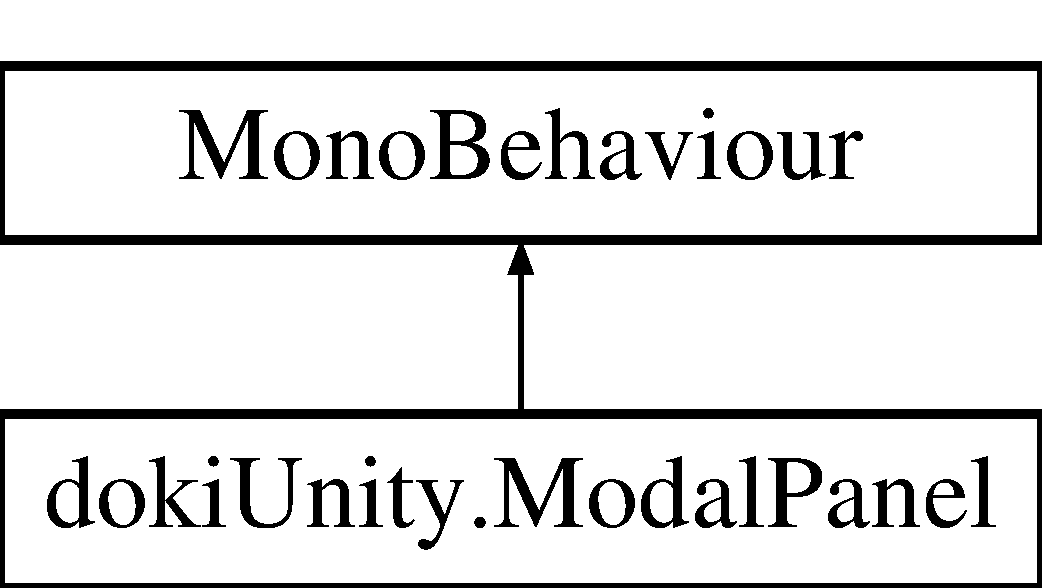
\includegraphics[height=2.000000cm]{classdoki_unity_1_1_modal_panel}
\end{center}
\end{figure}
\subsection*{Public Member Functions}
\begin{DoxyCompactItemize}
\item 
void \hyperlink{classdoki_unity_1_1_modal_panel_ab6e6c7b12989582f10d1947a52e20051}{Choice} (string title, string message, Unity\+Action$<$ bool $>$ yes\+Event)
\begin{DoxyCompactList}\small\item\em Show and customize the popup window\textquotesingle{}s title, message, yes\+Button\textquotesingle{}s callback function \end{DoxyCompactList}\item 
void \hyperlink{classdoki_unity_1_1_modal_panel_a919e94df42bca242808a093c3d06e5b4}{Choice} (string title, string message, Unity\+Action$<$ bool, System.\+Object $>$ yes\+Event, System.\+Object yes\+Parameter)
\begin{DoxyCompactList}\small\item\em Show and customize the popup window\textquotesingle{}s title, message, yes\+Button\textquotesingle{}s callback function and parameters should be passed to the function \end{DoxyCompactList}\item 
void \hyperlink{classdoki_unity_1_1_modal_panel_aa967d929957bd4a42663cbdb1ed4127f}{Choice} (string title, string message, Unity\+Action$<$ bool $>$ yes\+Event, Unity\+Action$<$ bool $>$ no\+Event)
\begin{DoxyCompactList}\small\item\em Show and customize the popup window\textquotesingle{}s title, message, yes\+Button\textquotesingle{}s callback function and no\+Button\textquotesingle{}s callback function \end{DoxyCompactList}\end{DoxyCompactItemize}
\subsection*{Public Attributes}
\begin{DoxyCompactItemize}
\item 
Text \hyperlink{classdoki_unity_1_1_modal_panel_a8bb32dc36292b9da60c7125f150d759d}{title\+Text}
\begin{DoxyCompactList}\small\item\em Pointer to the title\+Text Game\+Object \end{DoxyCompactList}\item 
Text \hyperlink{classdoki_unity_1_1_modal_panel_a6c9c26430055c5e6beb1d7db2dfb6f68}{message\+Text}
\begin{DoxyCompactList}\small\item\em Pointer to the message\+Text Game\+Object \end{DoxyCompactList}\item 
Button \hyperlink{classdoki_unity_1_1_modal_panel_a72113e073c692caa38601f17c6ffde6c}{yes\+Button}
\begin{DoxyCompactList}\small\item\em Pointer to the yes\+Button Game\+Object \end{DoxyCompactList}\item 
Button \hyperlink{classdoki_unity_1_1_modal_panel_ab383aea9285e694802836034b933f1f5}{no\+Button}
\begin{DoxyCompactList}\small\item\em Pointer to the no\+Button Game\+Object \end{DoxyCompactList}\end{DoxyCompactItemize}


\subsection{Detailed Description}
\hyperlink{classdoki_unity_1_1_modal_panel}{Modal\+Panel} is a template to create a pop up window to wait for player\textquotesingle{}s option input. \hyperlink{classdoki_unity_1_1_modal_panel}{Modal\+Panel} has a title, message, Yes button (and No button). External callback function could be passed to this window, and when responding button is clicked, the responding functions would be called. 



\subsection{Member Function Documentation}
\index{doki\+Unity\+::\+Modal\+Panel@{doki\+Unity\+::\+Modal\+Panel}!Choice@{Choice}}
\index{Choice@{Choice}!doki\+Unity\+::\+Modal\+Panel@{doki\+Unity\+::\+Modal\+Panel}}
\subsubsection[{\texorpdfstring{Choice(string title, string message, Unity\+Action$<$ bool $>$ yes\+Event)}{Choice(string title, string message, UnityAction< bool > yesEvent)}}]{\setlength{\rightskip}{0pt plus 5cm}void doki\+Unity.\+Modal\+Panel.\+Choice (
\begin{DoxyParamCaption}
\item[{string}]{title, }
\item[{string}]{message, }
\item[{Unity\+Action$<$ bool $>$}]{yes\+Event}
\end{DoxyParamCaption}
)}\hypertarget{classdoki_unity_1_1_modal_panel_ab6e6c7b12989582f10d1947a52e20051}{}\label{classdoki_unity_1_1_modal_panel_ab6e6c7b12989582f10d1947a52e20051}


Show and customize the popup window\textquotesingle{}s title, message, yes\+Button\textquotesingle{}s callback function 


\begin{DoxyParams}{Parameters}
{\em title} & Title of the window\\
\hline
{\em message} & Message insidethe window\\
\hline
{\em yes\+Event} & Callback function of yes\+Button\\
\hline
\end{DoxyParams}
\index{doki\+Unity\+::\+Modal\+Panel@{doki\+Unity\+::\+Modal\+Panel}!Choice@{Choice}}
\index{Choice@{Choice}!doki\+Unity\+::\+Modal\+Panel@{doki\+Unity\+::\+Modal\+Panel}}
\subsubsection[{\texorpdfstring{Choice(string title, string message, Unity\+Action$<$ bool, System.\+Object $>$ yes\+Event, System.\+Object yes\+Parameter)}{Choice(string title, string message, UnityAction< bool, System.Object > yesEvent, System.Object yesParameter)}}]{\setlength{\rightskip}{0pt plus 5cm}void doki\+Unity.\+Modal\+Panel.\+Choice (
\begin{DoxyParamCaption}
\item[{string}]{title, }
\item[{string}]{message, }
\item[{Unity\+Action$<$ bool, System.\+Object $>$}]{yes\+Event, }
\item[{System.\+Object}]{yes\+Parameter}
\end{DoxyParamCaption}
)}\hypertarget{classdoki_unity_1_1_modal_panel_a919e94df42bca242808a093c3d06e5b4}{}\label{classdoki_unity_1_1_modal_panel_a919e94df42bca242808a093c3d06e5b4}


Show and customize the popup window\textquotesingle{}s title, message, yes\+Button\textquotesingle{}s callback function and parameters should be passed to the function 


\begin{DoxyParams}{Parameters}
{\em title} & Title of the window\\
\hline
{\em message} & Message inside the window\\
\hline
{\em yes\+Event} & Callback function of yes\+Button\\
\hline
{\em yes\+Parameter} & Parameter should be passed to the yes\+Button\textquotesingle{}s callback function\\
\hline
\end{DoxyParams}
\index{doki\+Unity\+::\+Modal\+Panel@{doki\+Unity\+::\+Modal\+Panel}!Choice@{Choice}}
\index{Choice@{Choice}!doki\+Unity\+::\+Modal\+Panel@{doki\+Unity\+::\+Modal\+Panel}}
\subsubsection[{\texorpdfstring{Choice(string title, string message, Unity\+Action$<$ bool $>$ yes\+Event, Unity\+Action$<$ bool $>$ no\+Event)}{Choice(string title, string message, UnityAction< bool > yesEvent, UnityAction< bool > noEvent)}}]{\setlength{\rightskip}{0pt plus 5cm}void doki\+Unity.\+Modal\+Panel.\+Choice (
\begin{DoxyParamCaption}
\item[{string}]{title, }
\item[{string}]{message, }
\item[{Unity\+Action$<$ bool $>$}]{yes\+Event, }
\item[{Unity\+Action$<$ bool $>$}]{no\+Event}
\end{DoxyParamCaption}
)}\hypertarget{classdoki_unity_1_1_modal_panel_aa967d929957bd4a42663cbdb1ed4127f}{}\label{classdoki_unity_1_1_modal_panel_aa967d929957bd4a42663cbdb1ed4127f}


Show and customize the popup window\textquotesingle{}s title, message, yes\+Button\textquotesingle{}s callback function and no\+Button\textquotesingle{}s callback function 


\begin{DoxyParams}{Parameters}
{\em title} & Title of the window\\
\hline
{\em message} & Message inside the window\\
\hline
{\em yes\+Event} & Callback function of yes\+Button\\
\hline
{\em no\+Event} & Callback function of no\+Button\\
\hline
\end{DoxyParams}


\subsection{Member Data Documentation}
\index{doki\+Unity\+::\+Modal\+Panel@{doki\+Unity\+::\+Modal\+Panel}!message\+Text@{message\+Text}}
\index{message\+Text@{message\+Text}!doki\+Unity\+::\+Modal\+Panel@{doki\+Unity\+::\+Modal\+Panel}}
\subsubsection[{\texorpdfstring{message\+Text}{messageText}}]{\setlength{\rightskip}{0pt plus 5cm}Text doki\+Unity.\+Modal\+Panel.\+message\+Text}\hypertarget{classdoki_unity_1_1_modal_panel_a6c9c26430055c5e6beb1d7db2dfb6f68}{}\label{classdoki_unity_1_1_modal_panel_a6c9c26430055c5e6beb1d7db2dfb6f68}


Pointer to the message\+Text Game\+Object 

\index{doki\+Unity\+::\+Modal\+Panel@{doki\+Unity\+::\+Modal\+Panel}!no\+Button@{no\+Button}}
\index{no\+Button@{no\+Button}!doki\+Unity\+::\+Modal\+Panel@{doki\+Unity\+::\+Modal\+Panel}}
\subsubsection[{\texorpdfstring{no\+Button}{noButton}}]{\setlength{\rightskip}{0pt plus 5cm}Button doki\+Unity.\+Modal\+Panel.\+no\+Button}\hypertarget{classdoki_unity_1_1_modal_panel_ab383aea9285e694802836034b933f1f5}{}\label{classdoki_unity_1_1_modal_panel_ab383aea9285e694802836034b933f1f5}


Pointer to the no\+Button Game\+Object 

\index{doki\+Unity\+::\+Modal\+Panel@{doki\+Unity\+::\+Modal\+Panel}!title\+Text@{title\+Text}}
\index{title\+Text@{title\+Text}!doki\+Unity\+::\+Modal\+Panel@{doki\+Unity\+::\+Modal\+Panel}}
\subsubsection[{\texorpdfstring{title\+Text}{titleText}}]{\setlength{\rightskip}{0pt plus 5cm}Text doki\+Unity.\+Modal\+Panel.\+title\+Text}\hypertarget{classdoki_unity_1_1_modal_panel_a8bb32dc36292b9da60c7125f150d759d}{}\label{classdoki_unity_1_1_modal_panel_a8bb32dc36292b9da60c7125f150d759d}


Pointer to the title\+Text Game\+Object 

\index{doki\+Unity\+::\+Modal\+Panel@{doki\+Unity\+::\+Modal\+Panel}!yes\+Button@{yes\+Button}}
\index{yes\+Button@{yes\+Button}!doki\+Unity\+::\+Modal\+Panel@{doki\+Unity\+::\+Modal\+Panel}}
\subsubsection[{\texorpdfstring{yes\+Button}{yesButton}}]{\setlength{\rightskip}{0pt plus 5cm}Button doki\+Unity.\+Modal\+Panel.\+yes\+Button}\hypertarget{classdoki_unity_1_1_modal_panel_a72113e073c692caa38601f17c6ffde6c}{}\label{classdoki_unity_1_1_modal_panel_a72113e073c692caa38601f17c6ffde6c}


Pointer to the yes\+Button Game\+Object 



The documentation for this class was generated from the following file\+:\begin{DoxyCompactItemize}
\item 
C\+:/\+\_\+\+Projects/dokidoki/src/doki\+Unity/\+Assets/dokidoki/\+Scripts/\+U\+I\+Manager/Modal\+Panel.\+cs\end{DoxyCompactItemize}

\input{classdoki_unity_1_1_multiple_resolution_manager}
\hypertarget{classdoki_script_setting_1_1_namespace_doc}{}\section{doki\+Script\+Setting.\+Namespace\+Doc Class Reference}
\label{classdoki_script_setting_1_1_namespace_doc}\index{doki\+Script\+Setting.\+Namespace\+Doc@{doki\+Script\+Setting.\+Namespace\+Doc}}


The \hyperlink{namespacedoki_script_setting}{doki\+Script\+Setting} namespace contains classes for script setting about keywords, shared by \hyperlink{namespacedoki_unity}{doki\+Unity} and \hyperlink{namespacedoki_script_compiler}{doki\+Script\+Compiler}.  




\subsection{Detailed Description}
The \hyperlink{namespacedoki_script_setting}{doki\+Script\+Setting} namespace contains classes for script setting about keywords, shared by \hyperlink{namespacedoki_unity}{doki\+Unity} and \hyperlink{namespacedoki_script_compiler}{doki\+Script\+Compiler}. 



The documentation for this class was generated from the following file\+:\begin{DoxyCompactItemize}
\item 
C\+:/\+\_\+\+Projects/dokidoki/src/doki\+Script\+Setting/doki\+Script\+Setting/Namespace\+Doc.\+cs\end{DoxyCompactItemize}

\hypertarget{classdoki_battle_1_1_namespace_doc}{}\section{doki\+Battle.\+Namespace\+Doc Class Reference}
\label{classdoki_battle_1_1_namespace_doc}\index{doki\+Battle.\+Namespace\+Doc@{doki\+Battle.\+Namespace\+Doc}}


The \hyperlink{namespacedoki_battle}{doki\+Battle} namespace contains classes for turn-\/based battle.  




\subsection{Detailed Description}
The \hyperlink{namespacedoki_battle}{doki\+Battle} namespace contains classes for turn-\/based battle. 



The documentation for this class was generated from the following file\+:\begin{DoxyCompactItemize}
\item 
C\+:/\+\_\+\+Projects/dokidoki/src/doki\+Unity/\+Assets/dokidoki/\+Scripts/\+Battle/Namespace\+Doc.\+cs\end{DoxyCompactItemize}

\hypertarget{classdoki_script_compiler_1_1_namespace_doc}{}\section{doki\+Script\+Compiler.\+Namespace\+Doc Class Reference}
\label{classdoki_script_compiler_1_1_namespace_doc}\index{doki\+Script\+Compiler.\+Namespace\+Doc@{doki\+Script\+Compiler.\+Namespace\+Doc}}


The \hyperlink{namespacedoki_script_compiler}{doki\+Script\+Compiler} namespace contains classes for script compiling.  




\subsection{Detailed Description}
The \hyperlink{namespacedoki_script_compiler}{doki\+Script\+Compiler} namespace contains classes for script compiling. 



The documentation for this class was generated from the following file\+:\begin{DoxyCompactItemize}
\item 
C\+:/\+\_\+\+Projects/dokidoki/src/doki\+Script\+Compiler/doki\+Script/Namespace\+Doc.\+cs\end{DoxyCompactItemize}

\hypertarget{classdoki_unity_1_1_namespace_doc}{}\section{doki\+Unity.\+Namespace\+Doc Class Reference}
\label{classdoki_unity_1_1_namespace_doc}\index{doki\+Unity.\+Namespace\+Doc@{doki\+Unity.\+Namespace\+Doc}}


The \hyperlink{namespacedoki_unity}{doki\+Unity} namespace contains classes for effect part on Unity.  




\subsection{Detailed Description}
The \hyperlink{namespacedoki_unity}{doki\+Unity} namespace contains classes for effect part on Unity. 



The documentation for this class was generated from the following file\+:\begin{DoxyCompactItemize}
\item 
C\+:/\+\_\+\+Projects/dokidoki/src/doki\+Unity/\+Assets/dokidoki/\+Scripts/\+Game\+Entity/Namespace\+Doc.\+cs\end{DoxyCompactItemize}

\hypertarget{classdoki_script_setting_1_1_script}{}\section{doki\+Script\+Setting.\+Script Class Reference}
\label{classdoki_script_setting_1_1_script}\index{doki\+Script\+Setting.\+Script@{doki\+Script\+Setting.\+Script}}


\hyperlink{classdoki_script_setting_1_1_script}{Script} represents one script file which is compiled into an object. \hyperlink{classdoki_script_setting_1_1_script}{Script} is a set of Actions.  


\subsection*{Public Attributes}
\begin{DoxyCompactItemize}
\item 
List$<$ \hyperlink{classdoki_script_setting_1_1_action}{Action} $>$ \hyperlink{classdoki_script_setting_1_1_script_a7c04074aaeee592285f12d92718bea52}{actions}
\begin{DoxyCompactList}\small\item\em The list of actions compiled from script file \end{DoxyCompactList}\end{DoxyCompactItemize}


\subsection{Detailed Description}
\hyperlink{classdoki_script_setting_1_1_script}{Script} represents one script file which is compiled into an object. \hyperlink{classdoki_script_setting_1_1_script}{Script} is a set of Actions. 



\subsection{Member Data Documentation}
\index{doki\+Script\+Setting\+::\+Script@{doki\+Script\+Setting\+::\+Script}!actions@{actions}}
\index{actions@{actions}!doki\+Script\+Setting\+::\+Script@{doki\+Script\+Setting\+::\+Script}}
\subsubsection[{\texorpdfstring{actions}{actions}}]{\setlength{\rightskip}{0pt plus 5cm}List$<${\bf Action}$>$ doki\+Script\+Setting.\+Script.\+actions}\hypertarget{classdoki_script_setting_1_1_script_a7c04074aaeee592285f12d92718bea52}{}\label{classdoki_script_setting_1_1_script_a7c04074aaeee592285f12d92718bea52}


The list of actions compiled from script file 



The documentation for this class was generated from the following file\+:\begin{DoxyCompactItemize}
\item 
C\+:/\+\_\+\+Projects/dokidoki/src/doki\+Script\+Setting/doki\+Script\+Setting/Script.\+cs\end{DoxyCompactItemize}

\hypertarget{classdoki_script_setting_1_1_script_keyword}{}\section{doki\+Script\+Setting.\+Script\+Keyword Class Reference}
\label{classdoki_script_setting_1_1_script_keyword}\index{doki\+Script\+Setting.\+Script\+Keyword@{doki\+Script\+Setting.\+Script\+Keyword}}


\hyperlink{classdoki_script_setting_1_1_script_keyword}{Script\+Keyword} is the pre-\/defined related keywords of script  


\subsection*{Public Attributes}
\begin{DoxyCompactItemize}
\item 
const string {\bfseries S\+C\+R\+I\+P\+T\+\_\+\+E\+X\+T\+E\+N\+S\+I\+ON} = \char`\"{}dks\char`\"{}\hypertarget{classdoki_script_setting_1_1_script_keyword_a131141ba69563d9b6d3672b7904a7bf3}{}\label{classdoki_script_setting_1_1_script_keyword_a131141ba69563d9b6d3672b7904a7bf3}

\item 
const string {\bfseries S\+C\+R\+I\+P\+T\+\_\+\+C\+O\+M\+P\+I\+L\+E\+D\+\_\+\+E\+X\+T\+E\+N\+S\+I\+ON} = \char`\"{}txt\char`\"{}\hypertarget{classdoki_script_setting_1_1_script_keyword_a8499133323bfb65ad465f8dff32eee69}{}\label{classdoki_script_setting_1_1_script_keyword_a8499133323bfb65ad465f8dff32eee69}

\item 
const string {\bfseries W\+O\+R\+LD} = \char`\"{}world\char`\"{}\hypertarget{classdoki_script_setting_1_1_script_keyword_abc707d180df77142ce62c0044e58a2f0}{}\label{classdoki_script_setting_1_1_script_keyword_abc707d180df77142ce62c0044e58a2f0}

\item 
const string {\bfseries B\+A\+C\+K\+G\+R\+O\+U\+ND} = \char`\"{}background\char`\"{}\hypertarget{classdoki_script_setting_1_1_script_keyword_a71e98925fa468e7c5d732a1e5f78c7cd}{}\label{classdoki_script_setting_1_1_script_keyword_a71e98925fa468e7c5d732a1e5f78c7cd}

\item 
const string {\bfseries W\+E\+A\+T\+H\+ER} = \char`\"{}weather\char`\"{}\hypertarget{classdoki_script_setting_1_1_script_keyword_a461ac9dcc865863cd5a0a9bd0e2c216c}{}\label{classdoki_script_setting_1_1_script_keyword_a461ac9dcc865863cd5a0a9bd0e2c216c}

\item 
const string {\bfseries S\+O\+U\+ND} = \char`\"{}sound\char`\"{}\hypertarget{classdoki_script_setting_1_1_script_keyword_a7e62eee73a3a18dcf9a04c074a96f0f0}{}\label{classdoki_script_setting_1_1_script_keyword_a7e62eee73a3a18dcf9a04c074a96f0f0}

\item 
const string {\bfseries B\+GM} = \char`\"{}bgm\char`\"{}\hypertarget{classdoki_script_setting_1_1_script_keyword_a3b03fa39b41ea7a68e84c52dff3d7c84}{}\label{classdoki_script_setting_1_1_script_keyword_a3b03fa39b41ea7a68e84c52dff3d7c84}

\item 
const string {\bfseries V\+I\+D\+EO} = \char`\"{}video\char`\"{}\hypertarget{classdoki_script_setting_1_1_script_keyword_a5d5a64e71e4f6321253d327425dfd104}{}\label{classdoki_script_setting_1_1_script_keyword_a5d5a64e71e4f6321253d327425dfd104}

\item 
const string {\bfseries T\+E\+XT} = \char`\"{}text\char`\"{}\hypertarget{classdoki_script_setting_1_1_script_keyword_ab0b2f10604f07609238a4784a4711d9a}{}\label{classdoki_script_setting_1_1_script_keyword_ab0b2f10604f07609238a4784a4711d9a}

\item 
const string {\bfseries M\+O\+VE} = \char`\"{}move\char`\"{}\hypertarget{classdoki_script_setting_1_1_script_keyword_abb5921f802c476fd725edb95dfe56dd5}{}\label{classdoki_script_setting_1_1_script_keyword_abb5921f802c476fd725edb95dfe56dd5}

\item 
const string {\bfseries P\+O\+S\+T\+U\+RE} = \char`\"{}posture\char`\"{}\hypertarget{classdoki_script_setting_1_1_script_keyword_a498f9fd380985f17d8a4e3252f0b1fcf}{}\label{classdoki_script_setting_1_1_script_keyword_a498f9fd380985f17d8a4e3252f0b1fcf}

\item 
const string {\bfseries F\+A\+CE} = \char`\"{}face\char`\"{}\hypertarget{classdoki_script_setting_1_1_script_keyword_aba5a252e70358164aa5fcab43164ca85}{}\label{classdoki_script_setting_1_1_script_keyword_aba5a252e70358164aa5fcab43164ca85}

\item 
const string {\bfseries V\+O\+I\+CE} = \char`\"{}voice\char`\"{}\hypertarget{classdoki_script_setting_1_1_script_keyword_a719fdafadbf0fa22061aba4d44054935}{}\label{classdoki_script_setting_1_1_script_keyword_a719fdafadbf0fa22061aba4d44054935}

\item 
const string {\bfseries R\+O\+LE} = \char`\"{}role\char`\"{}\hypertarget{classdoki_script_setting_1_1_script_keyword_a506107047245e3f05da2878529e0aa1b}{}\label{classdoki_script_setting_1_1_script_keyword_a506107047245e3f05da2878529e0aa1b}

\item 
const string {\bfseries F\+O\+C\+US} = \char`\"{}focus\char`\"{}\hypertarget{classdoki_script_setting_1_1_script_keyword_a388a9ae97322638b948fdd3614ae0029}{}\label{classdoki_script_setting_1_1_script_keyword_a388a9ae97322638b948fdd3614ae0029}

\item 
const string {\bfseries F\+L\+AG} = \char`\"{}flag\char`\"{}\hypertarget{classdoki_script_setting_1_1_script_keyword_a880caa3a8bbdd9003df63b7db4da8e05}{}\label{classdoki_script_setting_1_1_script_keyword_a880caa3a8bbdd9003df63b7db4da8e05}

\item 
const string {\bfseries O\+P\+T\+I\+ON} = \char`\"{}option\char`\"{}\hypertarget{classdoki_script_setting_1_1_script_keyword_a325eb7cbc49349b257c6aaaa4d159105}{}\label{classdoki_script_setting_1_1_script_keyword_a325eb7cbc49349b257c6aaaa4d159105}

\item 
const string {\bfseries J\+U\+MP} = \char`\"{}jump\char`\"{}\hypertarget{classdoki_script_setting_1_1_script_keyword_a44dda5a642a58af9fb4bd1f643a5d342}{}\label{classdoki_script_setting_1_1_script_keyword_a44dda5a642a58af9fb4bd1f643a5d342}

\item 
const string {\bfseries S\+RC} = \char`\"{}src\char`\"{}\hypertarget{classdoki_script_setting_1_1_script_keyword_a9453a82013a702f2ed0e391dfd6d0684}{}\label{classdoki_script_setting_1_1_script_keyword_a9453a82013a702f2ed0e391dfd6d0684}

\item 
const string {\bfseries T\+R\+A\+N\+S\+I\+T\+I\+ON} = \char`\"{}transition\char`\"{}\hypertarget{classdoki_script_setting_1_1_script_keyword_a3e27767fa5bbc9eca778a36fbb1fc80a}{}\label{classdoki_script_setting_1_1_script_keyword_a3e27767fa5bbc9eca778a36fbb1fc80a}

\item 
const string {\bfseries T\+R\+A\+N\+S\+I\+T\+I\+O\+N\+\_\+\+I\+N\+S\+T\+A\+NT} = \char`\"{}instant\char`\"{}\hypertarget{classdoki_script_setting_1_1_script_keyword_a6999d890bf952f54241b085b01fdba7d}{}\label{classdoki_script_setting_1_1_script_keyword_a6999d890bf952f54241b085b01fdba7d}

\item 
const string {\bfseries T\+R\+A\+N\+S\+I\+T\+I\+O\+N\+\_\+\+G\+R\+A\+D\+U\+AL} = \char`\"{}gradual\char`\"{}\hypertarget{classdoki_script_setting_1_1_script_keyword_a11539e084d719bace9ba0b66714cd713}{}\label{classdoki_script_setting_1_1_script_keyword_a11539e084d719bace9ba0b66714cd713}

\item 
const string {\bfseries S\+P\+E\+ED} = \char`\"{}speed\char`\"{}\hypertarget{classdoki_script_setting_1_1_script_keyword_a1475821c8a547baea9a4235e7274606e}{}\label{classdoki_script_setting_1_1_script_keyword_a1475821c8a547baea9a4235e7274606e}

\item 
const string {\bfseries T\+Y\+PE} = \char`\"{}type\char`\"{}\hypertarget{classdoki_script_setting_1_1_script_keyword_a25323bf4996d047578ae2f9c10dab9e4}{}\label{classdoki_script_setting_1_1_script_keyword_a25323bf4996d047578ae2f9c10dab9e4}

\item 
const string {\bfseries T\+Y\+P\+E\+\_\+\+S\+U\+N\+NY} = \char`\"{}sunny\char`\"{}\hypertarget{classdoki_script_setting_1_1_script_keyword_a08b99303a09ee2550ef8bfeb7a62cfd6}{}\label{classdoki_script_setting_1_1_script_keyword_a08b99303a09ee2550ef8bfeb7a62cfd6}

\item 
const string {\bfseries T\+Y\+P\+E\+\_\+\+C\+L\+O\+U\+DY} = \char`\"{}cloudy\char`\"{}\hypertarget{classdoki_script_setting_1_1_script_keyword_ae450070c4c3ed2e437efdf1b7701c2d8}{}\label{classdoki_script_setting_1_1_script_keyword_ae450070c4c3ed2e437efdf1b7701c2d8}

\item 
const string {\bfseries T\+Y\+P\+E\+\_\+\+R\+A\+IN} = \char`\"{}rain\char`\"{}\hypertarget{classdoki_script_setting_1_1_script_keyword_a447dbb0df50e74172536ad0cce23783f}{}\label{classdoki_script_setting_1_1_script_keyword_a447dbb0df50e74172536ad0cce23783f}

\item 
const string {\bfseries T\+Y\+P\+E\+\_\+\+S\+N\+OW} = \char`\"{}snow\char`\"{}\hypertarget{classdoki_script_setting_1_1_script_keyword_a519a5fb7c260049c68f7bbe44f41ffbd}{}\label{classdoki_script_setting_1_1_script_keyword_a519a5fb7c260049c68f7bbe44f41ffbd}

\item 
const string {\bfseries L\+E\+V\+EL} = \char`\"{}level\char`\"{}\hypertarget{classdoki_script_setting_1_1_script_keyword_aeaa3c47953e7766586fc4db2dc9ef79a}{}\label{classdoki_script_setting_1_1_script_keyword_aeaa3c47953e7766586fc4db2dc9ef79a}

\item 
const string {\bfseries M\+O\+DE} = \char`\"{}mode\char`\"{}\hypertarget{classdoki_script_setting_1_1_script_keyword_a29b81ec572a0bdfbe24c9aded3e9d7da}{}\label{classdoki_script_setting_1_1_script_keyword_a29b81ec572a0bdfbe24c9aded3e9d7da}

\item 
const string {\bfseries M\+O\+D\+E\+\_\+\+L\+O\+OP} = \char`\"{}loop\char`\"{}\hypertarget{classdoki_script_setting_1_1_script_keyword_a52d7d7308106bd733fab65ec0816b8e4}{}\label{classdoki_script_setting_1_1_script_keyword_a52d7d7308106bd733fab65ec0816b8e4}

\item 
const string {\bfseries C\+O\+N\+T\+E\+NT} = \char`\"{}content\char`\"{}\hypertarget{classdoki_script_setting_1_1_script_keyword_af2d0488f7bca2e12b7f20d4e6cd39db3}{}\label{classdoki_script_setting_1_1_script_keyword_af2d0488f7bca2e12b7f20d4e6cd39db3}

\item 
const string {\bfseries P\+O\+S\+I\+T\+I\+ON} = \char`\"{}position\char`\"{}\hypertarget{classdoki_script_setting_1_1_script_keyword_ae2edc8dc6841dca4ab3168ce900e7784}{}\label{classdoki_script_setting_1_1_script_keyword_ae2edc8dc6841dca4ab3168ce900e7784}

\item 
const string {\bfseries P\+O\+S\+I\+T\+I\+O\+N\+\_\+\+C\+E\+N\+T\+ER} = \char`\"{}center\char`\"{}\hypertarget{classdoki_script_setting_1_1_script_keyword_a665deb03da5e51606e7fde2ebe1ff929}{}\label{classdoki_script_setting_1_1_script_keyword_a665deb03da5e51606e7fde2ebe1ff929}

\item 
const string {\bfseries P\+O\+S\+I\+T\+I\+O\+N\+\_\+\+L\+E\+FT} = \char`\"{}left\char`\"{}\hypertarget{classdoki_script_setting_1_1_script_keyword_afec688036841831b2b0e8cd33db73581}{}\label{classdoki_script_setting_1_1_script_keyword_afec688036841831b2b0e8cd33db73581}

\item 
const string {\bfseries P\+O\+S\+I\+T\+I\+O\+N\+\_\+\+R\+I\+G\+HT} = \char`\"{}right\char`\"{}\hypertarget{classdoki_script_setting_1_1_script_keyword_a23aebe6588a787f336495fa3f874efa9}{}\label{classdoki_script_setting_1_1_script_keyword_a23aebe6588a787f336495fa3f874efa9}

\item 
const string {\bfseries A\+N\+C\+H\+OR} =\char`\"{}anchor\char`\"{}\hypertarget{classdoki_script_setting_1_1_script_keyword_a7a95701ddcb34fff80d7fd0b33b8684a}{}\label{classdoki_script_setting_1_1_script_keyword_a7a95701ddcb34fff80d7fd0b33b8684a}

\item 
const string {\bfseries T\+Y\+P\+E\+\_\+\+P\+L\+A\+Y\+ER} = \char`\"{}player\char`\"{}\hypertarget{classdoki_script_setting_1_1_script_keyword_ac9fcd6e299c785d91211f083e7da594e}{}\label{classdoki_script_setting_1_1_script_keyword_ac9fcd6e299c785d91211f083e7da594e}

\item 
const string {\bfseries T\+Y\+P\+E\+\_\+\+C\+H\+A\+R\+A\+C\+T\+ER} = \char`\"{}character\char`\"{}\hypertarget{classdoki_script_setting_1_1_script_keyword_ab860152dff9286d6d63d3e97326d1d3d}{}\label{classdoki_script_setting_1_1_script_keyword_ab860152dff9286d6d63d3e97326d1d3d}

\item 
const string {\bfseries N\+A\+ME} = \char`\"{}name\char`\"{}\hypertarget{classdoki_script_setting_1_1_script_keyword_ac75a893cc668e947e909ee48a3a34bf3}{}\label{classdoki_script_setting_1_1_script_keyword_ac75a893cc668e947e909ee48a3a34bf3}

\item 
const string {\bfseries ID} = \char`\"{}id\char`\"{}\hypertarget{classdoki_script_setting_1_1_script_keyword_a73e6a9369ef0206700658580f4d094b5}{}\label{classdoki_script_setting_1_1_script_keyword_a73e6a9369ef0206700658580f4d094b5}

\item 
const string {\bfseries C\+O\+U\+NT} = \char`\"{}count\char`\"{}\hypertarget{classdoki_script_setting_1_1_script_keyword_a557cb5ea096913b156f203f6005dd14a}{}\label{classdoki_script_setting_1_1_script_keyword_a557cb5ea096913b156f203f6005dd14a}

\item 
const string {\bfseries O\+P\+T\+I\+O\+N\+\_\+} = \char`\"{}option\char`\"{}\hypertarget{classdoki_script_setting_1_1_script_keyword_a82eaf58d7bdf1261c2a6064ad18bb0eb}{}\label{classdoki_script_setting_1_1_script_keyword_a82eaf58d7bdf1261c2a6064ad18bb0eb}

\item 
const string {\bfseries O\+P\+T\+I\+O\+N\+\_\+\+I\+D\+\_\+} = \char`\"{}option\+Id\char`\"{}\hypertarget{classdoki_script_setting_1_1_script_keyword_aa8049c8a08ffaae34a99d5517adab4f2}{}\label{classdoki_script_setting_1_1_script_keyword_aa8049c8a08ffaae34a99d5517adab4f2}

\item 
const string {\bfseries O\+P\+T\+I\+O\+N\+\_\+\+S\+R\+C\+\_\+} = \char`\"{}option\+Src\char`\"{}\hypertarget{classdoki_script_setting_1_1_script_keyword_a9b0fe349b6401051e3294662b4b559d2}{}\label{classdoki_script_setting_1_1_script_keyword_a9b0fe349b6401051e3294662b4b559d2}

\item 
const string {\bfseries O\+P\+T\+I\+O\+N\+\_\+1} = \char`\"{}option1\char`\"{}\hypertarget{classdoki_script_setting_1_1_script_keyword_aabedbba29ac7a465ff062755c4a4bf68}{}\label{classdoki_script_setting_1_1_script_keyword_aabedbba29ac7a465ff062755c4a4bf68}

\item 
const string {\bfseries O\+P\+T\+I\+O\+N\+\_\+\+I\+D\+\_\+1} = \char`\"{}option\+Id1\char`\"{}\hypertarget{classdoki_script_setting_1_1_script_keyword_af2e05234e3ea427056f454ab768e4ba1}{}\label{classdoki_script_setting_1_1_script_keyword_af2e05234e3ea427056f454ab768e4ba1}

\item 
const string {\bfseries O\+P\+T\+I\+O\+N\+\_\+\+S\+R\+C\+\_\+1} = \char`\"{}option\+Src1\char`\"{}\hypertarget{classdoki_script_setting_1_1_script_keyword_a6d5e264860c25ce0e929794aae8515e8}{}\label{classdoki_script_setting_1_1_script_keyword_a6d5e264860c25ce0e929794aae8515e8}

\item 
const string {\bfseries O\+P\+T\+I\+O\+N\+\_\+2} = \char`\"{}option2\char`\"{}\hypertarget{classdoki_script_setting_1_1_script_keyword_a33ad227f70a61d2dda8653dee55d48de}{}\label{classdoki_script_setting_1_1_script_keyword_a33ad227f70a61d2dda8653dee55d48de}

\item 
const string {\bfseries O\+P\+T\+I\+O\+N\+\_\+\+I\+D\+\_\+2} = \char`\"{}option\+Id2\char`\"{}\hypertarget{classdoki_script_setting_1_1_script_keyword_aeac21f75f5781e336492eb60e7e6e28c}{}\label{classdoki_script_setting_1_1_script_keyword_aeac21f75f5781e336492eb60e7e6e28c}

\item 
const string {\bfseries O\+P\+T\+I\+O\+N\+\_\+\+S\+R\+C\+\_\+2} = \char`\"{}option\+Src2\char`\"{}\hypertarget{classdoki_script_setting_1_1_script_keyword_af0442e4b48d4d3d409098436e666fbc1}{}\label{classdoki_script_setting_1_1_script_keyword_af0442e4b48d4d3d409098436e666fbc1}

\item 
const string {\bfseries O\+P\+T\+I\+O\+N\+\_\+3} = \char`\"{}option3\char`\"{}\hypertarget{classdoki_script_setting_1_1_script_keyword_a1876dcb6ffc3faaa7b6f5e7c33a7050a}{}\label{classdoki_script_setting_1_1_script_keyword_a1876dcb6ffc3faaa7b6f5e7c33a7050a}

\item 
const string {\bfseries O\+P\+T\+I\+O\+N\+\_\+\+I\+D\+\_\+3} = \char`\"{}option\+Id3\char`\"{}\hypertarget{classdoki_script_setting_1_1_script_keyword_a54dcd8b074d0a25f7a47166d02e056e6}{}\label{classdoki_script_setting_1_1_script_keyword_a54dcd8b074d0a25f7a47166d02e056e6}

\item 
const string {\bfseries O\+P\+T\+I\+O\+N\+\_\+\+S\+R\+C\+\_\+3} = \char`\"{}option\+Src3\char`\"{}\hypertarget{classdoki_script_setting_1_1_script_keyword_a62ab8e8e42d4c889f88a0c784845b9f2}{}\label{classdoki_script_setting_1_1_script_keyword_a62ab8e8e42d4c889f88a0c784845b9f2}

\item 
const string {\bfseries O\+P\+T\+I\+O\+N\+\_\+4} = \char`\"{}option4\char`\"{}\hypertarget{classdoki_script_setting_1_1_script_keyword_a7107b73879057d8f96a701d9914c0af1}{}\label{classdoki_script_setting_1_1_script_keyword_a7107b73879057d8f96a701d9914c0af1}

\item 
const string {\bfseries O\+P\+T\+I\+O\+N\+\_\+\+I\+D\+\_\+4} = \char`\"{}option\+Id4\char`\"{}\hypertarget{classdoki_script_setting_1_1_script_keyword_a49b2c05812b919ea7b6a6c367d36be40}{}\label{classdoki_script_setting_1_1_script_keyword_a49b2c05812b919ea7b6a6c367d36be40}

\item 
const string {\bfseries O\+P\+T\+I\+O\+N\+\_\+\+S\+R\+C\+\_\+4} = \char`\"{}option\+Src4\char`\"{}\hypertarget{classdoki_script_setting_1_1_script_keyword_accb046057a578d255e6f4cd8380992e3}{}\label{classdoki_script_setting_1_1_script_keyword_accb046057a578d255e6f4cd8380992e3}

\item 
const string {\bfseries O\+P\+T\+I\+O\+N\+\_\+5} = \char`\"{}option5\char`\"{}\hypertarget{classdoki_script_setting_1_1_script_keyword_a3d9f2c814874fe746bc33551f4961ea1}{}\label{classdoki_script_setting_1_1_script_keyword_a3d9f2c814874fe746bc33551f4961ea1}

\item 
const string {\bfseries O\+P\+T\+I\+O\+N\+\_\+\+I\+D\+\_\+5} = \char`\"{}option\+Id5\char`\"{}\hypertarget{classdoki_script_setting_1_1_script_keyword_af89b3f1f3698e405a22bf7e4f5224d1b}{}\label{classdoki_script_setting_1_1_script_keyword_af89b3f1f3698e405a22bf7e4f5224d1b}

\item 
const string {\bfseries O\+P\+T\+I\+O\+N\+\_\+\+S\+R\+C\+\_\+5} = \char`\"{}option\+Src5\char`\"{}\hypertarget{classdoki_script_setting_1_1_script_keyword_a8ddfdd32bbf570d25e6bedee699b62db}{}\label{classdoki_script_setting_1_1_script_keyword_a8ddfdd32bbf570d25e6bedee699b62db}

\item 
const string {\bfseries O\+P\+T\+I\+O\+N\+\_\+6} = \char`\"{}option6\char`\"{}\hypertarget{classdoki_script_setting_1_1_script_keyword_ac8a66042c823b37fcf00fb8a237482f1}{}\label{classdoki_script_setting_1_1_script_keyword_ac8a66042c823b37fcf00fb8a237482f1}

\item 
const string {\bfseries O\+P\+T\+I\+O\+N\+\_\+\+I\+D\+\_\+6} = \char`\"{}option\+Id6\char`\"{}\hypertarget{classdoki_script_setting_1_1_script_keyword_a133f2479d82ffd87c9e419f40bfb28de}{}\label{classdoki_script_setting_1_1_script_keyword_a133f2479d82ffd87c9e419f40bfb28de}

\item 
const string {\bfseries O\+P\+T\+I\+O\+N\+\_\+\+S\+R\+C\+\_\+6} = \char`\"{}option\+Src6\char`\"{}\hypertarget{classdoki_script_setting_1_1_script_keyword_abf0087b7b5b0941675ae02d4ba821fdc}{}\label{classdoki_script_setting_1_1_script_keyword_abf0087b7b5b0941675ae02d4ba821fdc}

\item 
const string {\bfseries O\+P\+T\+I\+O\+N\+\_\+7} = \char`\"{}option7\char`\"{}\hypertarget{classdoki_script_setting_1_1_script_keyword_ac5602fb44ae083397c7704337de130bc}{}\label{classdoki_script_setting_1_1_script_keyword_ac5602fb44ae083397c7704337de130bc}

\item 
const string {\bfseries O\+P\+T\+I\+O\+N\+\_\+\+I\+D\+\_\+7} = \char`\"{}option\+Id7\char`\"{}\hypertarget{classdoki_script_setting_1_1_script_keyword_ab5f3524ea97b93597209ef99d5a7d83f}{}\label{classdoki_script_setting_1_1_script_keyword_ab5f3524ea97b93597209ef99d5a7d83f}

\item 
const string {\bfseries O\+P\+T\+I\+O\+N\+\_\+\+S\+R\+C\+\_\+7} = \char`\"{}option\+Src7\char`\"{}\hypertarget{classdoki_script_setting_1_1_script_keyword_a90aa500d673e824be233acccc242e04c}{}\label{classdoki_script_setting_1_1_script_keyword_a90aa500d673e824be233acccc242e04c}

\item 
const string {\bfseries O\+P\+T\+I\+O\+N\+\_\+8} = \char`\"{}option8\char`\"{}\hypertarget{classdoki_script_setting_1_1_script_keyword_ad14221c177f9610352872eb1e2950303}{}\label{classdoki_script_setting_1_1_script_keyword_ad14221c177f9610352872eb1e2950303}

\item 
const string {\bfseries O\+P\+T\+I\+O\+N\+\_\+\+I\+D\+\_\+8} = \char`\"{}option\+Id8\char`\"{}\hypertarget{classdoki_script_setting_1_1_script_keyword_a5fc8ea6274899c504aba92c13da50f6a}{}\label{classdoki_script_setting_1_1_script_keyword_a5fc8ea6274899c504aba92c13da50f6a}

\item 
const string {\bfseries O\+P\+T\+I\+O\+N\+\_\+\+S\+R\+C\+\_\+8} = \char`\"{}option\+Src8\char`\"{}\hypertarget{classdoki_script_setting_1_1_script_keyword_a04e12f02358352cbb655f2b42c136723}{}\label{classdoki_script_setting_1_1_script_keyword_a04e12f02358352cbb655f2b42c136723}

\item 
const string {\bfseries O\+P\+T\+I\+O\+N\+\_\+9} = \char`\"{}option9\char`\"{}\hypertarget{classdoki_script_setting_1_1_script_keyword_a623cf2bafa757d64c4562e7b21a10f0e}{}\label{classdoki_script_setting_1_1_script_keyword_a623cf2bafa757d64c4562e7b21a10f0e}

\item 
const string {\bfseries O\+P\+T\+I\+O\+N\+\_\+\+I\+D\+\_\+9} = \char`\"{}option\+Id9\char`\"{}\hypertarget{classdoki_script_setting_1_1_script_keyword_a9fe99687266e88dd8f999a3044772325}{}\label{classdoki_script_setting_1_1_script_keyword_a9fe99687266e88dd8f999a3044772325}

\item 
const string {\bfseries O\+P\+T\+I\+O\+N\+\_\+\+S\+R\+C\+\_\+9} = \char`\"{}option\+Src9\char`\"{}\hypertarget{classdoki_script_setting_1_1_script_keyword_a7727668b596ed5438ad2cd1e87f932dd}{}\label{classdoki_script_setting_1_1_script_keyword_a7727668b596ed5438ad2cd1e87f932dd}

\item 
const string {\bfseries B\+R\+A\+C\+K\+E\+T\+\_\+\+L\+E\+FT} = \char`\"{}\{\char`\"{}\hypertarget{classdoki_script_setting_1_1_script_keyword_af46f40eb223861b398bd76cb91ee8ae5}{}\label{classdoki_script_setting_1_1_script_keyword_af46f40eb223861b398bd76cb91ee8ae5}

\item 
const string {\bfseries B\+R\+A\+C\+K\+E\+T\+\_\+\+R\+I\+G\+HT} = \char`\"{}\}\char`\"{}\hypertarget{classdoki_script_setting_1_1_script_keyword_a9d1352346f3e65ae915709d1fe209aac}{}\label{classdoki_script_setting_1_1_script_keyword_a9d1352346f3e65ae915709d1fe209aac}

\item 
const string {\bfseries S\+Q\+U\+A\+R\+E\+\_\+\+B\+R\+A\+C\+K\+E\+T\+\_\+\+L\+E\+FT} = \char`\"{}\mbox{[}\char`\"{}\hypertarget{classdoki_script_setting_1_1_script_keyword_a7896ac75f410c02994d88c3f5ddd1e3b}{}\label{classdoki_script_setting_1_1_script_keyword_a7896ac75f410c02994d88c3f5ddd1e3b}

\item 
const string {\bfseries S\+Q\+U\+A\+R\+E\+\_\+\+B\+R\+A\+C\+K\+E\+T\+\_\+\+R\+I\+G\+HT} = \char`\"{}\mbox{]}\char`\"{}\hypertarget{classdoki_script_setting_1_1_script_keyword_a71e65e1b0333dfdea1449a04106b7c92}{}\label{classdoki_script_setting_1_1_script_keyword_a71e65e1b0333dfdea1449a04106b7c92}

\item 
const string {\bfseries P\+A\+R\+E\+N\+T\+H\+E\+S\+E\+\_\+\+L\+E\+FT} = \char`\"{}(\char`\"{}\hypertarget{classdoki_script_setting_1_1_script_keyword_a4532611da5b487c0ebe69b5389190ae5}{}\label{classdoki_script_setting_1_1_script_keyword_a4532611da5b487c0ebe69b5389190ae5}

\item 
const string {\bfseries P\+A\+R\+E\+N\+T\+H\+E\+S\+E\+\_\+\+R\+I\+G\+HT} = \char`\"{})\char`\"{}\hypertarget{classdoki_script_setting_1_1_script_keyword_aab4ffb4e722ca7696ccddd99fb2a9f9e}{}\label{classdoki_script_setting_1_1_script_keyword_aab4ffb4e722ca7696ccddd99fb2a9f9e}

\item 
const string {\bfseries A\+N\+G\+L\+E\+\_\+\+B\+R\+A\+C\+K\+E\+T\+\_\+\+L\+E\+FT} = \char`\"{}$<$\char`\"{}\hypertarget{classdoki_script_setting_1_1_script_keyword_a354045a9c0c919377a0307dc8ecd5ae8}{}\label{classdoki_script_setting_1_1_script_keyword_a354045a9c0c919377a0307dc8ecd5ae8}

\item 
const string {\bfseries D\+O\+U\+B\+L\+E\+\_\+\+Q\+U\+O\+TE} = \char`\"{}\textbackslash{}\char`\"{}\char`\"{}\hypertarget{classdoki_script_setting_1_1_script_keyword_a8fe2bd6a864ca6ee11e7abc423474635}{}\label{classdoki_script_setting_1_1_script_keyword_a8fe2bd6a864ca6ee11e7abc423474635}

\item 
const string {\bfseries P\+E\+R\+I\+OD} = \char`\"{}.\char`\"{}\hypertarget{classdoki_script_setting_1_1_script_keyword_a8225c8f2dd553b50a49316d8969f48df}{}\label{classdoki_script_setting_1_1_script_keyword_a8225c8f2dd553b50a49316d8969f48df}

\item 
const string {\bfseries C\+O\+M\+MA} = \char`\"{},\char`\"{}\hypertarget{classdoki_script_setting_1_1_script_keyword_a57cd7dc3e5ee31e44bb164b8ad629c61}{}\label{classdoki_script_setting_1_1_script_keyword_a57cd7dc3e5ee31e44bb164b8ad629c61}

\item 
const string {\bfseries S\+E\+M\+I\+C\+O\+L\+ON} = \char`\"{};\char`\"{}\hypertarget{classdoki_script_setting_1_1_script_keyword_a4dc969a8b7c20a58a52a0258984834f4}{}\label{classdoki_script_setting_1_1_script_keyword_a4dc969a8b7c20a58a52a0258984834f4}

\item 
const string {\bfseries E\+Q\+U\+AL} = \char`\"{}=\char`\"{}\hypertarget{classdoki_script_setting_1_1_script_keyword_a1bc3d9fb15dad5a50d66d1dc2f22252e}{}\label{classdoki_script_setting_1_1_script_keyword_a1bc3d9fb15dad5a50d66d1dc2f22252e}

\item 
const string {\bfseries C\+L\+I\+CK} = \char`\"{}$>$\char`\"{}\hypertarget{classdoki_script_setting_1_1_script_keyword_ada7804afea0354eec869fa65e2cae3cb}{}\label{classdoki_script_setting_1_1_script_keyword_ada7804afea0354eec869fa65e2cae3cb}

\item 
const string {\bfseries C\+L\+I\+C\+K\+\_\+\+N\+E\+X\+T\+\_\+\+D\+I\+A\+L\+O\+G\+U\+E\+\_\+\+P\+A\+GE} = \char`\"{}$>$$>$\char`\"{}\hypertarget{classdoki_script_setting_1_1_script_keyword_a531a92ce586fa5c5076da7021d05c3b7}{}\label{classdoki_script_setting_1_1_script_keyword_a531a92ce586fa5c5076da7021d05c3b7}

\item 
const string {\bfseries S\+T\+R\+I\+NG} = \char`\"{}\textbackslash{}\char`\"{}\char`\"{}\hypertarget{classdoki_script_setting_1_1_script_keyword_a231de469c928469961ab28120eed5182}{}\label{classdoki_script_setting_1_1_script_keyword_a231de469c928469961ab28120eed5182}

\item 
const string {\bfseries T\+AB} = \char`\"{}\textbackslash{}t\char`\"{}\hypertarget{classdoki_script_setting_1_1_script_keyword_a3100b9214df58e274aba0b04b8429aba}{}\label{classdoki_script_setting_1_1_script_keyword_a3100b9214df58e274aba0b04b8429aba}

\item 
const string {\bfseries E\+N\+T\+ER} = \char`\"{}\textbackslash{}n\char`\"{}\hypertarget{classdoki_script_setting_1_1_script_keyword_acf29e843788dbcf2e32c777c740192d4}{}\label{classdoki_script_setting_1_1_script_keyword_acf29e843788dbcf2e32c777c740192d4}

\item 
const string {\bfseries C\+O\+M\+M\+E\+NT} = \char`\"{}//\char`\"{}\hypertarget{classdoki_script_setting_1_1_script_keyword_a802a0dec6b9c0a30199f49a3e5aa72e6}{}\label{classdoki_script_setting_1_1_script_keyword_a802a0dec6b9c0a30199f49a3e5aa72e6}

\item 
const string {\bfseries C\+O\+M\+M\+E\+N\+T\+\_\+\+S\+T\+A\+RT} = \char`\"{}/$\ast$\char`\"{}\hypertarget{classdoki_script_setting_1_1_script_keyword_ad535b41caa80404a1b50228707f82d82}{}\label{classdoki_script_setting_1_1_script_keyword_ad535b41caa80404a1b50228707f82d82}

\item 
const string {\bfseries C\+O\+M\+M\+E\+N\+T\+\_\+\+E\+ND} = \char`\"{}$\ast$/\char`\"{}\hypertarget{classdoki_script_setting_1_1_script_keyword_a7c817fd69b607a33b86e13a695941a3f}{}\label{classdoki_script_setting_1_1_script_keyword_a7c817fd69b607a33b86e13a695941a3f}

\item 
const string {\bfseries A\+S\+S\+I\+GN} = \char`\"{}=\char`\"{}\hypertarget{classdoki_script_setting_1_1_script_keyword_a14593305d54e6d73765c3002fa37def3}{}\label{classdoki_script_setting_1_1_script_keyword_a14593305d54e6d73765c3002fa37def3}

\item 
const string {\bfseries OR} = \char`\"{}$\vert$\char`\"{}\hypertarget{classdoki_script_setting_1_1_script_keyword_ac992cc4cc624a056ee5aa6bd0848827d}{}\label{classdoki_script_setting_1_1_script_keyword_ac992cc4cc624a056ee5aa6bd0848827d}

\end{DoxyCompactItemize}


\subsection{Detailed Description}
\hyperlink{classdoki_script_setting_1_1_script_keyword}{Script\+Keyword} is the pre-\/defined related keywords of script 



The documentation for this class was generated from the following file\+:\begin{DoxyCompactItemize}
\item 
C\+:/\+\_\+\+Projects/dokidoki/src/doki\+Script\+Setting/doki\+Script\+Setting/Script\+Keyword.\+cs\end{DoxyCompactItemize}

\hypertarget{classdoki_unity_1_1_script_reader}{}\section{doki\+Unity.\+Script\+Reader Class Reference}
\label{classdoki_unity_1_1_script_reader}\index{doki\+Unity.\+Script\+Reader@{doki\+Unity.\+Script\+Reader}}


\hyperlink{classdoki_unity_1_1_script_reader}{Script\+Reader} is resiponsible for all script relating operations during the game. \hyperlink{classdoki_unity_1_1_script_reader}{Script\+Reader} could automatically search all scripts under the pre-\/defined folder(asset/\+Resources/\+Doki\+Scripts), and sort it in alphabet order. When a new game starts up, the first script would be loaded, and \hyperlink{classdoki_unity_1_1_script_reader}{Script\+Reader} keeps all Actions. When loads a game from saved data, the script with specific name would be loaded. A script is a set of actions. Those actions would be returned to \hyperlink{classdoki_unity_1_1_world_control}{World\+Control} to distribute them to \hyperlink{classdoki_unity_1_1_world}{World} or \hyperlink{classdoki_unity_1_1_character}{Character} to take in sequence.  


\subsection*{Public Member Functions}
\begin{DoxyCompactItemize}
\item 
\hyperlink{classdoki_unity_1_1_script_reader_a160a5172d896f0bdf7730e0500bb1bb2}{Script\+Reader} ()
\begin{DoxyCompactList}\small\item\em When script\+Read is new created, automatically searchs scripts \end{DoxyCompactList}\item 
List$<$ \hyperlink{classdoki_script_setting_1_1_action}{Action} $>$ \hyperlink{classdoki_unity_1_1_script_reader_ac186e09e6b0f1391bdcd1b253766896f}{load\+Next\+Script} (string script\+Name=null)
\begin{DoxyCompactList}\small\item\em Called when current actions are all taken, or jump action or flag action is taking. Load next script, use the script\+Name when it is set, or just load the next script in alphabet order of the script list. \end{DoxyCompactList}\item 
int \hyperlink{classdoki_unity_1_1_script_reader_ad0c02f5c03bc0c6deb074131be94e949}{get\+Current\+Action\+Index} ()
\begin{DoxyCompactList}\small\item\em Get the index of current action to be taken in the original script actions\textquotesingle{} list \end{DoxyCompactList}\end{DoxyCompactItemize}
\subsection*{Public Attributes}
\begin{DoxyCompactItemize}
\item 
string \hyperlink{classdoki_unity_1_1_script_reader_aefa6d9778e246a8fabfe0b706b730023}{current\+Script\+Name}
\begin{DoxyCompactList}\small\item\em Name of current loaded script \end{DoxyCompactList}\item 
\hyperlink{classdoki_script_setting_1_1_script}{Script} \hyperlink{classdoki_unity_1_1_script_reader_a0593f61914a48244470c2fe6b498b0ad}{current\+Script}
\begin{DoxyCompactList}\small\item\em Current script object of loaded script file, which contains a list of actions \end{DoxyCompactList}\item 
int \hyperlink{classdoki_unity_1_1_script_reader_ac9c6272e1333eb07927fc9cfabdbbd72}{current\+Script\+Actions\+Count}
\begin{DoxyCompactList}\small\item\em Record the actios count when the script is first loaded, in order to further record current action\textquotesingle{}s index for saving the game \end{DoxyCompactList}\end{DoxyCompactItemize}


\subsection{Detailed Description}
\hyperlink{classdoki_unity_1_1_script_reader}{Script\+Reader} is resiponsible for all script relating operations during the game. \hyperlink{classdoki_unity_1_1_script_reader}{Script\+Reader} could automatically search all scripts under the pre-\/defined folder(asset/\+Resources/\+Doki\+Scripts), and sort it in alphabet order. When a new game starts up, the first script would be loaded, and \hyperlink{classdoki_unity_1_1_script_reader}{Script\+Reader} keeps all Actions. When loads a game from saved data, the script with specific name would be loaded. A script is a set of actions. Those actions would be returned to \hyperlink{classdoki_unity_1_1_world_control}{World\+Control} to distribute them to \hyperlink{classdoki_unity_1_1_world}{World} or \hyperlink{classdoki_unity_1_1_character}{Character} to take in sequence. 



\subsection{Constructor \& Destructor Documentation}
\index{doki\+Unity\+::\+Script\+Reader@{doki\+Unity\+::\+Script\+Reader}!Script\+Reader@{Script\+Reader}}
\index{Script\+Reader@{Script\+Reader}!doki\+Unity\+::\+Script\+Reader@{doki\+Unity\+::\+Script\+Reader}}
\subsubsection[{\texorpdfstring{Script\+Reader()}{ScriptReader()}}]{\setlength{\rightskip}{0pt plus 5cm}doki\+Unity.\+Script\+Reader.\+Script\+Reader (
\begin{DoxyParamCaption}
{}
\end{DoxyParamCaption}
)}\hypertarget{classdoki_unity_1_1_script_reader_a160a5172d896f0bdf7730e0500bb1bb2}{}\label{classdoki_unity_1_1_script_reader_a160a5172d896f0bdf7730e0500bb1bb2}


When script\+Read is new created, automatically searchs scripts 



\subsection{Member Function Documentation}
\index{doki\+Unity\+::\+Script\+Reader@{doki\+Unity\+::\+Script\+Reader}!get\+Current\+Action\+Index@{get\+Current\+Action\+Index}}
\index{get\+Current\+Action\+Index@{get\+Current\+Action\+Index}!doki\+Unity\+::\+Script\+Reader@{doki\+Unity\+::\+Script\+Reader}}
\subsubsection[{\texorpdfstring{get\+Current\+Action\+Index()}{getCurrentActionIndex()}}]{\setlength{\rightskip}{0pt plus 5cm}int doki\+Unity.\+Script\+Reader.\+get\+Current\+Action\+Index (
\begin{DoxyParamCaption}
{}
\end{DoxyParamCaption}
)}\hypertarget{classdoki_unity_1_1_script_reader_ad0c02f5c03bc0c6deb074131be94e949}{}\label{classdoki_unity_1_1_script_reader_ad0c02f5c03bc0c6deb074131be94e949}


Get the index of current action to be taken in the original script actions\textquotesingle{} list 

\begin{DoxyReturn}{Returns}
Index of current action in original script
\end{DoxyReturn}
\index{doki\+Unity\+::\+Script\+Reader@{doki\+Unity\+::\+Script\+Reader}!load\+Next\+Script@{load\+Next\+Script}}
\index{load\+Next\+Script@{load\+Next\+Script}!doki\+Unity\+::\+Script\+Reader@{doki\+Unity\+::\+Script\+Reader}}
\subsubsection[{\texorpdfstring{load\+Next\+Script(string script\+Name=null)}{loadNextScript(string scriptName=null)}}]{\setlength{\rightskip}{0pt plus 5cm}List$<${\bf Action}$>$ doki\+Unity.\+Script\+Reader.\+load\+Next\+Script (
\begin{DoxyParamCaption}
\item[{string}]{script\+Name = {\ttfamily null}}
\end{DoxyParamCaption}
)}\hypertarget{classdoki_unity_1_1_script_reader_ac186e09e6b0f1391bdcd1b253766896f}{}\label{classdoki_unity_1_1_script_reader_ac186e09e6b0f1391bdcd1b253766896f}


Called when current actions are all taken, or jump action or flag action is taking. Load next script, use the script\+Name when it is set, or just load the next script in alphabet order of the script list. 


\begin{DoxyParams}{Parameters}
{\em script\+Name} & Name of the next script should be loaded\\
\hline
\end{DoxyParams}
\begin{DoxyReturn}{Returns}
Return a list of action from the loaded script
\end{DoxyReturn}


\subsection{Member Data Documentation}
\index{doki\+Unity\+::\+Script\+Reader@{doki\+Unity\+::\+Script\+Reader}!current\+Script@{current\+Script}}
\index{current\+Script@{current\+Script}!doki\+Unity\+::\+Script\+Reader@{doki\+Unity\+::\+Script\+Reader}}
\subsubsection[{\texorpdfstring{current\+Script}{currentScript}}]{\setlength{\rightskip}{0pt plus 5cm}{\bf Script} doki\+Unity.\+Script\+Reader.\+current\+Script}\hypertarget{classdoki_unity_1_1_script_reader_a0593f61914a48244470c2fe6b498b0ad}{}\label{classdoki_unity_1_1_script_reader_a0593f61914a48244470c2fe6b498b0ad}


Current script object of loaded script file, which contains a list of actions 

\index{doki\+Unity\+::\+Script\+Reader@{doki\+Unity\+::\+Script\+Reader}!current\+Script\+Actions\+Count@{current\+Script\+Actions\+Count}}
\index{current\+Script\+Actions\+Count@{current\+Script\+Actions\+Count}!doki\+Unity\+::\+Script\+Reader@{doki\+Unity\+::\+Script\+Reader}}
\subsubsection[{\texorpdfstring{current\+Script\+Actions\+Count}{currentScriptActionsCount}}]{\setlength{\rightskip}{0pt plus 5cm}int doki\+Unity.\+Script\+Reader.\+current\+Script\+Actions\+Count}\hypertarget{classdoki_unity_1_1_script_reader_ac9c6272e1333eb07927fc9cfabdbbd72}{}\label{classdoki_unity_1_1_script_reader_ac9c6272e1333eb07927fc9cfabdbbd72}


Record the actios count when the script is first loaded, in order to further record current action\textquotesingle{}s index for saving the game 

\index{doki\+Unity\+::\+Script\+Reader@{doki\+Unity\+::\+Script\+Reader}!current\+Script\+Name@{current\+Script\+Name}}
\index{current\+Script\+Name@{current\+Script\+Name}!doki\+Unity\+::\+Script\+Reader@{doki\+Unity\+::\+Script\+Reader}}
\subsubsection[{\texorpdfstring{current\+Script\+Name}{currentScriptName}}]{\setlength{\rightskip}{0pt plus 5cm}string doki\+Unity.\+Script\+Reader.\+current\+Script\+Name}\hypertarget{classdoki_unity_1_1_script_reader_aefa6d9778e246a8fabfe0b706b730023}{}\label{classdoki_unity_1_1_script_reader_aefa6d9778e246a8fabfe0b706b730023}


Name of current loaded script 



The documentation for this class was generated from the following file\+:\begin{DoxyCompactItemize}
\item 
C\+:/\+\_\+\+Projects/dokidoki/src/doki\+Unity/\+Assets/dokidoki/\+Scripts/\+Doki\+Script\+Util/Script\+Reader.\+cs\end{DoxyCompactItemize}

\hypertarget{classdoki_unity_1_1_world}{}\section{doki\+Unity.\+World Class Reference}
\label{classdoki_unity_1_1_world}\index{doki\+Unity.\+World@{doki\+Unity.\+World}}


\hyperlink{classdoki_unity_1_1_world}{World} is a Game\+Object, represents the world that all characters are in, used to take a series of actions to show effects. Those actions contain\+: Background\+Action, Bgm\+Action, Sound\+Action, Text\+Action, Video\+Action, Weather\+Action. \hyperlink{classdoki_unity_1_1_world}{World} could display weather, play bgm, play sound, show background, play video, show aside. \hyperlink{classdoki_unity_1_1_world}{World} Game\+Object has childs as background Game\+Object, weather Game\+Object, Video Game\+Object, a set of \hyperlink{classdoki_unity_1_1_character}{Character} Game\+Objects  


Inheritance diagram for doki\+Unity.\+World\+:\begin{figure}[H]
\begin{center}
\leavevmode
\includegraphics[height=2.000000cm]{classdoki_unity_1_1_world}
\end{center}
\end{figure}
\subsection*{Public Member Functions}
\begin{DoxyCompactItemize}
\item 
void \hyperlink{classdoki_unity_1_1_world_aa308177fc8a31254b81e9def60f96576}{take\+Background\+Action} (\hyperlink{classdoki_script_setting_1_1_action}{Action} background\+Action)
\begin{DoxyCompactList}\small\item\em \hyperlink{classdoki_unity_1_1_world}{World} takes background action to change the background effects, the background is a child Game\+Object below the \hyperlink{classdoki_unity_1_1_world}{World} Game\+Object \end{DoxyCompactList}\item 
void \hyperlink{classdoki_unity_1_1_world_a509e9d853ec760a3c3db1b3490597139}{take\+Weather\+Action} (\hyperlink{classdoki_script_setting_1_1_action}{Action} weather\+Action)
\begin{DoxyCompactList}\small\item\em \hyperlink{classdoki_unity_1_1_world}{World} takes background action to change weather effects, the weather is a child Game\+Object below the \hyperlink{classdoki_unity_1_1_world}{World} Game\+Object \end{DoxyCompactList}\item 
void \hyperlink{classdoki_unity_1_1_world_a06b7c1fe9e33bf8a5ad8f6cfd74c935c}{take\+Sound\+Action} (\hyperlink{classdoki_script_setting_1_1_action}{Action} sound\+Action)
\begin{DoxyCompactList}\small\item\em \hyperlink{classdoki_unity_1_1_world}{World} takes sound action to change sound effects, the sound is a component on the \hyperlink{classdoki_unity_1_1_world}{World} Game\+Object \end{DoxyCompactList}\item 
void \hyperlink{classdoki_unity_1_1_world_a3d77da3ca00cf1c70d57fc8c8be4a6a5}{take\+Bgm\+Action} (\hyperlink{classdoki_script_setting_1_1_action}{Action} bgm\+Action)
\begin{DoxyCompactList}\small\item\em \hyperlink{classdoki_unity_1_1_world}{World} takes bgm action to change sound effects, the bgm is a component on the Background Game\+Object \end{DoxyCompactList}\item 
float \hyperlink{classdoki_unity_1_1_world_a01567311405596f880cb123a145b0afa}{take\+Video\+Action} (\hyperlink{classdoki_script_setting_1_1_action}{Action} video\+Action)
\begin{DoxyCompactList}\small\item\em \hyperlink{classdoki_unity_1_1_world}{World} takes video action to change video effects, the video is a child Game\+Object below the \hyperlink{classdoki_unity_1_1_world}{World} Game\+Object \end{DoxyCompactList}\item 
float \hyperlink{classdoki_unity_1_1_world_ac54321ab1f66277f8b69c4f1fb065b19}{take\+Text\+Action} (\hyperlink{classdoki_script_setting_1_1_action}{Action} text\+Action)
\begin{DoxyCompactList}\small\item\em \hyperlink{classdoki_unity_1_1_world}{World} takes text action to change video effects, text is shown on the dialog board Game\+Object which is on the UI canvas \end{DoxyCompactList}\item 
void \hyperlink{classdoki_unity_1_1_world_a014e87e0f64929f3a7cdc925d552f40a}{skip\+Video\+Action} ()
\begin{DoxyCompactList}\small\item\em this function is used to skip current video action \end{DoxyCompactList}\item 
void \hyperlink{classdoki_unity_1_1_world_a43c694c202bb44d60db104ff6e8a68b8}{load\+Data} (\hyperlink{classdoki_unity_1_1_world_data}{World\+Data} \hyperlink{classdoki_unity_1_1_world_a3e521b89596af805bc18166709368d7e}{world\+Data})
\begin{DoxyCompactList}\small\item\em \hyperlink{classdoki_unity_1_1_world}{World} game entity load data from saving data (on the disk) \end{DoxyCompactList}\end{DoxyCompactItemize}
\subsection*{Public Attributes}
\begin{DoxyCompactItemize}
\item 
\hyperlink{classdoki_unity_1_1_world_data}{World\+Data} \hyperlink{classdoki_unity_1_1_world_a3e521b89596af805bc18166709368d7e}{world\+Data} = new \hyperlink{classdoki_unity_1_1_world_data}{World\+Data}()
\begin{DoxyCompactList}\small\item\em \hyperlink{classdoki_unity_1_1_world_data}{World\+Data} records status for saving and loading \end{DoxyCompactList}\item 
Game\+Object \hyperlink{classdoki_unity_1_1_world_a5d48c7ea4c8d189f35d8ee8a5b6b320d}{video\+Board}
\begin{DoxyCompactList}\small\item\em video\+Board is a Game\+Object to play video, is a child of \hyperlink{classdoki_unity_1_1_world}{World} Game\+Object \end{DoxyCompactList}\item 
Game\+Object \hyperlink{classdoki_unity_1_1_world_a78f3a46c12e0272fcd356c1501fa6a86}{background}
\begin{DoxyCompactList}\small\item\em background is a Game\+Object to show background, is a child of \hyperlink{classdoki_unity_1_1_world}{World} Game\+Object \end{DoxyCompactList}\item 
Game\+Object \hyperlink{classdoki_unity_1_1_world_a2ced8f095679e05f01ba5781f67015e5}{dialog\+Content}
\begin{DoxyCompactList}\small\item\em dialog\+Content is a Game\+Object to show dialog text on dialog window, which is a child of UI Canvas \end{DoxyCompactList}\item 
Game\+Object \hyperlink{classdoki_unity_1_1_world_a6e987903e3c1bdd1884076bf058fc15d}{weather\+Snow}
\begin{DoxyCompactList}\small\item\em weather\+Snow is a Game\+Object to show snow weather effect, which is a child of \hyperlink{classdoki_unity_1_1_world}{World} Game\+Object \end{DoxyCompactList}\item 
Game\+Object \hyperlink{classdoki_unity_1_1_world_ac49a0f2e620b31eb86a38adac5c99ac8}{weather\+Rain}
\begin{DoxyCompactList}\small\item\em weather\+Rain is a Game\+Object to show rain weather effect, which is a child of \hyperlink{classdoki_unity_1_1_world}{World} Game\+Object \end{DoxyCompactList}\end{DoxyCompactItemize}


\subsection{Detailed Description}
\hyperlink{classdoki_unity_1_1_world}{World} is a Game\+Object, represents the world that all characters are in, used to take a series of actions to show effects. Those actions contain\+: Background\+Action, Bgm\+Action, Sound\+Action, Text\+Action, Video\+Action, Weather\+Action. \hyperlink{classdoki_unity_1_1_world}{World} could display weather, play bgm, play sound, show background, play video, show aside. \hyperlink{classdoki_unity_1_1_world}{World} Game\+Object has childs as background Game\+Object, weather Game\+Object, Video Game\+Object, a set of \hyperlink{classdoki_unity_1_1_character}{Character} Game\+Objects 



\subsection{Member Function Documentation}
\index{doki\+Unity\+::\+World@{doki\+Unity\+::\+World}!load\+Data@{load\+Data}}
\index{load\+Data@{load\+Data}!doki\+Unity\+::\+World@{doki\+Unity\+::\+World}}
\subsubsection[{\texorpdfstring{load\+Data(\+World\+Data world\+Data)}{loadData(WorldData worldData)}}]{\setlength{\rightskip}{0pt plus 5cm}void doki\+Unity.\+World.\+load\+Data (
\begin{DoxyParamCaption}
\item[{{\bf World\+Data}}]{world\+Data}
\end{DoxyParamCaption}
)}\hypertarget{classdoki_unity_1_1_world_a43c694c202bb44d60db104ff6e8a68b8}{}\label{classdoki_unity_1_1_world_a43c694c202bb44d60db104ff6e8a68b8}


\hyperlink{classdoki_unity_1_1_world}{World} game entity load data from saving data (on the disk) 


\begin{DoxyParams}{Parameters}
{\em world\+Data} & world\+Data is the serialized data on the disk\\
\hline
\end{DoxyParams}
\index{doki\+Unity\+::\+World@{doki\+Unity\+::\+World}!skip\+Video\+Action@{skip\+Video\+Action}}
\index{skip\+Video\+Action@{skip\+Video\+Action}!doki\+Unity\+::\+World@{doki\+Unity\+::\+World}}
\subsubsection[{\texorpdfstring{skip\+Video\+Action()}{skipVideoAction()}}]{\setlength{\rightskip}{0pt plus 5cm}void doki\+Unity.\+World.\+skip\+Video\+Action (
\begin{DoxyParamCaption}
{}
\end{DoxyParamCaption}
)}\hypertarget{classdoki_unity_1_1_world_a014e87e0f64929f3a7cdc925d552f40a}{}\label{classdoki_unity_1_1_world_a014e87e0f64929f3a7cdc925d552f40a}


this function is used to skip current video action 

\index{doki\+Unity\+::\+World@{doki\+Unity\+::\+World}!take\+Background\+Action@{take\+Background\+Action}}
\index{take\+Background\+Action@{take\+Background\+Action}!doki\+Unity\+::\+World@{doki\+Unity\+::\+World}}
\subsubsection[{\texorpdfstring{take\+Background\+Action(\+Action background\+Action)}{takeBackgroundAction(Action backgroundAction)}}]{\setlength{\rightskip}{0pt plus 5cm}void doki\+Unity.\+World.\+take\+Background\+Action (
\begin{DoxyParamCaption}
\item[{{\bf Action}}]{background\+Action}
\end{DoxyParamCaption}
)}\hypertarget{classdoki_unity_1_1_world_aa308177fc8a31254b81e9def60f96576}{}\label{classdoki_unity_1_1_world_aa308177fc8a31254b81e9def60f96576}


\hyperlink{classdoki_unity_1_1_world}{World} takes background action to change the background effects, the background is a child Game\+Object below the \hyperlink{classdoki_unity_1_1_world}{World} Game\+Object 


\begin{DoxyParams}{Parameters}
{\em background\+Action} & Action tagged as background, which contains the parameters for background setting\\
\hline
\end{DoxyParams}
\index{doki\+Unity\+::\+World@{doki\+Unity\+::\+World}!take\+Bgm\+Action@{take\+Bgm\+Action}}
\index{take\+Bgm\+Action@{take\+Bgm\+Action}!doki\+Unity\+::\+World@{doki\+Unity\+::\+World}}
\subsubsection[{\texorpdfstring{take\+Bgm\+Action(\+Action bgm\+Action)}{takeBgmAction(Action bgmAction)}}]{\setlength{\rightskip}{0pt plus 5cm}void doki\+Unity.\+World.\+take\+Bgm\+Action (
\begin{DoxyParamCaption}
\item[{{\bf Action}}]{bgm\+Action}
\end{DoxyParamCaption}
)}\hypertarget{classdoki_unity_1_1_world_a3d77da3ca00cf1c70d57fc8c8be4a6a5}{}\label{classdoki_unity_1_1_world_a3d77da3ca00cf1c70d57fc8c8be4a6a5}


\hyperlink{classdoki_unity_1_1_world}{World} takes bgm action to change sound effects, the bgm is a component on the Background Game\+Object 


\begin{DoxyParams}{Parameters}
{\em bgm\+Action} & Action tagged as bgm, which contains the parameters for bgm setting\\
\hline
\end{DoxyParams}
\index{doki\+Unity\+::\+World@{doki\+Unity\+::\+World}!take\+Sound\+Action@{take\+Sound\+Action}}
\index{take\+Sound\+Action@{take\+Sound\+Action}!doki\+Unity\+::\+World@{doki\+Unity\+::\+World}}
\subsubsection[{\texorpdfstring{take\+Sound\+Action(\+Action sound\+Action)}{takeSoundAction(Action soundAction)}}]{\setlength{\rightskip}{0pt plus 5cm}void doki\+Unity.\+World.\+take\+Sound\+Action (
\begin{DoxyParamCaption}
\item[{{\bf Action}}]{sound\+Action}
\end{DoxyParamCaption}
)}\hypertarget{classdoki_unity_1_1_world_a06b7c1fe9e33bf8a5ad8f6cfd74c935c}{}\label{classdoki_unity_1_1_world_a06b7c1fe9e33bf8a5ad8f6cfd74c935c}


\hyperlink{classdoki_unity_1_1_world}{World} takes sound action to change sound effects, the sound is a component on the \hyperlink{classdoki_unity_1_1_world}{World} Game\+Object 


\begin{DoxyParams}{Parameters}
{\em sound\+Action} & Action tagged as sound, which contains the parameters for sound setting\\
\hline
\end{DoxyParams}
\index{doki\+Unity\+::\+World@{doki\+Unity\+::\+World}!take\+Text\+Action@{take\+Text\+Action}}
\index{take\+Text\+Action@{take\+Text\+Action}!doki\+Unity\+::\+World@{doki\+Unity\+::\+World}}
\subsubsection[{\texorpdfstring{take\+Text\+Action(\+Action text\+Action)}{takeTextAction(Action textAction)}}]{\setlength{\rightskip}{0pt plus 5cm}float doki\+Unity.\+World.\+take\+Text\+Action (
\begin{DoxyParamCaption}
\item[{{\bf Action}}]{text\+Action}
\end{DoxyParamCaption}
)}\hypertarget{classdoki_unity_1_1_world_ac54321ab1f66277f8b69c4f1fb065b19}{}\label{classdoki_unity_1_1_world_ac54321ab1f66277f8b69c4f1fb065b19}


\hyperlink{classdoki_unity_1_1_world}{World} takes text action to change video effects, text is shown on the dialog board Game\+Object which is on the UI canvas 


\begin{DoxyParams}{Parameters}
{\em text\+Action} & Action tagged as text, which contains the parameters for text setting\\
\hline
\end{DoxyParams}
\begin{DoxyReturn}{Returns}
Returns end of the time at which this action is supposed over
\end{DoxyReturn}
\index{doki\+Unity\+::\+World@{doki\+Unity\+::\+World}!take\+Video\+Action@{take\+Video\+Action}}
\index{take\+Video\+Action@{take\+Video\+Action}!doki\+Unity\+::\+World@{doki\+Unity\+::\+World}}
\subsubsection[{\texorpdfstring{take\+Video\+Action(\+Action video\+Action)}{takeVideoAction(Action videoAction)}}]{\setlength{\rightskip}{0pt plus 5cm}float doki\+Unity.\+World.\+take\+Video\+Action (
\begin{DoxyParamCaption}
\item[{{\bf Action}}]{video\+Action}
\end{DoxyParamCaption}
)}\hypertarget{classdoki_unity_1_1_world_a01567311405596f880cb123a145b0afa}{}\label{classdoki_unity_1_1_world_a01567311405596f880cb123a145b0afa}


\hyperlink{classdoki_unity_1_1_world}{World} takes video action to change video effects, the video is a child Game\+Object below the \hyperlink{classdoki_unity_1_1_world}{World} Game\+Object 


\begin{DoxyParams}{Parameters}
{\em video\+Action} & Action tagged as video, which contains the parameters for video setting\\
\hline
\end{DoxyParams}
\begin{DoxyReturn}{Returns}
Returns end of the time at which this action is supposed over
\end{DoxyReturn}
\index{doki\+Unity\+::\+World@{doki\+Unity\+::\+World}!take\+Weather\+Action@{take\+Weather\+Action}}
\index{take\+Weather\+Action@{take\+Weather\+Action}!doki\+Unity\+::\+World@{doki\+Unity\+::\+World}}
\subsubsection[{\texorpdfstring{take\+Weather\+Action(\+Action weather\+Action)}{takeWeatherAction(Action weatherAction)}}]{\setlength{\rightskip}{0pt plus 5cm}void doki\+Unity.\+World.\+take\+Weather\+Action (
\begin{DoxyParamCaption}
\item[{{\bf Action}}]{weather\+Action}
\end{DoxyParamCaption}
)}\hypertarget{classdoki_unity_1_1_world_a509e9d853ec760a3c3db1b3490597139}{}\label{classdoki_unity_1_1_world_a509e9d853ec760a3c3db1b3490597139}


\hyperlink{classdoki_unity_1_1_world}{World} takes background action to change weather effects, the weather is a child Game\+Object below the \hyperlink{classdoki_unity_1_1_world}{World} Game\+Object 


\begin{DoxyParams}{Parameters}
{\em weather\+Action} & Action tagged as weather, which contains the parameters for weather setting\\
\hline
\end{DoxyParams}


\subsection{Member Data Documentation}
\index{doki\+Unity\+::\+World@{doki\+Unity\+::\+World}!background@{background}}
\index{background@{background}!doki\+Unity\+::\+World@{doki\+Unity\+::\+World}}
\subsubsection[{\texorpdfstring{background}{background}}]{\setlength{\rightskip}{0pt plus 5cm}Game\+Object doki\+Unity.\+World.\+background}\hypertarget{classdoki_unity_1_1_world_a78f3a46c12e0272fcd356c1501fa6a86}{}\label{classdoki_unity_1_1_world_a78f3a46c12e0272fcd356c1501fa6a86}


background is a Game\+Object to show background, is a child of \hyperlink{classdoki_unity_1_1_world}{World} Game\+Object 

\index{doki\+Unity\+::\+World@{doki\+Unity\+::\+World}!dialog\+Content@{dialog\+Content}}
\index{dialog\+Content@{dialog\+Content}!doki\+Unity\+::\+World@{doki\+Unity\+::\+World}}
\subsubsection[{\texorpdfstring{dialog\+Content}{dialogContent}}]{\setlength{\rightskip}{0pt plus 5cm}Game\+Object doki\+Unity.\+World.\+dialog\+Content}\hypertarget{classdoki_unity_1_1_world_a2ced8f095679e05f01ba5781f67015e5}{}\label{classdoki_unity_1_1_world_a2ced8f095679e05f01ba5781f67015e5}


dialog\+Content is a Game\+Object to show dialog text on dialog window, which is a child of UI Canvas 

\index{doki\+Unity\+::\+World@{doki\+Unity\+::\+World}!video\+Board@{video\+Board}}
\index{video\+Board@{video\+Board}!doki\+Unity\+::\+World@{doki\+Unity\+::\+World}}
\subsubsection[{\texorpdfstring{video\+Board}{videoBoard}}]{\setlength{\rightskip}{0pt plus 5cm}Game\+Object doki\+Unity.\+World.\+video\+Board}\hypertarget{classdoki_unity_1_1_world_a5d48c7ea4c8d189f35d8ee8a5b6b320d}{}\label{classdoki_unity_1_1_world_a5d48c7ea4c8d189f35d8ee8a5b6b320d}


video\+Board is a Game\+Object to play video, is a child of \hyperlink{classdoki_unity_1_1_world}{World} Game\+Object 

\index{doki\+Unity\+::\+World@{doki\+Unity\+::\+World}!weather\+Rain@{weather\+Rain}}
\index{weather\+Rain@{weather\+Rain}!doki\+Unity\+::\+World@{doki\+Unity\+::\+World}}
\subsubsection[{\texorpdfstring{weather\+Rain}{weatherRain}}]{\setlength{\rightskip}{0pt plus 5cm}Game\+Object doki\+Unity.\+World.\+weather\+Rain}\hypertarget{classdoki_unity_1_1_world_ac49a0f2e620b31eb86a38adac5c99ac8}{}\label{classdoki_unity_1_1_world_ac49a0f2e620b31eb86a38adac5c99ac8}


weather\+Rain is a Game\+Object to show rain weather effect, which is a child of \hyperlink{classdoki_unity_1_1_world}{World} Game\+Object 

\index{doki\+Unity\+::\+World@{doki\+Unity\+::\+World}!weather\+Snow@{weather\+Snow}}
\index{weather\+Snow@{weather\+Snow}!doki\+Unity\+::\+World@{doki\+Unity\+::\+World}}
\subsubsection[{\texorpdfstring{weather\+Snow}{weatherSnow}}]{\setlength{\rightskip}{0pt plus 5cm}Game\+Object doki\+Unity.\+World.\+weather\+Snow}\hypertarget{classdoki_unity_1_1_world_a6e987903e3c1bdd1884076bf058fc15d}{}\label{classdoki_unity_1_1_world_a6e987903e3c1bdd1884076bf058fc15d}


weather\+Snow is a Game\+Object to show snow weather effect, which is a child of \hyperlink{classdoki_unity_1_1_world}{World} Game\+Object 

\index{doki\+Unity\+::\+World@{doki\+Unity\+::\+World}!world\+Data@{world\+Data}}
\index{world\+Data@{world\+Data}!doki\+Unity\+::\+World@{doki\+Unity\+::\+World}}
\subsubsection[{\texorpdfstring{world\+Data}{worldData}}]{\setlength{\rightskip}{0pt plus 5cm}{\bf World\+Data} doki\+Unity.\+World.\+world\+Data = new {\bf World\+Data}()}\hypertarget{classdoki_unity_1_1_world_a3e521b89596af805bc18166709368d7e}{}\label{classdoki_unity_1_1_world_a3e521b89596af805bc18166709368d7e}


\hyperlink{classdoki_unity_1_1_world_data}{World\+Data} records status for saving and loading 



The documentation for this class was generated from the following file\+:\begin{DoxyCompactItemize}
\item 
C\+:/\+\_\+\+Projects/dokidoki/src/doki\+Unity/\+Assets/dokidoki/\+Scripts/\+Game\+Entity/World.\+cs\end{DoxyCompactItemize}

\hypertarget{classdoki_unity_1_1_world_control}{}\section{doki\+Unity.\+World\+Control Class Reference}
\label{classdoki_unity_1_1_world_control}\index{doki\+Unity.\+World\+Control@{doki\+Unity.\+World\+Control}}


\hyperlink{classdoki_unity_1_1_world_control}{World\+Control} is a Game\+Object, represents the controller of the world, used to distribute actions to \hyperlink{classdoki_unity_1_1_world}{World} or Characters to take, and also itself could take some actinos to manipulate the flow the game. Those actions contain\+: Jump\+Action, Flag\+Action. In addition, World\+Controls contain all setting operation of the world for all UI components. \hyperlink{classdoki_unity_1_1_world_control}{World\+Control} could save and load the game, change the volume, screen size, and other game commands like auto, skip.  


Inheritance diagram for doki\+Unity.\+World\+Control\+:\begin{figure}[H]
\begin{center}
\leavevmode
\includegraphics[height=2.000000cm]{classdoki_unity_1_1_world_control}
\end{center}
\end{figure}
\subsection*{Public Member Functions}
\begin{DoxyCompactItemize}
\item 
string \hyperlink{classdoki_unity_1_1_world_control_a473fbf334f1dd96f5fa0fbbe0a5000bf}{get\+Dialog\+Mode} ()
\begin{DoxyCompactList}\small\item\em get the dialog\+Mode in the game config, normal or bubble \end{DoxyCompactList}\item 
void \hyperlink{classdoki_unity_1_1_world_control_a21f4d4bda7ad397ad92f9970c9c83e33}{step} ()
\begin{DoxyCompactList}\small\item\em Step the game, which means distribute a set of actions to \hyperlink{classdoki_unity_1_1_world}{World} or a \hyperlink{classdoki_unity_1_1_character}{Character} to take, the last action should be ended with the mouse click. Also, when needs to jump to another script or take flag action, world\+Control itself takes them \end{DoxyCompactList}\item 
void \hyperlink{classdoki_unity_1_1_world_control_ac847f05a3a50573d1777ca056869f536}{take\+Focus\+Action} (\hyperlink{classdoki_script_setting_1_1_action}{Action} focus\+Action)
\begin{DoxyCompactList}\small\item\em \hyperlink{classdoki_unity_1_1_world_control}{World\+Control} takes focus action to change current focused\+Game\+Object that further is the target to distribute actions to \end{DoxyCompactList}\item 
void \hyperlink{classdoki_unity_1_1_world_control_a8bd0eb2bb67bb25fd2ecf1f83ef272dd}{take\+Flag\+Action} (\hyperlink{classdoki_script_setting_1_1_action}{Action} flag\+Action)
\begin{DoxyCompactList}\small\item\em \hyperlink{classdoki_unity_1_1_world_control}{World\+Control} takes flag action to show flag\+Board, wait for user to choose \end{DoxyCompactList}\item 
void \hyperlink{classdoki_unity_1_1_world_control_a89c510beb7ed4d5b4562b8c6acc92caf}{on\+Flag\+Text\+Button\+Click} (bool confirmed, System.\+Object option\+Parameter)
\begin{DoxyCompactList}\small\item\em This functions is called when player clicks on a flag\+Text\+Button, which represents a option. And then jump to that option by loading new scripts \end{DoxyCompactList}\item 
void \hyperlink{classdoki_unity_1_1_world_control_aa103f4095742d045e60a608f6c2f7d67}{take\+Jump\+Action} (\hyperlink{classdoki_script_setting_1_1_action}{Action} jump\+Action)
\begin{DoxyCompactList}\small\item\em \hyperlink{classdoki_unity_1_1_world_control}{World\+Control} takes jump action to jump to specific scripts \end{DoxyCompactList}\item 
Game\+Object \hyperlink{classdoki_unity_1_1_world_control_a14311cb9ab401b556dd7f1c5b000b829}{create\+New\+Character} (string id)
\begin{DoxyCompactList}\small\item\em Create new character Game\+Object with id \end{DoxyCompactList}\item 
void \hyperlink{classdoki_unity_1_1_world_control_a4ceab05db8ef564ec44a7beef621e583}{hide\+In\+Play\+UI} ()
\begin{DoxyCompactList}\small\item\em Hide game\+Board UI \end{DoxyCompactList}\item 
void \hyperlink{classdoki_unity_1_1_world_control_ac519c4fe54a706bfdf67a61ceca1be99}{show\+In\+Play\+UI} ()
\begin{DoxyCompactList}\small\item\em show game\+Board UI \end{DoxyCompactList}\item 
Game\+Object \hyperlink{classdoki_unity_1_1_world_control_a5dfd7a49e2aa4559bdfef17e53020b33}{create\+Log\+Text\+Button} (\hyperlink{classdoki_unity_1_1_dialog}{Dialog} dialog)
\item 
Game\+Object \hyperlink{classdoki_unity_1_1_world_control_a3566b054b725be2b66811f4ad1daec26}{create\+Text\+Button} (string text, Game\+Object prefab, Game\+Object parent\+Game\+Object, Unity\+Action$<$ bool, System.\+Object $>$ onclick, System.\+Object parameter)
\begin{DoxyCompactList}\small\item\em this function is used to create a new text\+Button from Text\+Prefab which its appearence could be custumized by developers \end{DoxyCompactList}\item 
void \hyperlink{classdoki_unity_1_1_world_control_aa15a36423abbd488ef87725cb87b855f}{setup\+Text\+Button\+Board} (List$<$ string $>$ texts, Game\+Object button\+Prefab, Game\+Object content\+Game\+Object, bool to\+Bottom, Unity\+Action$<$ bool, System.\+Object $>$ onclick, List$<$ System.\+Object $>$ parameters)
\begin{DoxyCompactList}\small\item\em Create the content of a board, which content is a set of Text\+Button. \end{DoxyCompactList}\item 
void \hyperlink{classdoki_unity_1_1_world_control_aa2fbdb1bc8a27514eaa3a4e4d0159a8d}{click\+Start\+Button} ()
\begin{DoxyCompactList}\small\item\em Called when Start\+Button is clicked, to start the game from beginning \end{DoxyCompactList}\item 
void \hyperlink{classdoki_unity_1_1_world_control_ab2b13cf5edc7d185474a4c0f45fffbce}{click\+Config\+Button} ()
\begin{DoxyCompactList}\small\item\em Called when Config\+Button is clicked, to show or hide Config\+Board \end{DoxyCompactList}\item 
void \hyperlink{classdoki_unity_1_1_world_control_a468630c51ee248f187a3451e58e3e404}{click\+Exit\+Button} (bool confirmed)
\begin{DoxyCompactList}\small\item\em Called when Exit\+Button is clicked, to exit game which needs confirmation from poped up Confirm\+Board \end{DoxyCompactList}\item 
void \hyperlink{classdoki_unity_1_1_world_control_ac84c65f22696cd7984b06b7ccb736f72}{click\+Back\+Log\+Button} ()
\begin{DoxyCompactList}\small\item\em Called when Back\+Log\+Button is clicked, to show or hide Back\+Log\+Board, which needs updates Back\+Log, creates new Back\+Log\+Text\+Buttons before show Back\+Log\+Board \end{DoxyCompactList}\item 
void \hyperlink{classdoki_unity_1_1_world_control_a82bcff41f6c6bb6ec848a87de10b1088}{on\+Log\+Text\+Button\+Click} (bool confirmed, System.\+Object voice\+Src)
\begin{DoxyCompactList}\small\item\em Called when Log\+Text\+Button is clicked, used to replay the voice audio, which needs confirmation from poped up Confirm\+Board \end{DoxyCompactList}\item 
void \hyperlink{classdoki_unity_1_1_world_control_a59aab116fa2e6e50008b07c01ba905b7}{click\+Quick\+Save\+Button} (bool confirmed)
\begin{DoxyCompactList}\small\item\em Called when Quick\+Save\+Button is clicked, used to save current game to 0 position, which needs confirmation from poped up Confirm\+Board \end{DoxyCompactList}\item 
void \hyperlink{classdoki_unity_1_1_world_control_a1d05a29567a665053aebf308c6b79886}{click\+Quick\+Load\+Button} (bool confirmed)
\begin{DoxyCompactList}\small\item\em Called when Quick\+Load\+Button is clicked, used to load game from 0 position, which needs confirmation from poped up Confirm\+Board \end{DoxyCompactList}\item 
void \hyperlink{classdoki_unity_1_1_world_control_a1eebc8a7a6d85e8864f05498d39751b8}{click\+Save\+Button} ()
\begin{DoxyCompactList}\small\item\em Called when Save\+Button is clicked, to show or hide Save\+Board, which needs updates Save\+Text\+Button, creates new Save\+Text\+Button before show Save\+Board \end{DoxyCompactList}\item 
void \hyperlink{classdoki_unity_1_1_world_control_a18cb218542ba16a3cb127a3bf134e304}{on\+Save\+Text\+Button\+Click} (bool confirmed, System.\+Object position)
\begin{DoxyCompactList}\small\item\em Called when Save\+Text\+Button is clicked, used to save current game to specific postion, which needs confirmation from poped up Confirm\+Board \end{DoxyCompactList}\item 
void \hyperlink{classdoki_unity_1_1_world_control_aa98acf0c81a8ec1e31d3f2ae72b5a8cb}{click\+Load\+Button} ()
\begin{DoxyCompactList}\small\item\em Called when Load\+Button is clicked, to show or hide Load\+Board, which needs updates Load\+Text\+Button, creates new Load\+Text\+Buttons before show Load\+Board \end{DoxyCompactList}\item 
void \hyperlink{classdoki_unity_1_1_world_control_a9b21814247603741c6687f2eb931e9dc}{on\+Load\+Text\+Button\+Click} (bool confirmed, System.\+Object position)
\begin{DoxyCompactList}\small\item\em Called when Load\+Text\+Button is clicked, used to load game from specific postion, which needs confirmation from poped up Confirm\+Board \end{DoxyCompactList}\item 
void \hyperlink{classdoki_unity_1_1_world_control_a22997355be4716d79773434108fb43ed}{check\+Saved\+Data} (List$<$ string $>$ texts)
\begin{DoxyCompactList}\small\item\em Called when Save\+Board or Load\+Board is going to be shown, read saved data from disk and display saved data information \end{DoxyCompactList}\item 
void \hyperlink{classdoki_unity_1_1_world_control_a9d7c2602d61ad91fa4dd3f153a80ca08}{save\+To} (int label)
\begin{DoxyCompactList}\small\item\em Called when Save\+Text\+Button is confirmed or Quick\+Save\+Button is confirmed, used to save current game to specified postion \end{DoxyCompactList}\item 
void \hyperlink{classdoki_unity_1_1_world_control_adf111cd1b291659b688eb5a853d79332}{load\+From} (int label)
\begin{DoxyCompactList}\small\item\em Called when Load\+Text\+Button is confirmed or Quick\+Load\+Button is confirmed, used to load game from specified postion \end{DoxyCompactList}\item 
void \hyperlink{classdoki_unity_1_1_world_control_a722bd30c844f00bd02a9ad566b2d4090}{click\+Auto\+Button} ()
\begin{DoxyCompactList}\small\item\em Called when Auto\+Button is clicked, used to enter or exit Auto mode \end{DoxyCompactList}\item 
void \hyperlink{classdoki_unity_1_1_world_control_afb4876dc4a7415bcab16e156d6a0784c}{update\+Next\+Auto\+Click\+Time} (float new\+Next\+Auto\+Click\+Time)
\begin{DoxyCompactList}\small\item\em Update the most long next auto click time, except for Mathf.\+Infinity \end{DoxyCompactList}\item 
void \hyperlink{classdoki_unity_1_1_world_control_a7d095ab3d2a45d6317ab253259915224}{click\+Skip\+Button} ()
\begin{DoxyCompactList}\small\item\em Called when Skip\+Button skip key is down and called again when skip key is up, used to enter or exit skip mode \end{DoxyCompactList}\item 
void \hyperlink{classdoki_unity_1_1_world_control_a801410629965a66e07a93f8e2e228ab0}{click\+Hide\+Button} ()
\begin{DoxyCompactList}\small\item\em Called when Hide\+Button is clicked, used to hide or show the Game\+Board UI \end{DoxyCompactList}\item 
void \hyperlink{classdoki_unity_1_1_world_control_a8ccb0f53a4738e830edeacd39f06934f}{value\+Changed\+Screen\+Mode} (int value)
\begin{DoxyCompactList}\small\item\em Called when Screen\+Mode option on Config\+Board is changed, used for game setting and saved into Player\+Prefs \end{DoxyCompactList}\item 
void \hyperlink{classdoki_unity_1_1_world_control_a39d7cb1affea057d1e2d82706e2884e9}{value\+Changed\+Dialog\+Mode} (int value)
\begin{DoxyCompactList}\small\item\em Called when Dialog\+Mode option on Config\+Board is changed, used for game setting and saved into Player\+Prefs \end{DoxyCompactList}\item 
void \hyperlink{classdoki_unity_1_1_world_control_a7107e89917c673c363c3f9bc5d29e409}{value\+Changed\+Bgm\+Volume} (float value)
\begin{DoxyCompactList}\small\item\em Called when Bgm\+Volume option on Config\+Board is changed, used for game setting and saved into Player\+Prefs \end{DoxyCompactList}\item 
void \hyperlink{classdoki_unity_1_1_world_control_a48b8e450a703e229cc2e61e561b6f34e}{value\+Changed\+Se\+Volume} (float value)
\begin{DoxyCompactList}\small\item\em Called when Se\+Volume option on Config\+Board is changed, used for game setting and saved into Player\+Prefs \end{DoxyCompactList}\item 
void \hyperlink{classdoki_unity_1_1_world_control_afe68f5556292c4534370c1fddf6cea85}{value\+Changed\+Voice\+Volume} (float value)
\begin{DoxyCompactList}\small\item\em Called when Voice\+Volume option on Config\+Board is changed, used for game setting and saved into Player\+Prefs \end{DoxyCompactList}\item 
void \hyperlink{classdoki_unity_1_1_world_control_a1e1996c4d563de0a87cd555bdd678cb6}{value\+Changed\+Text\+Speed} (float value)
\begin{DoxyCompactList}\small\item\em Called when Text\+Speed option on Config\+Board is changed, used for game setting and saved into Player\+Prefs \end{DoxyCompactList}\item 
void \hyperlink{classdoki_unity_1_1_world_control_a7a45fa13dfc12f20031a6a98d56f9da2}{value\+Changed\+Auto\+Speed} (float value)
\begin{DoxyCompactList}\small\item\em Called when Auto\+Speed option on Config\+Board is changed, used for game setting and saved into Player\+Prefs \end{DoxyCompactList}\item 
void \hyperlink{classdoki_unity_1_1_world_control_a7c23e87a393bd9ee80730ad28a5ecb5b}{click\+Title\+Button} (bool confirmed)
\begin{DoxyCompactList}\small\item\em Called when Title\+Button is clicked, used to back to game title, which needs further confirmation from poped up Confirm\+Board \end{DoxyCompactList}\item 
void \hyperlink{classdoki_unity_1_1_world_control_a58cb22ada26ebb40723b886e41ebf995}{confirm\+Current\+Action} (string title, string message, Unity\+Action$<$ bool $>$ click\+Button\+With\+Yes)
\begin{DoxyCompactList}\small\item\em Called when current operation needs confirmed, such Save\+Text\+Button is clicked, used to pop up the Confirm\+Board to ask player whether continue current operation \end{DoxyCompactList}\item 
void \hyperlink{classdoki_unity_1_1_world_control_aa59b432b818516551938ca516feeb746}{confirm\+Current\+Action} (string title, string message, Unity\+Action$<$ bool, System.\+Object $>$ click\+Button\+With\+Yes, System.\+Object yes\+Parameter)
\begin{DoxyCompactList}\small\item\em Called when current operation needs confirmed, such Save\+Text\+Button is clicked, used to pop up the Confirm\+Board to ask player whether continue current operation \end{DoxyCompactList}\item 
void \hyperlink{classdoki_unity_1_1_world_control_af8300d17c658b78da34f456bedc0a540}{load\+Data} (\hyperlink{classdoki_unity_1_1_world_control_data}{World\+Control\+Data} \hyperlink{classdoki_unity_1_1_world_control_ae4d88d77b7d39fb0dda5ffa4dbf2e2af}{world\+Control\+Data})
\begin{DoxyCompactList}\small\item\em \hyperlink{classdoki_unity_1_1_world_control}{World\+Control} game entity load data from saving data (on the disk) \end{DoxyCompactList}\end{DoxyCompactItemize}
\subsection*{Public Attributes}
\begin{DoxyCompactItemize}
\item 
\hyperlink{classdoki_unity_1_1_world_control_data}{World\+Control\+Data} \hyperlink{classdoki_unity_1_1_world_control_ae4d88d77b7d39fb0dda5ffa4dbf2e2af}{world\+Control\+Data} = new \hyperlink{classdoki_unity_1_1_world_control_data}{World\+Control\+Data}()
\begin{DoxyCompactList}\small\item\em world\+Control\+Data records status for saving and loading \end{DoxyCompactList}\item 
Game\+Object \hyperlink{classdoki_unity_1_1_world_control_ad0c8093d2369420fe7a2945685569943}{world}
\begin{DoxyCompactList}\small\item\em world is the pointer of the \hyperlink{classdoki_unity_1_1_world}{World} Game\+Object, for world\+Control to distribute actions to them \end{DoxyCompactList}\item 
Dictionary$<$ string, Game\+Object $>$ \hyperlink{classdoki_unity_1_1_world_control_ac9f5d3a5d09d2ebb06d329ca35c7c6c1}{characters} = new Dictionary$<$string, Game\+Object$>$()
\begin{DoxyCompactList}\small\item\em characters is a dictionary of all characters, for world\+Control to distribute actions to them \end{DoxyCompactList}\item 
Game\+Object \hyperlink{classdoki_unity_1_1_world_control_ae8c5b33906c63ababdf909c53fb9065f}{game\+Board\+UI}
\begin{DoxyCompactList}\small\item\em game\+Board\+UI pointer is used to show and hide game\+Board \end{DoxyCompactList}\item 
Game\+Object \hyperlink{classdoki_unity_1_1_world_control_a59c87f26e0e71d252a213a33d5fab725}{dialog\+Board\+UI}
\begin{DoxyCompactList}\small\item\em dialog\+Board\+UI pointer is used to show and hide dialog\+Board \end{DoxyCompactList}\item 
Game\+Object \hyperlink{classdoki_unity_1_1_world_control_a75860dbad7622880a7423f9591c100eb}{quick\+Buttons\+UI}
\begin{DoxyCompactList}\small\item\em quick\+Buttons\+UI pointer is used to show and hide quick\+Buttons \end{DoxyCompactList}\item 
Game\+Object \hyperlink{classdoki_unity_1_1_world_control_a0a45da5cc8aca07edcb84b2b4efdb405}{back\+Log\+UI}
\begin{DoxyCompactList}\small\item\em back\+Log\+UI pointer is used to show and hide back\+Log \end{DoxyCompactList}\item 
Game\+Object \hyperlink{classdoki_unity_1_1_world_control_aa1f447bae428cf45ad3aa78221fc9af2}{save\+Board\+UI}
\begin{DoxyCompactList}\small\item\em save\+Board\+UI pointer is used to show and hide save\+Board \end{DoxyCompactList}\item 
Game\+Object \hyperlink{classdoki_unity_1_1_world_control_a1acfce34bd2ad676c0f4e8e0aaf4321b}{load\+Board\+UI}
\begin{DoxyCompactList}\small\item\em load\+Board\+UI pointer is used to show and hide load\+Board \end{DoxyCompactList}\item 
Game\+Object \hyperlink{classdoki_unity_1_1_world_control_a0749c8bf0a4cd1dc9049ffabfc14e6c9}{start\+Board\+UI}
\begin{DoxyCompactList}\small\item\em start\+Board\+UI pointer is used to show and hide start\+Board \end{DoxyCompactList}\item 
Game\+Object \hyperlink{classdoki_unity_1_1_world_control_aa5a18b41fc9213ac80284f21ab447c53}{config\+Board\+UI}
\begin{DoxyCompactList}\small\item\em config\+Board\+UI pointer is used to show and hide config\+Board \end{DoxyCompactList}\item 
Game\+Object \hyperlink{classdoki_unity_1_1_world_control_a323c9efc2a87491a2de3c1beae73d177}{confirm\+Board\+UI}
\begin{DoxyCompactList}\small\item\em confirm\+Board\+UI pointer is used to show and hide confirm\+Board \end{DoxyCompactList}\item 
Game\+Object \hyperlink{classdoki_unity_1_1_world_control_a99dcc33e772703c54d35cf0afe37bc8d}{flag\+Board\+UI}
\begin{DoxyCompactList}\small\item\em flag\+Board\+UI pointer is used to show and hide flag\+Board \end{DoxyCompactList}\item 
Game\+Object \hyperlink{classdoki_unity_1_1_world_control_a9bb72d8cad2cc61503e3855ea47d6e6c}{character\+Prefab}
\begin{DoxyCompactList}\small\item\em character\+Prefab is a unity prefab, used to create new character, when a new character appear to take some actions \end{DoxyCompactList}\item 
Game\+Object \hyperlink{classdoki_unity_1_1_world_control_a181a566112a87ee1d59a57120f50191c}{log\+Text\+Prefab}
\begin{DoxyCompactList}\small\item\em log\+Text\+Prefab is a unity prefab, used to create new log\+Text Buttons when log\+Board is shown \end{DoxyCompactList}\item 
Game\+Object \hyperlink{classdoki_unity_1_1_world_control_a4b65998064f8be0d9c5671305f06d0ce}{save\+Text\+Prefab}
\begin{DoxyCompactList}\small\item\em save\+Text\+Prefab is a unity prefab, used to create new save\+Text Buttons when save\+Board is shown \end{DoxyCompactList}\item 
Game\+Object \hyperlink{classdoki_unity_1_1_world_control_a8b463cfe781120e636a40d52df4dcd7b}{load\+Text\+Prefab}
\begin{DoxyCompactList}\small\item\em load\+Text\+Prefab is a unity prefab, used to create new load\+Text Buttons when load\+Board is shown \end{DoxyCompactList}\item 
Game\+Object \hyperlink{classdoki_unity_1_1_world_control_a60f26fb8915ffa6d19a9811fb782b7ab}{flag\+Text\+Prefab}
\begin{DoxyCompactList}\small\item\em flag\+Text\+Prefab is a unity prefab, used to create new flag\+Text Buttons when flag\+Board is shown \end{DoxyCompactList}\item 
Game\+Object \hyperlink{classdoki_unity_1_1_world_control_a833394abd1744d3fa592070b6c99b9d4}{back\+Log\+Content}
\begin{DoxyCompactList}\small\item\em back\+Log\+Content pointer is a child of back\+Log\+Board Game\+Object, used to change the content of background\+Board, such as a set log\+Text Buttons \end{DoxyCompactList}\item 
Game\+Object \hyperlink{classdoki_unity_1_1_world_control_a7e11b2dcb01ad0f244644b6cf2d08b84}{save\+Content}
\begin{DoxyCompactList}\small\item\em save\+Content pointer is a child of save\+Board Game\+Object, used to change the content of save\+Board, such as a set save\+Text Buttons \end{DoxyCompactList}\item 
Game\+Object \hyperlink{classdoki_unity_1_1_world_control_ad1c77f4fac85bf16c963907cf2fe1b1a}{load\+Content}
\begin{DoxyCompactList}\small\item\em load\+Content pointer is a child of load\+Board Game\+Object, used to change the content of load\+Board, such as a set load\+Text Buttons \end{DoxyCompactList}\item 
Game\+Object \hyperlink{classdoki_unity_1_1_world_control_aedd97c791d102d3e9c71fc774403d5cc}{flag\+Content}
\begin{DoxyCompactList}\small\item\em flag\+Content pointer is a child of flag\+Board Game\+Object, used to change the content of flag\+Board, such as a set flag\+Text Buttons \end{DoxyCompactList}\item 
Game\+Object \hyperlink{classdoki_unity_1_1_world_control_a894d9bac26faeae9bde2ded0ca1e171e}{dialog\+Content}
\begin{DoxyCompactList}\small\item\em dialog\+Content pointer is a child of dialog\+Content Game\+Object, used to change the content of dialog\+Board, such as dialog text \end{DoxyCompactList}\end{DoxyCompactItemize}


\subsection{Detailed Description}
\hyperlink{classdoki_unity_1_1_world_control}{World\+Control} is a Game\+Object, represents the controller of the world, used to distribute actions to \hyperlink{classdoki_unity_1_1_world}{World} or Characters to take, and also itself could take some actinos to manipulate the flow the game. Those actions contain\+: Jump\+Action, Flag\+Action. In addition, World\+Controls contain all setting operation of the world for all UI components. \hyperlink{classdoki_unity_1_1_world_control}{World\+Control} could save and load the game, change the volume, screen size, and other game commands like auto, skip. 



\subsection{Member Function Documentation}
\index{doki\+Unity\+::\+World\+Control@{doki\+Unity\+::\+World\+Control}!check\+Saved\+Data@{check\+Saved\+Data}}
\index{check\+Saved\+Data@{check\+Saved\+Data}!doki\+Unity\+::\+World\+Control@{doki\+Unity\+::\+World\+Control}}
\subsubsection[{\texorpdfstring{check\+Saved\+Data(\+List$<$ string $>$ texts)}{checkSavedData(List< string > texts)}}]{\setlength{\rightskip}{0pt plus 5cm}void doki\+Unity.\+World\+Control.\+check\+Saved\+Data (
\begin{DoxyParamCaption}
\item[{List$<$ string $>$}]{texts}
\end{DoxyParamCaption}
)}\hypertarget{classdoki_unity_1_1_world_control_a22997355be4716d79773434108fb43ed}{}\label{classdoki_unity_1_1_world_control_a22997355be4716d79773434108fb43ed}


Called when Save\+Board or Load\+Board is going to be shown, read saved data from disk and display saved data information 


\begin{DoxyParams}{Parameters}
{\em texts} & Texts array which saved data information would copy to\\
\hline
\end{DoxyParams}
\index{doki\+Unity\+::\+World\+Control@{doki\+Unity\+::\+World\+Control}!click\+Auto\+Button@{click\+Auto\+Button}}
\index{click\+Auto\+Button@{click\+Auto\+Button}!doki\+Unity\+::\+World\+Control@{doki\+Unity\+::\+World\+Control}}
\subsubsection[{\texorpdfstring{click\+Auto\+Button()}{clickAutoButton()}}]{\setlength{\rightskip}{0pt plus 5cm}void doki\+Unity.\+World\+Control.\+click\+Auto\+Button (
\begin{DoxyParamCaption}
{}
\end{DoxyParamCaption}
)}\hypertarget{classdoki_unity_1_1_world_control_a722bd30c844f00bd02a9ad566b2d4090}{}\label{classdoki_unity_1_1_world_control_a722bd30c844f00bd02a9ad566b2d4090}


Called when Auto\+Button is clicked, used to enter or exit Auto mode 

\index{doki\+Unity\+::\+World\+Control@{doki\+Unity\+::\+World\+Control}!click\+Back\+Log\+Button@{click\+Back\+Log\+Button}}
\index{click\+Back\+Log\+Button@{click\+Back\+Log\+Button}!doki\+Unity\+::\+World\+Control@{doki\+Unity\+::\+World\+Control}}
\subsubsection[{\texorpdfstring{click\+Back\+Log\+Button()}{clickBackLogButton()}}]{\setlength{\rightskip}{0pt plus 5cm}void doki\+Unity.\+World\+Control.\+click\+Back\+Log\+Button (
\begin{DoxyParamCaption}
{}
\end{DoxyParamCaption}
)}\hypertarget{classdoki_unity_1_1_world_control_ac84c65f22696cd7984b06b7ccb736f72}{}\label{classdoki_unity_1_1_world_control_ac84c65f22696cd7984b06b7ccb736f72}


Called when Back\+Log\+Button is clicked, to show or hide Back\+Log\+Board, which needs updates Back\+Log, creates new Back\+Log\+Text\+Buttons before show Back\+Log\+Board 

\index{doki\+Unity\+::\+World\+Control@{doki\+Unity\+::\+World\+Control}!click\+Config\+Button@{click\+Config\+Button}}
\index{click\+Config\+Button@{click\+Config\+Button}!doki\+Unity\+::\+World\+Control@{doki\+Unity\+::\+World\+Control}}
\subsubsection[{\texorpdfstring{click\+Config\+Button()}{clickConfigButton()}}]{\setlength{\rightskip}{0pt plus 5cm}void doki\+Unity.\+World\+Control.\+click\+Config\+Button (
\begin{DoxyParamCaption}
{}
\end{DoxyParamCaption}
)}\hypertarget{classdoki_unity_1_1_world_control_ab2b13cf5edc7d185474a4c0f45fffbce}{}\label{classdoki_unity_1_1_world_control_ab2b13cf5edc7d185474a4c0f45fffbce}


Called when Config\+Button is clicked, to show or hide Config\+Board 

\index{doki\+Unity\+::\+World\+Control@{doki\+Unity\+::\+World\+Control}!click\+Exit\+Button@{click\+Exit\+Button}}
\index{click\+Exit\+Button@{click\+Exit\+Button}!doki\+Unity\+::\+World\+Control@{doki\+Unity\+::\+World\+Control}}
\subsubsection[{\texorpdfstring{click\+Exit\+Button(bool confirmed)}{clickExitButton(bool confirmed)}}]{\setlength{\rightskip}{0pt plus 5cm}void doki\+Unity.\+World\+Control.\+click\+Exit\+Button (
\begin{DoxyParamCaption}
\item[{bool}]{confirmed}
\end{DoxyParamCaption}
)}\hypertarget{classdoki_unity_1_1_world_control_a468630c51ee248f187a3451e58e3e404}{}\label{classdoki_unity_1_1_world_control_a468630c51ee248f187a3451e58e3e404}


Called when Exit\+Button is clicked, to exit game which needs confirmation from poped up Confirm\+Board 


\begin{DoxyParams}{Parameters}
{\em confirmed} & \\
\hline
\end{DoxyParams}
\index{doki\+Unity\+::\+World\+Control@{doki\+Unity\+::\+World\+Control}!click\+Hide\+Button@{click\+Hide\+Button}}
\index{click\+Hide\+Button@{click\+Hide\+Button}!doki\+Unity\+::\+World\+Control@{doki\+Unity\+::\+World\+Control}}
\subsubsection[{\texorpdfstring{click\+Hide\+Button()}{clickHideButton()}}]{\setlength{\rightskip}{0pt plus 5cm}void doki\+Unity.\+World\+Control.\+click\+Hide\+Button (
\begin{DoxyParamCaption}
{}
\end{DoxyParamCaption}
)}\hypertarget{classdoki_unity_1_1_world_control_a801410629965a66e07a93f8e2e228ab0}{}\label{classdoki_unity_1_1_world_control_a801410629965a66e07a93f8e2e228ab0}


Called when Hide\+Button is clicked, used to hide or show the Game\+Board UI 

\index{doki\+Unity\+::\+World\+Control@{doki\+Unity\+::\+World\+Control}!click\+Load\+Button@{click\+Load\+Button}}
\index{click\+Load\+Button@{click\+Load\+Button}!doki\+Unity\+::\+World\+Control@{doki\+Unity\+::\+World\+Control}}
\subsubsection[{\texorpdfstring{click\+Load\+Button()}{clickLoadButton()}}]{\setlength{\rightskip}{0pt plus 5cm}void doki\+Unity.\+World\+Control.\+click\+Load\+Button (
\begin{DoxyParamCaption}
{}
\end{DoxyParamCaption}
)}\hypertarget{classdoki_unity_1_1_world_control_aa98acf0c81a8ec1e31d3f2ae72b5a8cb}{}\label{classdoki_unity_1_1_world_control_aa98acf0c81a8ec1e31d3f2ae72b5a8cb}


Called when Load\+Button is clicked, to show or hide Load\+Board, which needs updates Load\+Text\+Button, creates new Load\+Text\+Buttons before show Load\+Board 

\index{doki\+Unity\+::\+World\+Control@{doki\+Unity\+::\+World\+Control}!click\+Quick\+Load\+Button@{click\+Quick\+Load\+Button}}
\index{click\+Quick\+Load\+Button@{click\+Quick\+Load\+Button}!doki\+Unity\+::\+World\+Control@{doki\+Unity\+::\+World\+Control}}
\subsubsection[{\texorpdfstring{click\+Quick\+Load\+Button(bool confirmed)}{clickQuickLoadButton(bool confirmed)}}]{\setlength{\rightskip}{0pt plus 5cm}void doki\+Unity.\+World\+Control.\+click\+Quick\+Load\+Button (
\begin{DoxyParamCaption}
\item[{bool}]{confirmed}
\end{DoxyParamCaption}
)}\hypertarget{classdoki_unity_1_1_world_control_a1d05a29567a665053aebf308c6b79886}{}\label{classdoki_unity_1_1_world_control_a1d05a29567a665053aebf308c6b79886}


Called when Quick\+Load\+Button is clicked, used to load game from 0 position, which needs confirmation from poped up Confirm\+Board 


\begin{DoxyParams}{Parameters}
{\em confirmed} & Whether current action is confirmed or not\\
\hline
\end{DoxyParams}
\index{doki\+Unity\+::\+World\+Control@{doki\+Unity\+::\+World\+Control}!click\+Quick\+Save\+Button@{click\+Quick\+Save\+Button}}
\index{click\+Quick\+Save\+Button@{click\+Quick\+Save\+Button}!doki\+Unity\+::\+World\+Control@{doki\+Unity\+::\+World\+Control}}
\subsubsection[{\texorpdfstring{click\+Quick\+Save\+Button(bool confirmed)}{clickQuickSaveButton(bool confirmed)}}]{\setlength{\rightskip}{0pt plus 5cm}void doki\+Unity.\+World\+Control.\+click\+Quick\+Save\+Button (
\begin{DoxyParamCaption}
\item[{bool}]{confirmed}
\end{DoxyParamCaption}
)}\hypertarget{classdoki_unity_1_1_world_control_a59aab116fa2e6e50008b07c01ba905b7}{}\label{classdoki_unity_1_1_world_control_a59aab116fa2e6e50008b07c01ba905b7}


Called when Quick\+Save\+Button is clicked, used to save current game to 0 position, which needs confirmation from poped up Confirm\+Board 


\begin{DoxyParams}{Parameters}
{\em confirmed} & Whether current action is confirmed or not\\
\hline
\end{DoxyParams}
\index{doki\+Unity\+::\+World\+Control@{doki\+Unity\+::\+World\+Control}!click\+Save\+Button@{click\+Save\+Button}}
\index{click\+Save\+Button@{click\+Save\+Button}!doki\+Unity\+::\+World\+Control@{doki\+Unity\+::\+World\+Control}}
\subsubsection[{\texorpdfstring{click\+Save\+Button()}{clickSaveButton()}}]{\setlength{\rightskip}{0pt plus 5cm}void doki\+Unity.\+World\+Control.\+click\+Save\+Button (
\begin{DoxyParamCaption}
{}
\end{DoxyParamCaption}
)}\hypertarget{classdoki_unity_1_1_world_control_a1eebc8a7a6d85e8864f05498d39751b8}{}\label{classdoki_unity_1_1_world_control_a1eebc8a7a6d85e8864f05498d39751b8}


Called when Save\+Button is clicked, to show or hide Save\+Board, which needs updates Save\+Text\+Button, creates new Save\+Text\+Button before show Save\+Board 

\index{doki\+Unity\+::\+World\+Control@{doki\+Unity\+::\+World\+Control}!click\+Skip\+Button@{click\+Skip\+Button}}
\index{click\+Skip\+Button@{click\+Skip\+Button}!doki\+Unity\+::\+World\+Control@{doki\+Unity\+::\+World\+Control}}
\subsubsection[{\texorpdfstring{click\+Skip\+Button()}{clickSkipButton()}}]{\setlength{\rightskip}{0pt plus 5cm}void doki\+Unity.\+World\+Control.\+click\+Skip\+Button (
\begin{DoxyParamCaption}
{}
\end{DoxyParamCaption}
)}\hypertarget{classdoki_unity_1_1_world_control_a7d095ab3d2a45d6317ab253259915224}{}\label{classdoki_unity_1_1_world_control_a7d095ab3d2a45d6317ab253259915224}


Called when Skip\+Button skip key is down and called again when skip key is up, used to enter or exit skip mode 

\index{doki\+Unity\+::\+World\+Control@{doki\+Unity\+::\+World\+Control}!click\+Start\+Button@{click\+Start\+Button}}
\index{click\+Start\+Button@{click\+Start\+Button}!doki\+Unity\+::\+World\+Control@{doki\+Unity\+::\+World\+Control}}
\subsubsection[{\texorpdfstring{click\+Start\+Button()}{clickStartButton()}}]{\setlength{\rightskip}{0pt plus 5cm}void doki\+Unity.\+World\+Control.\+click\+Start\+Button (
\begin{DoxyParamCaption}
{}
\end{DoxyParamCaption}
)}\hypertarget{classdoki_unity_1_1_world_control_aa2fbdb1bc8a27514eaa3a4e4d0159a8d}{}\label{classdoki_unity_1_1_world_control_aa2fbdb1bc8a27514eaa3a4e4d0159a8d}


Called when Start\+Button is clicked, to start the game from beginning 

\index{doki\+Unity\+::\+World\+Control@{doki\+Unity\+::\+World\+Control}!click\+Title\+Button@{click\+Title\+Button}}
\index{click\+Title\+Button@{click\+Title\+Button}!doki\+Unity\+::\+World\+Control@{doki\+Unity\+::\+World\+Control}}
\subsubsection[{\texorpdfstring{click\+Title\+Button(bool confirmed)}{clickTitleButton(bool confirmed)}}]{\setlength{\rightskip}{0pt plus 5cm}void doki\+Unity.\+World\+Control.\+click\+Title\+Button (
\begin{DoxyParamCaption}
\item[{bool}]{confirmed}
\end{DoxyParamCaption}
)}\hypertarget{classdoki_unity_1_1_world_control_a7c23e87a393bd9ee80730ad28a5ecb5b}{}\label{classdoki_unity_1_1_world_control_a7c23e87a393bd9ee80730ad28a5ecb5b}


Called when Title\+Button is clicked, used to back to game title, which needs further confirmation from poped up Confirm\+Board 


\begin{DoxyParams}{Parameters}
{\em confirmed} & Whether current action is confirmed or not\\
\hline
\end{DoxyParams}
\index{doki\+Unity\+::\+World\+Control@{doki\+Unity\+::\+World\+Control}!confirm\+Current\+Action@{confirm\+Current\+Action}}
\index{confirm\+Current\+Action@{confirm\+Current\+Action}!doki\+Unity\+::\+World\+Control@{doki\+Unity\+::\+World\+Control}}
\subsubsection[{\texorpdfstring{confirm\+Current\+Action(string title, string message, Unity\+Action$<$ bool $>$ click\+Button\+With\+Yes)}{confirmCurrentAction(string title, string message, UnityAction< bool > clickButtonWithYes)}}]{\setlength{\rightskip}{0pt plus 5cm}void doki\+Unity.\+World\+Control.\+confirm\+Current\+Action (
\begin{DoxyParamCaption}
\item[{string}]{title, }
\item[{string}]{message, }
\item[{Unity\+Action$<$ bool $>$}]{click\+Button\+With\+Yes}
\end{DoxyParamCaption}
)}\hypertarget{classdoki_unity_1_1_world_control_a58cb22ada26ebb40723b886e41ebf995}{}\label{classdoki_unity_1_1_world_control_a58cb22ada26ebb40723b886e41ebf995}


Called when current operation needs confirmed, such Save\+Text\+Button is clicked, used to pop up the Confirm\+Board to ask player whether continue current operation 


\begin{DoxyParams}{Parameters}
{\em title} & Title of Confirm\+Board window\\
\hline
{\em message} & Message would be shown inside the Confirm\+Board window\\
\hline
{\em click\+Button\+With\+Yes} & Callback function to be called when player confirms this operation\\
\hline
\end{DoxyParams}
\index{doki\+Unity\+::\+World\+Control@{doki\+Unity\+::\+World\+Control}!confirm\+Current\+Action@{confirm\+Current\+Action}}
\index{confirm\+Current\+Action@{confirm\+Current\+Action}!doki\+Unity\+::\+World\+Control@{doki\+Unity\+::\+World\+Control}}
\subsubsection[{\texorpdfstring{confirm\+Current\+Action(string title, string message, Unity\+Action$<$ bool, System.\+Object $>$ click\+Button\+With\+Yes, System.\+Object yes\+Parameter)}{confirmCurrentAction(string title, string message, UnityAction< bool, System.Object > clickButtonWithYes, System.Object yesParameter)}}]{\setlength{\rightskip}{0pt plus 5cm}void doki\+Unity.\+World\+Control.\+confirm\+Current\+Action (
\begin{DoxyParamCaption}
\item[{string}]{title, }
\item[{string}]{message, }
\item[{Unity\+Action$<$ bool, System.\+Object $>$}]{click\+Button\+With\+Yes, }
\item[{System.\+Object}]{yes\+Parameter}
\end{DoxyParamCaption}
)}\hypertarget{classdoki_unity_1_1_world_control_aa59b432b818516551938ca516feeb746}{}\label{classdoki_unity_1_1_world_control_aa59b432b818516551938ca516feeb746}


Called when current operation needs confirmed, such Save\+Text\+Button is clicked, used to pop up the Confirm\+Board to ask player whether continue current operation 


\begin{DoxyParams}{Parameters}
{\em title} & Title of Confirm\+Board window\\
\hline
{\em message} & Message would be shown inside the Confirm\+Board window\\
\hline
{\em click\+Button\+With\+Yes} & Callback function to be called when player confirms this operation\\
\hline
{\em yes\+Parameter} & Parameter would be passed to the click\+Button\+With\+Yes callback function\\
\hline
\end{DoxyParams}
\index{doki\+Unity\+::\+World\+Control@{doki\+Unity\+::\+World\+Control}!create\+Log\+Text\+Button@{create\+Log\+Text\+Button}}
\index{create\+Log\+Text\+Button@{create\+Log\+Text\+Button}!doki\+Unity\+::\+World\+Control@{doki\+Unity\+::\+World\+Control}}
\subsubsection[{\texorpdfstring{create\+Log\+Text\+Button(\+Dialog dialog)}{createLogTextButton(Dialog dialog)}}]{\setlength{\rightskip}{0pt plus 5cm}Game\+Object doki\+Unity.\+World\+Control.\+create\+Log\+Text\+Button (
\begin{DoxyParamCaption}
\item[{{\bf Dialog}}]{dialog}
\end{DoxyParamCaption}
)}\hypertarget{classdoki_unity_1_1_world_control_a5dfd7a49e2aa4559bdfef17e53020b33}{}\label{classdoki_unity_1_1_world_control_a5dfd7a49e2aa4559bdfef17e53020b33}





\begin{DoxyParams}{Parameters}
{\em dialog} & The dialog to display on the log\+Text\+Button\\
\hline
\end{DoxyParams}
\begin{DoxyReturn}{Returns}
Game\+Object pointer to the new created Log\+Text\+Button
\end{DoxyReturn}
\index{doki\+Unity\+::\+World\+Control@{doki\+Unity\+::\+World\+Control}!create\+New\+Character@{create\+New\+Character}}
\index{create\+New\+Character@{create\+New\+Character}!doki\+Unity\+::\+World\+Control@{doki\+Unity\+::\+World\+Control}}
\subsubsection[{\texorpdfstring{create\+New\+Character(string id)}{createNewCharacter(string id)}}]{\setlength{\rightskip}{0pt plus 5cm}Game\+Object doki\+Unity.\+World\+Control.\+create\+New\+Character (
\begin{DoxyParamCaption}
\item[{string}]{id}
\end{DoxyParamCaption}
)}\hypertarget{classdoki_unity_1_1_world_control_a14311cb9ab401b556dd7f1c5b000b829}{}\label{classdoki_unity_1_1_world_control_a14311cb9ab401b556dd7f1c5b000b829}


Create new character Game\+Object with id 


\begin{DoxyParams}{Parameters}
{\em id} & Id of new character in scripts\\
\hline
\end{DoxyParams}
\begin{DoxyReturn}{Returns}
The Game\+Object pointer of the new character Game\+Object
\end{DoxyReturn}
\index{doki\+Unity\+::\+World\+Control@{doki\+Unity\+::\+World\+Control}!create\+Text\+Button@{create\+Text\+Button}}
\index{create\+Text\+Button@{create\+Text\+Button}!doki\+Unity\+::\+World\+Control@{doki\+Unity\+::\+World\+Control}}
\subsubsection[{\texorpdfstring{create\+Text\+Button(string text, Game\+Object prefab, Game\+Object parent\+Game\+Object, Unity\+Action$<$ bool, System.\+Object $>$ onclick, System.\+Object parameter)}{createTextButton(string text, GameObject prefab, GameObject parentGameObject, UnityAction< bool, System.Object > onclick, System.Object parameter)}}]{\setlength{\rightskip}{0pt plus 5cm}Game\+Object doki\+Unity.\+World\+Control.\+create\+Text\+Button (
\begin{DoxyParamCaption}
\item[{string}]{text, }
\item[{Game\+Object}]{prefab, }
\item[{Game\+Object}]{parent\+Game\+Object, }
\item[{Unity\+Action$<$ bool, System.\+Object $>$}]{onclick, }
\item[{System.\+Object}]{parameter}
\end{DoxyParamCaption}
)}\hypertarget{classdoki_unity_1_1_world_control_a3566b054b725be2b66811f4ad1daec26}{}\label{classdoki_unity_1_1_world_control_a3566b054b725be2b66811f4ad1daec26}


this function is used to create a new text\+Button from Text\+Prefab which its appearence could be custumized by developers 


\begin{DoxyParams}{Parameters}
{\em text} & Text display on the button\\
\hline
{\em prefab} & Text\+Prefab defines the new created button\textquotesingle{}s appearence\\
\hline
{\em parent\+Game\+Object} & Create new text\+Button to be a child of this parent\+Game\+Object\\
\hline
{\em onclick} & Call the onclick function when this new created button is clicked\\
\hline
{\em parameter} & Attach some paramenters to this new created button, the parameter would be passed to the onclick function\\
\hline
\end{DoxyParams}
\begin{DoxyReturn}{Returns}
Return the Game\+Object pointer of the new created Text\+Button
\end{DoxyReturn}
\index{doki\+Unity\+::\+World\+Control@{doki\+Unity\+::\+World\+Control}!get\+Dialog\+Mode@{get\+Dialog\+Mode}}
\index{get\+Dialog\+Mode@{get\+Dialog\+Mode}!doki\+Unity\+::\+World\+Control@{doki\+Unity\+::\+World\+Control}}
\subsubsection[{\texorpdfstring{get\+Dialog\+Mode()}{getDialogMode()}}]{\setlength{\rightskip}{0pt plus 5cm}string doki\+Unity.\+World\+Control.\+get\+Dialog\+Mode (
\begin{DoxyParamCaption}
{}
\end{DoxyParamCaption}
)}\hypertarget{classdoki_unity_1_1_world_control_a473fbf334f1dd96f5fa0fbbe0a5000bf}{}\label{classdoki_unity_1_1_world_control_a473fbf334f1dd96f5fa0fbbe0a5000bf}


get the dialog\+Mode in the game config, normal or bubble 

\begin{DoxyReturn}{Returns}
the dialog\+Mode value
\end{DoxyReturn}
\index{doki\+Unity\+::\+World\+Control@{doki\+Unity\+::\+World\+Control}!hide\+In\+Play\+UI@{hide\+In\+Play\+UI}}
\index{hide\+In\+Play\+UI@{hide\+In\+Play\+UI}!doki\+Unity\+::\+World\+Control@{doki\+Unity\+::\+World\+Control}}
\subsubsection[{\texorpdfstring{hide\+In\+Play\+U\+I()}{hideInPlayUI()}}]{\setlength{\rightskip}{0pt plus 5cm}void doki\+Unity.\+World\+Control.\+hide\+In\+Play\+UI (
\begin{DoxyParamCaption}
{}
\end{DoxyParamCaption}
)}\hypertarget{classdoki_unity_1_1_world_control_a4ceab05db8ef564ec44a7beef621e583}{}\label{classdoki_unity_1_1_world_control_a4ceab05db8ef564ec44a7beef621e583}


Hide game\+Board UI 

\index{doki\+Unity\+::\+World\+Control@{doki\+Unity\+::\+World\+Control}!load\+Data@{load\+Data}}
\index{load\+Data@{load\+Data}!doki\+Unity\+::\+World\+Control@{doki\+Unity\+::\+World\+Control}}
\subsubsection[{\texorpdfstring{load\+Data(\+World\+Control\+Data world\+Control\+Data)}{loadData(WorldControlData worldControlData)}}]{\setlength{\rightskip}{0pt plus 5cm}void doki\+Unity.\+World\+Control.\+load\+Data (
\begin{DoxyParamCaption}
\item[{{\bf World\+Control\+Data}}]{world\+Control\+Data}
\end{DoxyParamCaption}
)}\hypertarget{classdoki_unity_1_1_world_control_af8300d17c658b78da34f456bedc0a540}{}\label{classdoki_unity_1_1_world_control_af8300d17c658b78da34f456bedc0a540}


\hyperlink{classdoki_unity_1_1_world_control}{World\+Control} game entity load data from saving data (on the disk) 


\begin{DoxyParams}{Parameters}
{\em world\+Control\+Data} & world\+Control\+Data is the serialized data on the disk\\
\hline
\end{DoxyParams}
\index{doki\+Unity\+::\+World\+Control@{doki\+Unity\+::\+World\+Control}!load\+From@{load\+From}}
\index{load\+From@{load\+From}!doki\+Unity\+::\+World\+Control@{doki\+Unity\+::\+World\+Control}}
\subsubsection[{\texorpdfstring{load\+From(int label)}{loadFrom(int label)}}]{\setlength{\rightskip}{0pt plus 5cm}void doki\+Unity.\+World\+Control.\+load\+From (
\begin{DoxyParamCaption}
\item[{int}]{label}
\end{DoxyParamCaption}
)}\hypertarget{classdoki_unity_1_1_world_control_adf111cd1b291659b688eb5a853d79332}{}\label{classdoki_unity_1_1_world_control_adf111cd1b291659b688eb5a853d79332}


Called when Load\+Text\+Button is confirmed or Quick\+Load\+Button is confirmed, used to load game from specified postion 


\begin{DoxyParams}{Parameters}
{\em label} & Position where game would load from, exactly the name of saved data folder\\
\hline
\end{DoxyParams}
\index{doki\+Unity\+::\+World\+Control@{doki\+Unity\+::\+World\+Control}!on\+Flag\+Text\+Button\+Click@{on\+Flag\+Text\+Button\+Click}}
\index{on\+Flag\+Text\+Button\+Click@{on\+Flag\+Text\+Button\+Click}!doki\+Unity\+::\+World\+Control@{doki\+Unity\+::\+World\+Control}}
\subsubsection[{\texorpdfstring{on\+Flag\+Text\+Button\+Click(bool confirmed, System.\+Object option\+Parameter)}{onFlagTextButtonClick(bool confirmed, System.Object optionParameter)}}]{\setlength{\rightskip}{0pt plus 5cm}void doki\+Unity.\+World\+Control.\+on\+Flag\+Text\+Button\+Click (
\begin{DoxyParamCaption}
\item[{bool}]{confirmed, }
\item[{System.\+Object}]{option\+Parameter}
\end{DoxyParamCaption}
)}\hypertarget{classdoki_unity_1_1_world_control_a89c510beb7ed4d5b4562b8c6acc92caf}{}\label{classdoki_unity_1_1_world_control_a89c510beb7ed4d5b4562b8c6acc92caf}


This functions is called when player clicks on a flag\+Text\+Button, which represents a option. And then jump to that option by loading new scripts 


\begin{DoxyParams}{Parameters}
{\em confirmed} & Whether to do operations directly, or pop up a confirm window to ask for confirmation\\
\hline
{\em option\+Parameter} & Option\+Parameter constains the infomation about player\textquotesingle{}s choice\\
\hline
\end{DoxyParams}
\index{doki\+Unity\+::\+World\+Control@{doki\+Unity\+::\+World\+Control}!on\+Load\+Text\+Button\+Click@{on\+Load\+Text\+Button\+Click}}
\index{on\+Load\+Text\+Button\+Click@{on\+Load\+Text\+Button\+Click}!doki\+Unity\+::\+World\+Control@{doki\+Unity\+::\+World\+Control}}
\subsubsection[{\texorpdfstring{on\+Load\+Text\+Button\+Click(bool confirmed, System.\+Object position)}{onLoadTextButtonClick(bool confirmed, System.Object position)}}]{\setlength{\rightskip}{0pt plus 5cm}void doki\+Unity.\+World\+Control.\+on\+Load\+Text\+Button\+Click (
\begin{DoxyParamCaption}
\item[{bool}]{confirmed, }
\item[{System.\+Object}]{position}
\end{DoxyParamCaption}
)}\hypertarget{classdoki_unity_1_1_world_control_a9b21814247603741c6687f2eb931e9dc}{}\label{classdoki_unity_1_1_world_control_a9b21814247603741c6687f2eb931e9dc}


Called when Load\+Text\+Button is clicked, used to load game from specific postion, which needs confirmation from poped up Confirm\+Board 


\begin{DoxyParams}{Parameters}
{\em confirmed} & Whether current action is confirmed or not\\
\hline
{\em position} & where the game should load from, exactly the name of saved data folder\\
\hline
\end{DoxyParams}
\index{doki\+Unity\+::\+World\+Control@{doki\+Unity\+::\+World\+Control}!on\+Log\+Text\+Button\+Click@{on\+Log\+Text\+Button\+Click}}
\index{on\+Log\+Text\+Button\+Click@{on\+Log\+Text\+Button\+Click}!doki\+Unity\+::\+World\+Control@{doki\+Unity\+::\+World\+Control}}
\subsubsection[{\texorpdfstring{on\+Log\+Text\+Button\+Click(bool confirmed, System.\+Object voice\+Src)}{onLogTextButtonClick(bool confirmed, System.Object voiceSrc)}}]{\setlength{\rightskip}{0pt plus 5cm}void doki\+Unity.\+World\+Control.\+on\+Log\+Text\+Button\+Click (
\begin{DoxyParamCaption}
\item[{bool}]{confirmed, }
\item[{System.\+Object}]{voice\+Src}
\end{DoxyParamCaption}
)}\hypertarget{classdoki_unity_1_1_world_control_a82bcff41f6c6bb6ec848a87de10b1088}{}\label{classdoki_unity_1_1_world_control_a82bcff41f6c6bb6ec848a87de10b1088}


Called when Log\+Text\+Button is clicked, used to replay the voice audio, which needs confirmation from poped up Confirm\+Board 


\begin{DoxyParams}{Parameters}
{\em confirmed} & Whether current action is confirmed or not\\
\hline
{\em voice\+Src} & Name of voice audio to replay\\
\hline
\end{DoxyParams}
\index{doki\+Unity\+::\+World\+Control@{doki\+Unity\+::\+World\+Control}!on\+Save\+Text\+Button\+Click@{on\+Save\+Text\+Button\+Click}}
\index{on\+Save\+Text\+Button\+Click@{on\+Save\+Text\+Button\+Click}!doki\+Unity\+::\+World\+Control@{doki\+Unity\+::\+World\+Control}}
\subsubsection[{\texorpdfstring{on\+Save\+Text\+Button\+Click(bool confirmed, System.\+Object position)}{onSaveTextButtonClick(bool confirmed, System.Object position)}}]{\setlength{\rightskip}{0pt plus 5cm}void doki\+Unity.\+World\+Control.\+on\+Save\+Text\+Button\+Click (
\begin{DoxyParamCaption}
\item[{bool}]{confirmed, }
\item[{System.\+Object}]{position}
\end{DoxyParamCaption}
)}\hypertarget{classdoki_unity_1_1_world_control_a18cb218542ba16a3cb127a3bf134e304}{}\label{classdoki_unity_1_1_world_control_a18cb218542ba16a3cb127a3bf134e304}


Called when Save\+Text\+Button is clicked, used to save current game to specific postion, which needs confirmation from poped up Confirm\+Board 


\begin{DoxyParams}{Parameters}
{\em confirmed} & Whether current action is confirmed or not\\
\hline
{\em position} & where current game should save to, exactly the name of saved data folder\\
\hline
\end{DoxyParams}
\index{doki\+Unity\+::\+World\+Control@{doki\+Unity\+::\+World\+Control}!save\+To@{save\+To}}
\index{save\+To@{save\+To}!doki\+Unity\+::\+World\+Control@{doki\+Unity\+::\+World\+Control}}
\subsubsection[{\texorpdfstring{save\+To(int label)}{saveTo(int label)}}]{\setlength{\rightskip}{0pt plus 5cm}void doki\+Unity.\+World\+Control.\+save\+To (
\begin{DoxyParamCaption}
\item[{int}]{label}
\end{DoxyParamCaption}
)}\hypertarget{classdoki_unity_1_1_world_control_a9d7c2602d61ad91fa4dd3f153a80ca08}{}\label{classdoki_unity_1_1_world_control_a9d7c2602d61ad91fa4dd3f153a80ca08}


Called when Save\+Text\+Button is confirmed or Quick\+Save\+Button is confirmed, used to save current game to specified postion 


\begin{DoxyParams}{Parameters}
{\em label} & Position where current game would be saved to, exactly the name of saved data folder\\
\hline
\end{DoxyParams}
\index{doki\+Unity\+::\+World\+Control@{doki\+Unity\+::\+World\+Control}!setup\+Text\+Button\+Board@{setup\+Text\+Button\+Board}}
\index{setup\+Text\+Button\+Board@{setup\+Text\+Button\+Board}!doki\+Unity\+::\+World\+Control@{doki\+Unity\+::\+World\+Control}}
\subsubsection[{\texorpdfstring{setup\+Text\+Button\+Board(\+List$<$ string $>$ texts, Game\+Object button\+Prefab, Game\+Object content\+Game\+Object, bool to\+Bottom, Unity\+Action$<$ bool, System.\+Object $>$ onclick, List$<$ System.\+Object $>$ parameters)}{setupTextButtonBoard(List< string > texts, GameObject buttonPrefab, GameObject contentGameObject, bool toBottom, UnityAction< bool, System.Object > onclick, List< System.Object > parameters)}}]{\setlength{\rightskip}{0pt plus 5cm}void doki\+Unity.\+World\+Control.\+setup\+Text\+Button\+Board (
\begin{DoxyParamCaption}
\item[{List$<$ string $>$}]{texts, }
\item[{Game\+Object}]{button\+Prefab, }
\item[{Game\+Object}]{content\+Game\+Object, }
\item[{bool}]{to\+Bottom, }
\item[{Unity\+Action$<$ bool, System.\+Object $>$}]{onclick, }
\item[{List$<$ System.\+Object $>$}]{parameters}
\end{DoxyParamCaption}
)}\hypertarget{classdoki_unity_1_1_world_control_aa15a36423abbd488ef87725cb87b855f}{}\label{classdoki_unity_1_1_world_control_aa15a36423abbd488ef87725cb87b855f}


Create the content of a board, which content is a set of Text\+Button. 


\begin{DoxyParams}{Parameters}
{\em texts} & The text array should be displayed on a set of Text\+Buttons\\
\hline
{\em button\+Prefab} & prefab of the Text\+Button, which could be customized by developers\\
\hline
{\em content\+Game\+Object} & parent Game\+Object that the created a set of Text\+Buttons should be child of\\
\hline
{\em to\+Bottom} & whether the content of board should scroll to bottom when shown\\
\hline
{\em onclick} & function to be called when responding Text\+Button is clicked\\
\hline
{\em parameters} & parameter array should be attached to the Text\+Button and would be passed to the on click function\\
\hline
\end{DoxyParams}
\index{doki\+Unity\+::\+World\+Control@{doki\+Unity\+::\+World\+Control}!show\+In\+Play\+UI@{show\+In\+Play\+UI}}
\index{show\+In\+Play\+UI@{show\+In\+Play\+UI}!doki\+Unity\+::\+World\+Control@{doki\+Unity\+::\+World\+Control}}
\subsubsection[{\texorpdfstring{show\+In\+Play\+U\+I()}{showInPlayUI()}}]{\setlength{\rightskip}{0pt plus 5cm}void doki\+Unity.\+World\+Control.\+show\+In\+Play\+UI (
\begin{DoxyParamCaption}
{}
\end{DoxyParamCaption}
)}\hypertarget{classdoki_unity_1_1_world_control_ac519c4fe54a706bfdf67a61ceca1be99}{}\label{classdoki_unity_1_1_world_control_ac519c4fe54a706bfdf67a61ceca1be99}


show game\+Board UI 

\index{doki\+Unity\+::\+World\+Control@{doki\+Unity\+::\+World\+Control}!step@{step}}
\index{step@{step}!doki\+Unity\+::\+World\+Control@{doki\+Unity\+::\+World\+Control}}
\subsubsection[{\texorpdfstring{step()}{step()}}]{\setlength{\rightskip}{0pt plus 5cm}void doki\+Unity.\+World\+Control.\+step (
\begin{DoxyParamCaption}
{}
\end{DoxyParamCaption}
)}\hypertarget{classdoki_unity_1_1_world_control_a21f4d4bda7ad397ad92f9970c9c83e33}{}\label{classdoki_unity_1_1_world_control_a21f4d4bda7ad397ad92f9970c9c83e33}


Step the game, which means distribute a set of actions to \hyperlink{classdoki_unity_1_1_world}{World} or a \hyperlink{classdoki_unity_1_1_character}{Character} to take, the last action should be ended with the mouse click. Also, when needs to jump to another script or take flag action, world\+Control itself takes them 

\index{doki\+Unity\+::\+World\+Control@{doki\+Unity\+::\+World\+Control}!take\+Flag\+Action@{take\+Flag\+Action}}
\index{take\+Flag\+Action@{take\+Flag\+Action}!doki\+Unity\+::\+World\+Control@{doki\+Unity\+::\+World\+Control}}
\subsubsection[{\texorpdfstring{take\+Flag\+Action(\+Action flag\+Action)}{takeFlagAction(Action flagAction)}}]{\setlength{\rightskip}{0pt plus 5cm}void doki\+Unity.\+World\+Control.\+take\+Flag\+Action (
\begin{DoxyParamCaption}
\item[{{\bf Action}}]{flag\+Action}
\end{DoxyParamCaption}
)}\hypertarget{classdoki_unity_1_1_world_control_a8bd0eb2bb67bb25fd2ecf1f83ef272dd}{}\label{classdoki_unity_1_1_world_control_a8bd0eb2bb67bb25fd2ecf1f83ef272dd}


\hyperlink{classdoki_unity_1_1_world_control}{World\+Control} takes flag action to show flag\+Board, wait for user to choose 


\begin{DoxyParams}{Parameters}
{\em flag\+Action} & Action tagged as flag, which contains the parameters for flag setting\\
\hline
\end{DoxyParams}
\index{doki\+Unity\+::\+World\+Control@{doki\+Unity\+::\+World\+Control}!take\+Focus\+Action@{take\+Focus\+Action}}
\index{take\+Focus\+Action@{take\+Focus\+Action}!doki\+Unity\+::\+World\+Control@{doki\+Unity\+::\+World\+Control}}
\subsubsection[{\texorpdfstring{take\+Focus\+Action(\+Action focus\+Action)}{takeFocusAction(Action focusAction)}}]{\setlength{\rightskip}{0pt plus 5cm}void doki\+Unity.\+World\+Control.\+take\+Focus\+Action (
\begin{DoxyParamCaption}
\item[{{\bf Action}}]{focus\+Action}
\end{DoxyParamCaption}
)}\hypertarget{classdoki_unity_1_1_world_control_ac847f05a3a50573d1777ca056869f536}{}\label{classdoki_unity_1_1_world_control_ac847f05a3a50573d1777ca056869f536}


\hyperlink{classdoki_unity_1_1_world_control}{World\+Control} takes focus action to change current focused\+Game\+Object that further is the target to distribute actions to 


\begin{DoxyParams}{Parameters}
{\em focus\+Action} & Action tagged as focus, which contains the parameters for focus setting\\
\hline
\end{DoxyParams}
\index{doki\+Unity\+::\+World\+Control@{doki\+Unity\+::\+World\+Control}!take\+Jump\+Action@{take\+Jump\+Action}}
\index{take\+Jump\+Action@{take\+Jump\+Action}!doki\+Unity\+::\+World\+Control@{doki\+Unity\+::\+World\+Control}}
\subsubsection[{\texorpdfstring{take\+Jump\+Action(\+Action jump\+Action)}{takeJumpAction(Action jumpAction)}}]{\setlength{\rightskip}{0pt plus 5cm}void doki\+Unity.\+World\+Control.\+take\+Jump\+Action (
\begin{DoxyParamCaption}
\item[{{\bf Action}}]{jump\+Action}
\end{DoxyParamCaption}
)}\hypertarget{classdoki_unity_1_1_world_control_aa103f4095742d045e60a608f6c2f7d67}{}\label{classdoki_unity_1_1_world_control_aa103f4095742d045e60a608f6c2f7d67}


\hyperlink{classdoki_unity_1_1_world_control}{World\+Control} takes jump action to jump to specific scripts 


\begin{DoxyParams}{Parameters}
{\em jump\+Action} & Action tagged as jump, which contains the parameters for jump setting\\
\hline
\end{DoxyParams}
\index{doki\+Unity\+::\+World\+Control@{doki\+Unity\+::\+World\+Control}!update\+Next\+Auto\+Click\+Time@{update\+Next\+Auto\+Click\+Time}}
\index{update\+Next\+Auto\+Click\+Time@{update\+Next\+Auto\+Click\+Time}!doki\+Unity\+::\+World\+Control@{doki\+Unity\+::\+World\+Control}}
\subsubsection[{\texorpdfstring{update\+Next\+Auto\+Click\+Time(float new\+Next\+Auto\+Click\+Time)}{updateNextAutoClickTime(float newNextAutoClickTime)}}]{\setlength{\rightskip}{0pt plus 5cm}void doki\+Unity.\+World\+Control.\+update\+Next\+Auto\+Click\+Time (
\begin{DoxyParamCaption}
\item[{float}]{new\+Next\+Auto\+Click\+Time}
\end{DoxyParamCaption}
)}\hypertarget{classdoki_unity_1_1_world_control_afb4876dc4a7415bcab16e156d6a0784c}{}\label{classdoki_unity_1_1_world_control_afb4876dc4a7415bcab16e156d6a0784c}


Update the most long next auto click time, except for Mathf.\+Infinity 


\begin{DoxyParams}{Parameters}
{\em new\+Next\+Auto\+Click\+Time} & New next auto click time\\
\hline
\end{DoxyParams}
\index{doki\+Unity\+::\+World\+Control@{doki\+Unity\+::\+World\+Control}!value\+Changed\+Auto\+Speed@{value\+Changed\+Auto\+Speed}}
\index{value\+Changed\+Auto\+Speed@{value\+Changed\+Auto\+Speed}!doki\+Unity\+::\+World\+Control@{doki\+Unity\+::\+World\+Control}}
\subsubsection[{\texorpdfstring{value\+Changed\+Auto\+Speed(float value)}{valueChangedAutoSpeed(float value)}}]{\setlength{\rightskip}{0pt plus 5cm}void doki\+Unity.\+World\+Control.\+value\+Changed\+Auto\+Speed (
\begin{DoxyParamCaption}
\item[{float}]{value}
\end{DoxyParamCaption}
)}\hypertarget{classdoki_unity_1_1_world_control_a7a45fa13dfc12f20031a6a98d56f9da2}{}\label{classdoki_unity_1_1_world_control_a7a45fa13dfc12f20031a6a98d56f9da2}


Called when Auto\+Speed option on Config\+Board is changed, used for game setting and saved into Player\+Prefs 


\begin{DoxyParams}{Parameters}
{\em value} & Changed value\\
\hline
\end{DoxyParams}
\index{doki\+Unity\+::\+World\+Control@{doki\+Unity\+::\+World\+Control}!value\+Changed\+Bgm\+Volume@{value\+Changed\+Bgm\+Volume}}
\index{value\+Changed\+Bgm\+Volume@{value\+Changed\+Bgm\+Volume}!doki\+Unity\+::\+World\+Control@{doki\+Unity\+::\+World\+Control}}
\subsubsection[{\texorpdfstring{value\+Changed\+Bgm\+Volume(float value)}{valueChangedBgmVolume(float value)}}]{\setlength{\rightskip}{0pt plus 5cm}void doki\+Unity.\+World\+Control.\+value\+Changed\+Bgm\+Volume (
\begin{DoxyParamCaption}
\item[{float}]{value}
\end{DoxyParamCaption}
)}\hypertarget{classdoki_unity_1_1_world_control_a7107e89917c673c363c3f9bc5d29e409}{}\label{classdoki_unity_1_1_world_control_a7107e89917c673c363c3f9bc5d29e409}


Called when Bgm\+Volume option on Config\+Board is changed, used for game setting and saved into Player\+Prefs 


\begin{DoxyParams}{Parameters}
{\em value} & Changed value\\
\hline
\end{DoxyParams}
\index{doki\+Unity\+::\+World\+Control@{doki\+Unity\+::\+World\+Control}!value\+Changed\+Dialog\+Mode@{value\+Changed\+Dialog\+Mode}}
\index{value\+Changed\+Dialog\+Mode@{value\+Changed\+Dialog\+Mode}!doki\+Unity\+::\+World\+Control@{doki\+Unity\+::\+World\+Control}}
\subsubsection[{\texorpdfstring{value\+Changed\+Dialog\+Mode(int value)}{valueChangedDialogMode(int value)}}]{\setlength{\rightskip}{0pt plus 5cm}void doki\+Unity.\+World\+Control.\+value\+Changed\+Dialog\+Mode (
\begin{DoxyParamCaption}
\item[{int}]{value}
\end{DoxyParamCaption}
)}\hypertarget{classdoki_unity_1_1_world_control_a39d7cb1affea057d1e2d82706e2884e9}{}\label{classdoki_unity_1_1_world_control_a39d7cb1affea057d1e2d82706e2884e9}


Called when Dialog\+Mode option on Config\+Board is changed, used for game setting and saved into Player\+Prefs 


\begin{DoxyParams}{Parameters}
{\em value} & Changed value\\
\hline
\end{DoxyParams}
\index{doki\+Unity\+::\+World\+Control@{doki\+Unity\+::\+World\+Control}!value\+Changed\+Screen\+Mode@{value\+Changed\+Screen\+Mode}}
\index{value\+Changed\+Screen\+Mode@{value\+Changed\+Screen\+Mode}!doki\+Unity\+::\+World\+Control@{doki\+Unity\+::\+World\+Control}}
\subsubsection[{\texorpdfstring{value\+Changed\+Screen\+Mode(int value)}{valueChangedScreenMode(int value)}}]{\setlength{\rightskip}{0pt plus 5cm}void doki\+Unity.\+World\+Control.\+value\+Changed\+Screen\+Mode (
\begin{DoxyParamCaption}
\item[{int}]{value}
\end{DoxyParamCaption}
)}\hypertarget{classdoki_unity_1_1_world_control_a8ccb0f53a4738e830edeacd39f06934f}{}\label{classdoki_unity_1_1_world_control_a8ccb0f53a4738e830edeacd39f06934f}


Called when Screen\+Mode option on Config\+Board is changed, used for game setting and saved into Player\+Prefs 


\begin{DoxyParams}{Parameters}
{\em value} & Changed value\\
\hline
\end{DoxyParams}
\index{doki\+Unity\+::\+World\+Control@{doki\+Unity\+::\+World\+Control}!value\+Changed\+Se\+Volume@{value\+Changed\+Se\+Volume}}
\index{value\+Changed\+Se\+Volume@{value\+Changed\+Se\+Volume}!doki\+Unity\+::\+World\+Control@{doki\+Unity\+::\+World\+Control}}
\subsubsection[{\texorpdfstring{value\+Changed\+Se\+Volume(float value)}{valueChangedSeVolume(float value)}}]{\setlength{\rightskip}{0pt plus 5cm}void doki\+Unity.\+World\+Control.\+value\+Changed\+Se\+Volume (
\begin{DoxyParamCaption}
\item[{float}]{value}
\end{DoxyParamCaption}
)}\hypertarget{classdoki_unity_1_1_world_control_a48b8e450a703e229cc2e61e561b6f34e}{}\label{classdoki_unity_1_1_world_control_a48b8e450a703e229cc2e61e561b6f34e}


Called when Se\+Volume option on Config\+Board is changed, used for game setting and saved into Player\+Prefs 


\begin{DoxyParams}{Parameters}
{\em value} & Changed value\\
\hline
\end{DoxyParams}
\index{doki\+Unity\+::\+World\+Control@{doki\+Unity\+::\+World\+Control}!value\+Changed\+Text\+Speed@{value\+Changed\+Text\+Speed}}
\index{value\+Changed\+Text\+Speed@{value\+Changed\+Text\+Speed}!doki\+Unity\+::\+World\+Control@{doki\+Unity\+::\+World\+Control}}
\subsubsection[{\texorpdfstring{value\+Changed\+Text\+Speed(float value)}{valueChangedTextSpeed(float value)}}]{\setlength{\rightskip}{0pt plus 5cm}void doki\+Unity.\+World\+Control.\+value\+Changed\+Text\+Speed (
\begin{DoxyParamCaption}
\item[{float}]{value}
\end{DoxyParamCaption}
)}\hypertarget{classdoki_unity_1_1_world_control_a1e1996c4d563de0a87cd555bdd678cb6}{}\label{classdoki_unity_1_1_world_control_a1e1996c4d563de0a87cd555bdd678cb6}


Called when Text\+Speed option on Config\+Board is changed, used for game setting and saved into Player\+Prefs 


\begin{DoxyParams}{Parameters}
{\em value} & Changed value\\
\hline
\end{DoxyParams}
\index{doki\+Unity\+::\+World\+Control@{doki\+Unity\+::\+World\+Control}!value\+Changed\+Voice\+Volume@{value\+Changed\+Voice\+Volume}}
\index{value\+Changed\+Voice\+Volume@{value\+Changed\+Voice\+Volume}!doki\+Unity\+::\+World\+Control@{doki\+Unity\+::\+World\+Control}}
\subsubsection[{\texorpdfstring{value\+Changed\+Voice\+Volume(float value)}{valueChangedVoiceVolume(float value)}}]{\setlength{\rightskip}{0pt plus 5cm}void doki\+Unity.\+World\+Control.\+value\+Changed\+Voice\+Volume (
\begin{DoxyParamCaption}
\item[{float}]{value}
\end{DoxyParamCaption}
)}\hypertarget{classdoki_unity_1_1_world_control_afe68f5556292c4534370c1fddf6cea85}{}\label{classdoki_unity_1_1_world_control_afe68f5556292c4534370c1fddf6cea85}


Called when Voice\+Volume option on Config\+Board is changed, used for game setting and saved into Player\+Prefs 


\begin{DoxyParams}{Parameters}
{\em value} & Changed value\\
\hline
\end{DoxyParams}


\subsection{Member Data Documentation}
\index{doki\+Unity\+::\+World\+Control@{doki\+Unity\+::\+World\+Control}!back\+Log\+Content@{back\+Log\+Content}}
\index{back\+Log\+Content@{back\+Log\+Content}!doki\+Unity\+::\+World\+Control@{doki\+Unity\+::\+World\+Control}}
\subsubsection[{\texorpdfstring{back\+Log\+Content}{backLogContent}}]{\setlength{\rightskip}{0pt plus 5cm}Game\+Object doki\+Unity.\+World\+Control.\+back\+Log\+Content}\hypertarget{classdoki_unity_1_1_world_control_a833394abd1744d3fa592070b6c99b9d4}{}\label{classdoki_unity_1_1_world_control_a833394abd1744d3fa592070b6c99b9d4}


back\+Log\+Content pointer is a child of back\+Log\+Board Game\+Object, used to change the content of background\+Board, such as a set log\+Text Buttons 

\index{doki\+Unity\+::\+World\+Control@{doki\+Unity\+::\+World\+Control}!back\+Log\+UI@{back\+Log\+UI}}
\index{back\+Log\+UI@{back\+Log\+UI}!doki\+Unity\+::\+World\+Control@{doki\+Unity\+::\+World\+Control}}
\subsubsection[{\texorpdfstring{back\+Log\+UI}{backLogUI}}]{\setlength{\rightskip}{0pt plus 5cm}Game\+Object doki\+Unity.\+World\+Control.\+back\+Log\+UI}\hypertarget{classdoki_unity_1_1_world_control_a0a45da5cc8aca07edcb84b2b4efdb405}{}\label{classdoki_unity_1_1_world_control_a0a45da5cc8aca07edcb84b2b4efdb405}


back\+Log\+UI pointer is used to show and hide back\+Log 

\index{doki\+Unity\+::\+World\+Control@{doki\+Unity\+::\+World\+Control}!character\+Prefab@{character\+Prefab}}
\index{character\+Prefab@{character\+Prefab}!doki\+Unity\+::\+World\+Control@{doki\+Unity\+::\+World\+Control}}
\subsubsection[{\texorpdfstring{character\+Prefab}{characterPrefab}}]{\setlength{\rightskip}{0pt plus 5cm}Game\+Object doki\+Unity.\+World\+Control.\+character\+Prefab}\hypertarget{classdoki_unity_1_1_world_control_a9bb72d8cad2cc61503e3855ea47d6e6c}{}\label{classdoki_unity_1_1_world_control_a9bb72d8cad2cc61503e3855ea47d6e6c}


character\+Prefab is a unity prefab, used to create new character, when a new character appear to take some actions 

\index{doki\+Unity\+::\+World\+Control@{doki\+Unity\+::\+World\+Control}!characters@{characters}}
\index{characters@{characters}!doki\+Unity\+::\+World\+Control@{doki\+Unity\+::\+World\+Control}}
\subsubsection[{\texorpdfstring{characters}{characters}}]{\setlength{\rightskip}{0pt plus 5cm}Dictionary$<$string, Game\+Object$>$ doki\+Unity.\+World\+Control.\+characters = new Dictionary$<$string, Game\+Object$>$()}\hypertarget{classdoki_unity_1_1_world_control_ac9f5d3a5d09d2ebb06d329ca35c7c6c1}{}\label{classdoki_unity_1_1_world_control_ac9f5d3a5d09d2ebb06d329ca35c7c6c1}


characters is a dictionary of all characters, for world\+Control to distribute actions to them 

\index{doki\+Unity\+::\+World\+Control@{doki\+Unity\+::\+World\+Control}!config\+Board\+UI@{config\+Board\+UI}}
\index{config\+Board\+UI@{config\+Board\+UI}!doki\+Unity\+::\+World\+Control@{doki\+Unity\+::\+World\+Control}}
\subsubsection[{\texorpdfstring{config\+Board\+UI}{configBoardUI}}]{\setlength{\rightskip}{0pt plus 5cm}Game\+Object doki\+Unity.\+World\+Control.\+config\+Board\+UI}\hypertarget{classdoki_unity_1_1_world_control_aa5a18b41fc9213ac80284f21ab447c53}{}\label{classdoki_unity_1_1_world_control_aa5a18b41fc9213ac80284f21ab447c53}


config\+Board\+UI pointer is used to show and hide config\+Board 

\index{doki\+Unity\+::\+World\+Control@{doki\+Unity\+::\+World\+Control}!confirm\+Board\+UI@{confirm\+Board\+UI}}
\index{confirm\+Board\+UI@{confirm\+Board\+UI}!doki\+Unity\+::\+World\+Control@{doki\+Unity\+::\+World\+Control}}
\subsubsection[{\texorpdfstring{confirm\+Board\+UI}{confirmBoardUI}}]{\setlength{\rightskip}{0pt plus 5cm}Game\+Object doki\+Unity.\+World\+Control.\+confirm\+Board\+UI}\hypertarget{classdoki_unity_1_1_world_control_a323c9efc2a87491a2de3c1beae73d177}{}\label{classdoki_unity_1_1_world_control_a323c9efc2a87491a2de3c1beae73d177}


confirm\+Board\+UI pointer is used to show and hide confirm\+Board 

\index{doki\+Unity\+::\+World\+Control@{doki\+Unity\+::\+World\+Control}!dialog\+Board\+UI@{dialog\+Board\+UI}}
\index{dialog\+Board\+UI@{dialog\+Board\+UI}!doki\+Unity\+::\+World\+Control@{doki\+Unity\+::\+World\+Control}}
\subsubsection[{\texorpdfstring{dialog\+Board\+UI}{dialogBoardUI}}]{\setlength{\rightskip}{0pt plus 5cm}Game\+Object doki\+Unity.\+World\+Control.\+dialog\+Board\+UI}\hypertarget{classdoki_unity_1_1_world_control_a59c87f26e0e71d252a213a33d5fab725}{}\label{classdoki_unity_1_1_world_control_a59c87f26e0e71d252a213a33d5fab725}


dialog\+Board\+UI pointer is used to show and hide dialog\+Board 

\index{doki\+Unity\+::\+World\+Control@{doki\+Unity\+::\+World\+Control}!dialog\+Content@{dialog\+Content}}
\index{dialog\+Content@{dialog\+Content}!doki\+Unity\+::\+World\+Control@{doki\+Unity\+::\+World\+Control}}
\subsubsection[{\texorpdfstring{dialog\+Content}{dialogContent}}]{\setlength{\rightskip}{0pt plus 5cm}Game\+Object doki\+Unity.\+World\+Control.\+dialog\+Content}\hypertarget{classdoki_unity_1_1_world_control_a894d9bac26faeae9bde2ded0ca1e171e}{}\label{classdoki_unity_1_1_world_control_a894d9bac26faeae9bde2ded0ca1e171e}


dialog\+Content pointer is a child of dialog\+Content Game\+Object, used to change the content of dialog\+Board, such as dialog text 

\index{doki\+Unity\+::\+World\+Control@{doki\+Unity\+::\+World\+Control}!flag\+Board\+UI@{flag\+Board\+UI}}
\index{flag\+Board\+UI@{flag\+Board\+UI}!doki\+Unity\+::\+World\+Control@{doki\+Unity\+::\+World\+Control}}
\subsubsection[{\texorpdfstring{flag\+Board\+UI}{flagBoardUI}}]{\setlength{\rightskip}{0pt plus 5cm}Game\+Object doki\+Unity.\+World\+Control.\+flag\+Board\+UI}\hypertarget{classdoki_unity_1_1_world_control_a99dcc33e772703c54d35cf0afe37bc8d}{}\label{classdoki_unity_1_1_world_control_a99dcc33e772703c54d35cf0afe37bc8d}


flag\+Board\+UI pointer is used to show and hide flag\+Board 

\index{doki\+Unity\+::\+World\+Control@{doki\+Unity\+::\+World\+Control}!flag\+Content@{flag\+Content}}
\index{flag\+Content@{flag\+Content}!doki\+Unity\+::\+World\+Control@{doki\+Unity\+::\+World\+Control}}
\subsubsection[{\texorpdfstring{flag\+Content}{flagContent}}]{\setlength{\rightskip}{0pt plus 5cm}Game\+Object doki\+Unity.\+World\+Control.\+flag\+Content}\hypertarget{classdoki_unity_1_1_world_control_aedd97c791d102d3e9c71fc774403d5cc}{}\label{classdoki_unity_1_1_world_control_aedd97c791d102d3e9c71fc774403d5cc}


flag\+Content pointer is a child of flag\+Board Game\+Object, used to change the content of flag\+Board, such as a set flag\+Text Buttons 

\index{doki\+Unity\+::\+World\+Control@{doki\+Unity\+::\+World\+Control}!flag\+Text\+Prefab@{flag\+Text\+Prefab}}
\index{flag\+Text\+Prefab@{flag\+Text\+Prefab}!doki\+Unity\+::\+World\+Control@{doki\+Unity\+::\+World\+Control}}
\subsubsection[{\texorpdfstring{flag\+Text\+Prefab}{flagTextPrefab}}]{\setlength{\rightskip}{0pt plus 5cm}Game\+Object doki\+Unity.\+World\+Control.\+flag\+Text\+Prefab}\hypertarget{classdoki_unity_1_1_world_control_a60f26fb8915ffa6d19a9811fb782b7ab}{}\label{classdoki_unity_1_1_world_control_a60f26fb8915ffa6d19a9811fb782b7ab}


flag\+Text\+Prefab is a unity prefab, used to create new flag\+Text Buttons when flag\+Board is shown 

\index{doki\+Unity\+::\+World\+Control@{doki\+Unity\+::\+World\+Control}!game\+Board\+UI@{game\+Board\+UI}}
\index{game\+Board\+UI@{game\+Board\+UI}!doki\+Unity\+::\+World\+Control@{doki\+Unity\+::\+World\+Control}}
\subsubsection[{\texorpdfstring{game\+Board\+UI}{gameBoardUI}}]{\setlength{\rightskip}{0pt plus 5cm}Game\+Object doki\+Unity.\+World\+Control.\+game\+Board\+UI}\hypertarget{classdoki_unity_1_1_world_control_ae8c5b33906c63ababdf909c53fb9065f}{}\label{classdoki_unity_1_1_world_control_ae8c5b33906c63ababdf909c53fb9065f}


game\+Board\+UI pointer is used to show and hide game\+Board 

\index{doki\+Unity\+::\+World\+Control@{doki\+Unity\+::\+World\+Control}!load\+Board\+UI@{load\+Board\+UI}}
\index{load\+Board\+UI@{load\+Board\+UI}!doki\+Unity\+::\+World\+Control@{doki\+Unity\+::\+World\+Control}}
\subsubsection[{\texorpdfstring{load\+Board\+UI}{loadBoardUI}}]{\setlength{\rightskip}{0pt plus 5cm}Game\+Object doki\+Unity.\+World\+Control.\+load\+Board\+UI}\hypertarget{classdoki_unity_1_1_world_control_a1acfce34bd2ad676c0f4e8e0aaf4321b}{}\label{classdoki_unity_1_1_world_control_a1acfce34bd2ad676c0f4e8e0aaf4321b}


load\+Board\+UI pointer is used to show and hide load\+Board 

\index{doki\+Unity\+::\+World\+Control@{doki\+Unity\+::\+World\+Control}!load\+Content@{load\+Content}}
\index{load\+Content@{load\+Content}!doki\+Unity\+::\+World\+Control@{doki\+Unity\+::\+World\+Control}}
\subsubsection[{\texorpdfstring{load\+Content}{loadContent}}]{\setlength{\rightskip}{0pt plus 5cm}Game\+Object doki\+Unity.\+World\+Control.\+load\+Content}\hypertarget{classdoki_unity_1_1_world_control_ad1c77f4fac85bf16c963907cf2fe1b1a}{}\label{classdoki_unity_1_1_world_control_ad1c77f4fac85bf16c963907cf2fe1b1a}


load\+Content pointer is a child of load\+Board Game\+Object, used to change the content of load\+Board, such as a set load\+Text Buttons 

\index{doki\+Unity\+::\+World\+Control@{doki\+Unity\+::\+World\+Control}!load\+Text\+Prefab@{load\+Text\+Prefab}}
\index{load\+Text\+Prefab@{load\+Text\+Prefab}!doki\+Unity\+::\+World\+Control@{doki\+Unity\+::\+World\+Control}}
\subsubsection[{\texorpdfstring{load\+Text\+Prefab}{loadTextPrefab}}]{\setlength{\rightskip}{0pt plus 5cm}Game\+Object doki\+Unity.\+World\+Control.\+load\+Text\+Prefab}\hypertarget{classdoki_unity_1_1_world_control_a8b463cfe781120e636a40d52df4dcd7b}{}\label{classdoki_unity_1_1_world_control_a8b463cfe781120e636a40d52df4dcd7b}


load\+Text\+Prefab is a unity prefab, used to create new load\+Text Buttons when load\+Board is shown 

\index{doki\+Unity\+::\+World\+Control@{doki\+Unity\+::\+World\+Control}!log\+Text\+Prefab@{log\+Text\+Prefab}}
\index{log\+Text\+Prefab@{log\+Text\+Prefab}!doki\+Unity\+::\+World\+Control@{doki\+Unity\+::\+World\+Control}}
\subsubsection[{\texorpdfstring{log\+Text\+Prefab}{logTextPrefab}}]{\setlength{\rightskip}{0pt plus 5cm}Game\+Object doki\+Unity.\+World\+Control.\+log\+Text\+Prefab}\hypertarget{classdoki_unity_1_1_world_control_a181a566112a87ee1d59a57120f50191c}{}\label{classdoki_unity_1_1_world_control_a181a566112a87ee1d59a57120f50191c}


log\+Text\+Prefab is a unity prefab, used to create new log\+Text Buttons when log\+Board is shown 

\index{doki\+Unity\+::\+World\+Control@{doki\+Unity\+::\+World\+Control}!quick\+Buttons\+UI@{quick\+Buttons\+UI}}
\index{quick\+Buttons\+UI@{quick\+Buttons\+UI}!doki\+Unity\+::\+World\+Control@{doki\+Unity\+::\+World\+Control}}
\subsubsection[{\texorpdfstring{quick\+Buttons\+UI}{quickButtonsUI}}]{\setlength{\rightskip}{0pt plus 5cm}Game\+Object doki\+Unity.\+World\+Control.\+quick\+Buttons\+UI}\hypertarget{classdoki_unity_1_1_world_control_a75860dbad7622880a7423f9591c100eb}{}\label{classdoki_unity_1_1_world_control_a75860dbad7622880a7423f9591c100eb}


quick\+Buttons\+UI pointer is used to show and hide quick\+Buttons 

\index{doki\+Unity\+::\+World\+Control@{doki\+Unity\+::\+World\+Control}!save\+Board\+UI@{save\+Board\+UI}}
\index{save\+Board\+UI@{save\+Board\+UI}!doki\+Unity\+::\+World\+Control@{doki\+Unity\+::\+World\+Control}}
\subsubsection[{\texorpdfstring{save\+Board\+UI}{saveBoardUI}}]{\setlength{\rightskip}{0pt plus 5cm}Game\+Object doki\+Unity.\+World\+Control.\+save\+Board\+UI}\hypertarget{classdoki_unity_1_1_world_control_aa1f447bae428cf45ad3aa78221fc9af2}{}\label{classdoki_unity_1_1_world_control_aa1f447bae428cf45ad3aa78221fc9af2}


save\+Board\+UI pointer is used to show and hide save\+Board 

\index{doki\+Unity\+::\+World\+Control@{doki\+Unity\+::\+World\+Control}!save\+Content@{save\+Content}}
\index{save\+Content@{save\+Content}!doki\+Unity\+::\+World\+Control@{doki\+Unity\+::\+World\+Control}}
\subsubsection[{\texorpdfstring{save\+Content}{saveContent}}]{\setlength{\rightskip}{0pt plus 5cm}Game\+Object doki\+Unity.\+World\+Control.\+save\+Content}\hypertarget{classdoki_unity_1_1_world_control_a7e11b2dcb01ad0f244644b6cf2d08b84}{}\label{classdoki_unity_1_1_world_control_a7e11b2dcb01ad0f244644b6cf2d08b84}


save\+Content pointer is a child of save\+Board Game\+Object, used to change the content of save\+Board, such as a set save\+Text Buttons 

\index{doki\+Unity\+::\+World\+Control@{doki\+Unity\+::\+World\+Control}!save\+Text\+Prefab@{save\+Text\+Prefab}}
\index{save\+Text\+Prefab@{save\+Text\+Prefab}!doki\+Unity\+::\+World\+Control@{doki\+Unity\+::\+World\+Control}}
\subsubsection[{\texorpdfstring{save\+Text\+Prefab}{saveTextPrefab}}]{\setlength{\rightskip}{0pt plus 5cm}Game\+Object doki\+Unity.\+World\+Control.\+save\+Text\+Prefab}\hypertarget{classdoki_unity_1_1_world_control_a4b65998064f8be0d9c5671305f06d0ce}{}\label{classdoki_unity_1_1_world_control_a4b65998064f8be0d9c5671305f06d0ce}


save\+Text\+Prefab is a unity prefab, used to create new save\+Text Buttons when save\+Board is shown 

\index{doki\+Unity\+::\+World\+Control@{doki\+Unity\+::\+World\+Control}!start\+Board\+UI@{start\+Board\+UI}}
\index{start\+Board\+UI@{start\+Board\+UI}!doki\+Unity\+::\+World\+Control@{doki\+Unity\+::\+World\+Control}}
\subsubsection[{\texorpdfstring{start\+Board\+UI}{startBoardUI}}]{\setlength{\rightskip}{0pt plus 5cm}Game\+Object doki\+Unity.\+World\+Control.\+start\+Board\+UI}\hypertarget{classdoki_unity_1_1_world_control_a0749c8bf0a4cd1dc9049ffabfc14e6c9}{}\label{classdoki_unity_1_1_world_control_a0749c8bf0a4cd1dc9049ffabfc14e6c9}


start\+Board\+UI pointer is used to show and hide start\+Board 

\index{doki\+Unity\+::\+World\+Control@{doki\+Unity\+::\+World\+Control}!world@{world}}
\index{world@{world}!doki\+Unity\+::\+World\+Control@{doki\+Unity\+::\+World\+Control}}
\subsubsection[{\texorpdfstring{world}{world}}]{\setlength{\rightskip}{0pt plus 5cm}Game\+Object doki\+Unity.\+World\+Control.\+world}\hypertarget{classdoki_unity_1_1_world_control_ad0c8093d2369420fe7a2945685569943}{}\label{classdoki_unity_1_1_world_control_ad0c8093d2369420fe7a2945685569943}


world is the pointer of the \hyperlink{classdoki_unity_1_1_world}{World} Game\+Object, for world\+Control to distribute actions to them 

\index{doki\+Unity\+::\+World\+Control@{doki\+Unity\+::\+World\+Control}!world\+Control\+Data@{world\+Control\+Data}}
\index{world\+Control\+Data@{world\+Control\+Data}!doki\+Unity\+::\+World\+Control@{doki\+Unity\+::\+World\+Control}}
\subsubsection[{\texorpdfstring{world\+Control\+Data}{worldControlData}}]{\setlength{\rightskip}{0pt plus 5cm}{\bf World\+Control\+Data} doki\+Unity.\+World\+Control.\+world\+Control\+Data = new {\bf World\+Control\+Data}()}\hypertarget{classdoki_unity_1_1_world_control_ae4d88d77b7d39fb0dda5ffa4dbf2e2af}{}\label{classdoki_unity_1_1_world_control_ae4d88d77b7d39fb0dda5ffa4dbf2e2af}


world\+Control\+Data records status for saving and loading 



The documentation for this class was generated from the following file\+:\begin{DoxyCompactItemize}
\item 
C\+:/\+\_\+\+Projects/dokidoki/src/doki\+Unity/\+Assets/dokidoki/\+Scripts/\+Game\+Entity/World\+Control.\+cs\end{DoxyCompactItemize}

\hypertarget{classdoki_unity_1_1_world_control_data}{}\section{doki\+Unity.\+World\+Control\+Data Class Reference}
\label{classdoki_unity_1_1_world_control_data}\index{doki\+Unity.\+World\+Control\+Data@{doki\+Unity.\+World\+Control\+Data}}


\hyperlink{classdoki_unity_1_1_world_control}{World\+Control}\textquotesingle{}s data to be serialized  


\subsection*{Public Attributes}
\begin{DoxyCompactItemize}
\item 
string \hyperlink{classdoki_unity_1_1_world_control_data_a0319725497feb339c9454a9558944a4a}{focus\+Game\+Object\+Id}
\begin{DoxyCompactList}\small\item\em The current focused Game\+Object id \end{DoxyCompactList}\item 
string \hyperlink{classdoki_unity_1_1_world_control_data_af3e5da1c0bf42d6f3a3b8fdf25380479}{text\+Content}
\begin{DoxyCompactList}\small\item\em Current text content should be displayed on dialog window \end{DoxyCompactList}\item 
string \hyperlink{classdoki_unity_1_1_world_control_data_af4ea7ace0548e2004bf9fa89f9a480a2}{save\+Time}
\begin{DoxyCompactList}\small\item\em Real time when this saved data was created \end{DoxyCompactList}\item 
string \hyperlink{classdoki_unity_1_1_world_control_data_aa5f6043ea14303922a5f10e787af2786}{world\+Line}
\begin{DoxyCompactList}\small\item\em Current flag option would be combined into a world\+Line string \end{DoxyCompactList}\item 
string \hyperlink{classdoki_unity_1_1_world_control_data_a58596f3ce00cf0090848847a652768ec}{current\+Script\+Name}
\begin{DoxyCompactList}\small\item\em Record current script name \end{DoxyCompactList}\item 
int \hyperlink{classdoki_unity_1_1_world_control_data_ae134b545efc5faa2da90e10e381dcfcc}{current\+Action\+Index}
\begin{DoxyCompactList}\small\item\em Record current script action index \end{DoxyCompactList}\item 
string \hyperlink{classdoki_unity_1_1_world_control_data_aaa9ed37dc517186250f972d7604f771c}{current\+Game\+State} = Game\+Constants.\+N\+O\+R\+M\+AL
\begin{DoxyCompactList}\small\item\em Record current game state \end{DoxyCompactList}\item 
float \hyperlink{classdoki_unity_1_1_world_control_data_a562371219297ea2089b6a85ba35cb08e}{next\+Auto\+Click\+Time} = 0f
\begin{DoxyCompactList}\small\item\em Record next auto click time, for auto mode to expect next click \end{DoxyCompactList}\item 
string \hyperlink{classdoki_unity_1_1_world_control_data_ab53a46142e7f6a0755e45a9a8207722e}{dialog\+Mode} = Game\+Constants.\+N\+O\+R\+M\+AL
\begin{DoxyCompactList}\small\item\em Record current dialog mode (normal or bubble) \end{DoxyCompactList}\item 
List$<$ \hyperlink{classdoki_unity_1_1_dialog}{Dialog} $>$ \hyperlink{classdoki_unity_1_1_world_control_data_ac7a3b1ed4fb548aca66bc6b2693b772c}{history\+Dialogs}
\begin{DoxyCompactList}\small\item\em Record current history dialogs, for displaying back logs after load saved data \end{DoxyCompactList}\end{DoxyCompactItemize}


\subsection{Detailed Description}
\hyperlink{classdoki_unity_1_1_world_control}{World\+Control}\textquotesingle{}s data to be serialized 



\subsection{Member Data Documentation}
\index{doki\+Unity\+::\+World\+Control\+Data@{doki\+Unity\+::\+World\+Control\+Data}!current\+Action\+Index@{current\+Action\+Index}}
\index{current\+Action\+Index@{current\+Action\+Index}!doki\+Unity\+::\+World\+Control\+Data@{doki\+Unity\+::\+World\+Control\+Data}}
\subsubsection[{\texorpdfstring{current\+Action\+Index}{currentActionIndex}}]{\setlength{\rightskip}{0pt plus 5cm}int doki\+Unity.\+World\+Control\+Data.\+current\+Action\+Index}\hypertarget{classdoki_unity_1_1_world_control_data_ae134b545efc5faa2da90e10e381dcfcc}{}\label{classdoki_unity_1_1_world_control_data_ae134b545efc5faa2da90e10e381dcfcc}


Record current script action index 

\index{doki\+Unity\+::\+World\+Control\+Data@{doki\+Unity\+::\+World\+Control\+Data}!current\+Game\+State@{current\+Game\+State}}
\index{current\+Game\+State@{current\+Game\+State}!doki\+Unity\+::\+World\+Control\+Data@{doki\+Unity\+::\+World\+Control\+Data}}
\subsubsection[{\texorpdfstring{current\+Game\+State}{currentGameState}}]{\setlength{\rightskip}{0pt plus 5cm}string doki\+Unity.\+World\+Control\+Data.\+current\+Game\+State = Game\+Constants.\+N\+O\+R\+M\+AL}\hypertarget{classdoki_unity_1_1_world_control_data_aaa9ed37dc517186250f972d7604f771c}{}\label{classdoki_unity_1_1_world_control_data_aaa9ed37dc517186250f972d7604f771c}


Record current game state 

\index{doki\+Unity\+::\+World\+Control\+Data@{doki\+Unity\+::\+World\+Control\+Data}!current\+Script\+Name@{current\+Script\+Name}}
\index{current\+Script\+Name@{current\+Script\+Name}!doki\+Unity\+::\+World\+Control\+Data@{doki\+Unity\+::\+World\+Control\+Data}}
\subsubsection[{\texorpdfstring{current\+Script\+Name}{currentScriptName}}]{\setlength{\rightskip}{0pt plus 5cm}string doki\+Unity.\+World\+Control\+Data.\+current\+Script\+Name}\hypertarget{classdoki_unity_1_1_world_control_data_a58596f3ce00cf0090848847a652768ec}{}\label{classdoki_unity_1_1_world_control_data_a58596f3ce00cf0090848847a652768ec}


Record current script name 

\index{doki\+Unity\+::\+World\+Control\+Data@{doki\+Unity\+::\+World\+Control\+Data}!dialog\+Mode@{dialog\+Mode}}
\index{dialog\+Mode@{dialog\+Mode}!doki\+Unity\+::\+World\+Control\+Data@{doki\+Unity\+::\+World\+Control\+Data}}
\subsubsection[{\texorpdfstring{dialog\+Mode}{dialogMode}}]{\setlength{\rightskip}{0pt plus 5cm}string doki\+Unity.\+World\+Control\+Data.\+dialog\+Mode = Game\+Constants.\+N\+O\+R\+M\+AL}\hypertarget{classdoki_unity_1_1_world_control_data_ab53a46142e7f6a0755e45a9a8207722e}{}\label{classdoki_unity_1_1_world_control_data_ab53a46142e7f6a0755e45a9a8207722e}


Record current dialog mode (normal or bubble) 

\index{doki\+Unity\+::\+World\+Control\+Data@{doki\+Unity\+::\+World\+Control\+Data}!focus\+Game\+Object\+Id@{focus\+Game\+Object\+Id}}
\index{focus\+Game\+Object\+Id@{focus\+Game\+Object\+Id}!doki\+Unity\+::\+World\+Control\+Data@{doki\+Unity\+::\+World\+Control\+Data}}
\subsubsection[{\texorpdfstring{focus\+Game\+Object\+Id}{focusGameObjectId}}]{\setlength{\rightskip}{0pt plus 5cm}string doki\+Unity.\+World\+Control\+Data.\+focus\+Game\+Object\+Id}\hypertarget{classdoki_unity_1_1_world_control_data_a0319725497feb339c9454a9558944a4a}{}\label{classdoki_unity_1_1_world_control_data_a0319725497feb339c9454a9558944a4a}


The current focused Game\+Object id 

\index{doki\+Unity\+::\+World\+Control\+Data@{doki\+Unity\+::\+World\+Control\+Data}!history\+Dialogs@{history\+Dialogs}}
\index{history\+Dialogs@{history\+Dialogs}!doki\+Unity\+::\+World\+Control\+Data@{doki\+Unity\+::\+World\+Control\+Data}}
\subsubsection[{\texorpdfstring{history\+Dialogs}{historyDialogs}}]{\setlength{\rightskip}{0pt plus 5cm}List$<${\bf Dialog}$>$ doki\+Unity.\+World\+Control\+Data.\+history\+Dialogs}\hypertarget{classdoki_unity_1_1_world_control_data_ac7a3b1ed4fb548aca66bc6b2693b772c}{}\label{classdoki_unity_1_1_world_control_data_ac7a3b1ed4fb548aca66bc6b2693b772c}


Record current history dialogs, for displaying back logs after load saved data 

\index{doki\+Unity\+::\+World\+Control\+Data@{doki\+Unity\+::\+World\+Control\+Data}!next\+Auto\+Click\+Time@{next\+Auto\+Click\+Time}}
\index{next\+Auto\+Click\+Time@{next\+Auto\+Click\+Time}!doki\+Unity\+::\+World\+Control\+Data@{doki\+Unity\+::\+World\+Control\+Data}}
\subsubsection[{\texorpdfstring{next\+Auto\+Click\+Time}{nextAutoClickTime}}]{\setlength{\rightskip}{0pt plus 5cm}float doki\+Unity.\+World\+Control\+Data.\+next\+Auto\+Click\+Time = 0f}\hypertarget{classdoki_unity_1_1_world_control_data_a562371219297ea2089b6a85ba35cb08e}{}\label{classdoki_unity_1_1_world_control_data_a562371219297ea2089b6a85ba35cb08e}


Record next auto click time, for auto mode to expect next click 

\index{doki\+Unity\+::\+World\+Control\+Data@{doki\+Unity\+::\+World\+Control\+Data}!save\+Time@{save\+Time}}
\index{save\+Time@{save\+Time}!doki\+Unity\+::\+World\+Control\+Data@{doki\+Unity\+::\+World\+Control\+Data}}
\subsubsection[{\texorpdfstring{save\+Time}{saveTime}}]{\setlength{\rightskip}{0pt plus 5cm}string doki\+Unity.\+World\+Control\+Data.\+save\+Time}\hypertarget{classdoki_unity_1_1_world_control_data_af4ea7ace0548e2004bf9fa89f9a480a2}{}\label{classdoki_unity_1_1_world_control_data_af4ea7ace0548e2004bf9fa89f9a480a2}


Real time when this saved data was created 

\index{doki\+Unity\+::\+World\+Control\+Data@{doki\+Unity\+::\+World\+Control\+Data}!text\+Content@{text\+Content}}
\index{text\+Content@{text\+Content}!doki\+Unity\+::\+World\+Control\+Data@{doki\+Unity\+::\+World\+Control\+Data}}
\subsubsection[{\texorpdfstring{text\+Content}{textContent}}]{\setlength{\rightskip}{0pt plus 5cm}string doki\+Unity.\+World\+Control\+Data.\+text\+Content}\hypertarget{classdoki_unity_1_1_world_control_data_af3e5da1c0bf42d6f3a3b8fdf25380479}{}\label{classdoki_unity_1_1_world_control_data_af3e5da1c0bf42d6f3a3b8fdf25380479}


Current text content should be displayed on dialog window 

\index{doki\+Unity\+::\+World\+Control\+Data@{doki\+Unity\+::\+World\+Control\+Data}!world\+Line@{world\+Line}}
\index{world\+Line@{world\+Line}!doki\+Unity\+::\+World\+Control\+Data@{doki\+Unity\+::\+World\+Control\+Data}}
\subsubsection[{\texorpdfstring{world\+Line}{worldLine}}]{\setlength{\rightskip}{0pt plus 5cm}string doki\+Unity.\+World\+Control\+Data.\+world\+Line}\hypertarget{classdoki_unity_1_1_world_control_data_aa5f6043ea14303922a5f10e787af2786}{}\label{classdoki_unity_1_1_world_control_data_aa5f6043ea14303922a5f10e787af2786}


Current flag option would be combined into a world\+Line string 



The documentation for this class was generated from the following file\+:\begin{DoxyCompactItemize}
\item 
C\+:/\+\_\+\+Projects/dokidoki/src/doki\+Unity/\+Assets/dokidoki/\+Scripts/\+Game\+Entity/World\+Control\+Data.\+cs\end{DoxyCompactItemize}

\hypertarget{classdoki_unity_1_1_world_data}{}\section{doki\+Unity.\+World\+Data Class Reference}
\label{classdoki_unity_1_1_world_data}\index{doki\+Unity.\+World\+Data@{doki\+Unity.\+World\+Data}}


\hyperlink{classdoki_unity_1_1_world}{World}\textquotesingle{}s data to be serialized  


\subsection*{Public Attributes}
\begin{DoxyCompactItemize}
\item 
string \hyperlink{classdoki_unity_1_1_world_data_a2447e6d10e01eefcd655ea1ec9a21bf7}{background\+Src}
\begin{DoxyCompactList}\small\item\em Record background name, for displaying original background after saved data is loaded \end{DoxyCompactList}\item 
string \hyperlink{classdoki_unity_1_1_world_data_a96b2cbfa143cff7922f02bb4c8fb0f38}{weather\+Type}
\begin{DoxyCompactList}\small\item\em Record weather type, for displaying original weather after saved data is loaded \end{DoxyCompactList}\item 
string \hyperlink{classdoki_unity_1_1_world_data_ad4f271186461614e00dd6b33e7fde52c}{bgm\+Src}
\begin{DoxyCompactList}\small\item\em Record bgm name, for playing original bgm after saved data is loaded \end{DoxyCompactList}\end{DoxyCompactItemize}


\subsection{Detailed Description}
\hyperlink{classdoki_unity_1_1_world}{World}\textquotesingle{}s data to be serialized 



\subsection{Member Data Documentation}
\index{doki\+Unity\+::\+World\+Data@{doki\+Unity\+::\+World\+Data}!background\+Src@{background\+Src}}
\index{background\+Src@{background\+Src}!doki\+Unity\+::\+World\+Data@{doki\+Unity\+::\+World\+Data}}
\subsubsection[{\texorpdfstring{background\+Src}{backgroundSrc}}]{\setlength{\rightskip}{0pt plus 5cm}string doki\+Unity.\+World\+Data.\+background\+Src}\hypertarget{classdoki_unity_1_1_world_data_a2447e6d10e01eefcd655ea1ec9a21bf7}{}\label{classdoki_unity_1_1_world_data_a2447e6d10e01eefcd655ea1ec9a21bf7}


Record background name, for displaying original background after saved data is loaded 

\index{doki\+Unity\+::\+World\+Data@{doki\+Unity\+::\+World\+Data}!bgm\+Src@{bgm\+Src}}
\index{bgm\+Src@{bgm\+Src}!doki\+Unity\+::\+World\+Data@{doki\+Unity\+::\+World\+Data}}
\subsubsection[{\texorpdfstring{bgm\+Src}{bgmSrc}}]{\setlength{\rightskip}{0pt plus 5cm}string doki\+Unity.\+World\+Data.\+bgm\+Src}\hypertarget{classdoki_unity_1_1_world_data_ad4f271186461614e00dd6b33e7fde52c}{}\label{classdoki_unity_1_1_world_data_ad4f271186461614e00dd6b33e7fde52c}


Record bgm name, for playing original bgm after saved data is loaded 

\index{doki\+Unity\+::\+World\+Data@{doki\+Unity\+::\+World\+Data}!weather\+Type@{weather\+Type}}
\index{weather\+Type@{weather\+Type}!doki\+Unity\+::\+World\+Data@{doki\+Unity\+::\+World\+Data}}
\subsubsection[{\texorpdfstring{weather\+Type}{weatherType}}]{\setlength{\rightskip}{0pt plus 5cm}string doki\+Unity.\+World\+Data.\+weather\+Type}\hypertarget{classdoki_unity_1_1_world_data_a96b2cbfa143cff7922f02bb4c8fb0f38}{}\label{classdoki_unity_1_1_world_data_a96b2cbfa143cff7922f02bb4c8fb0f38}


Record weather type, for displaying original weather after saved data is loaded 



The documentation for this class was generated from the following file\+:\begin{DoxyCompactItemize}
\item 
C\+:/\+\_\+\+Projects/dokidoki/src/doki\+Unity/\+Assets/dokidoki/\+Scripts/\+Game\+Entity/World\+Data.\+cs\end{DoxyCompactItemize}

%--- End generated contents ---

% Index
\backmatter
\newpage
\phantomsection
\clearemptydoublepage
\addcontentsline{toc}{chapter}{Index}
\printindex

\end{document}
